\documentclass[twoside]{book}

% Packages required by doxygen
\usepackage{fixltx2e}
\usepackage{calc}
\usepackage{doxygen}
\usepackage[export]{adjustbox} % also loads graphicx
\usepackage{graphicx}
\usepackage[utf8]{inputenc}
\usepackage{makeidx}
\usepackage{multicol}
\usepackage{multirow}
\PassOptionsToPackage{warn}{textcomp}
\usepackage{textcomp}
\usepackage[nointegrals]{wasysym}
\usepackage[table]{xcolor}

% Font selection
\usepackage[T1]{fontenc}
\usepackage[scaled=.90]{helvet}
\usepackage{courier}
\usepackage{amssymb}
\usepackage{sectsty}
\renewcommand{\familydefault}{\sfdefault}
\allsectionsfont{%
  \fontseries{bc}\selectfont%
  \color{darkgray}%
}
\renewcommand{\DoxyLabelFont}{%
  \fontseries{bc}\selectfont%
  \color{darkgray}%
}
\newcommand{\+}{\discretionary{\mbox{\scriptsize$\hookleftarrow$}}{}{}}

% Page & text layout
\usepackage{geometry}
\geometry{%
  a4paper,%
  top=2.5cm,%
  bottom=2.5cm,%
  left=2.5cm,%
  right=2.5cm%
}
\tolerance=750
\hfuzz=15pt
\hbadness=750
\setlength{\emergencystretch}{15pt}
\setlength{\parindent}{0cm}
\setlength{\parskip}{3ex plus 2ex minus 2ex}
\makeatletter
\renewcommand{\paragraph}{%
  \@startsection{paragraph}{4}{0ex}{-1.0ex}{1.0ex}{%
    \normalfont\normalsize\bfseries\SS@parafont%
  }%
}
\renewcommand{\subparagraph}{%
  \@startsection{subparagraph}{5}{0ex}{-1.0ex}{1.0ex}{%
    \normalfont\normalsize\bfseries\SS@subparafont%
  }%
}
\makeatother

% Headers & footers
\usepackage{fancyhdr}
\pagestyle{fancyplain}
\fancyhead[LE]{\fancyplain{}{\bfseries\thepage}}
\fancyhead[CE]{\fancyplain{}{}}
\fancyhead[RE]{\fancyplain{}{\bfseries\leftmark}}
\fancyhead[LO]{\fancyplain{}{\bfseries\rightmark}}
\fancyhead[CO]{\fancyplain{}{}}
\fancyhead[RO]{\fancyplain{}{\bfseries\thepage}}
\fancyfoot[LE]{\fancyplain{}{}}
\fancyfoot[CE]{\fancyplain{}{}}
\fancyfoot[RE]{\fancyplain{}{\bfseries\scriptsize Generated by Doxygen }}
\fancyfoot[LO]{\fancyplain{}{\bfseries\scriptsize Generated by Doxygen }}
\fancyfoot[CO]{\fancyplain{}{}}
\fancyfoot[RO]{\fancyplain{}{}}
\renewcommand{\footrulewidth}{0.4pt}
\renewcommand{\chaptermark}[1]{%
  \markboth{#1}{}%
}
\renewcommand{\sectionmark}[1]{%
  \markright{\thesection\ #1}%
}

% Indices & bibliography
\usepackage{natbib}
\usepackage[titles]{tocloft}
\setcounter{tocdepth}{3}
\setcounter{secnumdepth}{5}
\makeindex

% Packages requested by user
\usepackage{amsmath}
\usepackage{amssymb}
\usepackage{setspace}
\usepackage{esint}

% Hyperlinks (required, but should be loaded last)
\usepackage{ifpdf}
\ifpdf
  \usepackage[pdftex,pagebackref=true]{hyperref}
\else
  \usepackage[ps2pdf,pagebackref=true]{hyperref}
\fi
\hypersetup{%
  colorlinks=true,%
  linkcolor=blue,%
  citecolor=blue,%
  unicode%
}

% Custom commands
\newcommand{\clearemptydoublepage}{%
  \newpage{\pagestyle{empty}\cleardoublepage}%
}

\usepackage{caption}
\captionsetup{labelsep=space,justification=centering,font={bf},singlelinecheck=off,skip=4pt,position=top}

%===== C O N T E N T S =====

\begin{document}

% Titlepage & ToC
\hypersetup{pageanchor=false,
             bookmarksnumbered=true,
             pdfencoding=unicode
            }
\pagenumbering{roman}
\begin{titlepage}
\vspace*{7cm}
\begin{center}%
{\Large J\+A\+S\+PL \\[1ex]\large 0.\+1 }\\
\vspace*{1cm}
{\large Generated by Doxygen 1.8.11}\\
\end{center}
\end{titlepage}
\clearemptydoublepage
\tableofcontents
\clearemptydoublepage
\pagenumbering{arabic}
\hypersetup{pageanchor=true}

%--- Begin generated contents ---
\chapter{J.\+A.\+S.\+P.\+L. (Just Another Signal Processing Library)}
\label{index}\hypertarget{index}{}\hypertarget{index_intro_sec}{}\section{Introduction}\label{index_intro_sec}
J\+A\+S\+PL is designed to perform signal processing operations on 1 dimensional objects, with an emphasis on G\+P\+G\+PU acceleration.\hypertarget{index_Base}{}\section{Dependencies}\label{index_Base}
\begin{DoxyItemize}
\item Boost libraries $>$= 1.\+62 \item gnuplot-\/iostream ( included with source files ) \item fftw $>$= 3.\+3.\+5 \href{http://www.fftw.org/download.html}{\tt http\+://www.\+fftw.\+org/download.\+html}\end{DoxyItemize}
\hypertarget{index_GPU-acceleration}{}\section{Dependencies}\label{index_GPU-acceleration}
\begin{DoxyItemize}
\item Open\+CL installation (e.\+g. Nvidia C\+U\+DA, A\+M\+D-\/\+A\+PP, Intel) \item cl\+F\+FT \href{https://github.com/clMathLibraries/clFFT.git}{\tt https\+://github.\+com/cl\+Math\+Libraries/cl\+F\+F\+T.\+git}\end{DoxyItemize}
\hypertarget{index_Special}{}\section{Considerations if compling from source}\label{index_Special}
\begin{DoxyItemize}
\item Open\+MP Installation and compilier that supports Open\+MP pragmas ( G\+CC ) \item C++11 Compliant Compilier ( G\+CC $>$= 4.\+8.\+2 ) \end{DoxyItemize}

\chapter{Hierarchical Index}
\section{Class Hierarchy}
This inheritance list is sorted roughly, but not completely, alphabetically\+:\begin{DoxyCompactList}
\item \contentsline{section}{gnuplotio\+:\+:Array\+Traits$<$ T, Enable $>$}{\pageref{classgnuplotio_1_1_array_traits}}{}
\item \contentsline{section}{gnuplotio\+:\+:Array\+Traits$<$ std\+:\+:pair$<$ T, U $>$ $>$}{\pageref{classgnuplotio_1_1_array_traits_3_01std_1_1pair_3_01_t_00_01_u_01_4_01_4}}{}
\item \contentsline{section}{gnuplotio\+:\+:Array\+Traits$<$ std\+:\+:pair$<$ T\+:\+:head\+\_\+type, T\+:\+:tail\+\_\+type $>$ $>$}{\pageref{classgnuplotio_1_1_array_traits}}{}
\begin{DoxyCompactList}
\item \contentsline{section}{gnuplotio\+:\+:Array\+Traits$<$ T, typename boost\+:\+:enable\+\_\+if$<$ boost\+:\+:mpl\+:\+:and\+\_\+$<$ is\+\_\+boost\+\_\+tuple$<$ T $>$, boost\+:\+:mpl\+:\+:not\+\_\+$<$ is\+\_\+boost\+\_\+tuple\+\_\+nulltype$<$ typename T\+:\+:tail\+\_\+type $>$ $>$ $>$ $>$\+:\+:type $>$}{\pageref{classgnuplotio_1_1_array_traits_3_01_t_00_01typename_01boost_1_1enable__if_3_01boost_1_1mpl_1_1a8de3a8fe198d85f7f5d28b9a2f5bf229}}{}
\end{DoxyCompactList}
\item \contentsline{section}{gnuplotio\+:\+:Array\+Traits$<$ T $>$}{\pageref{classgnuplotio_1_1_array_traits}}{}
\begin{DoxyCompactList}
\item \contentsline{section}{gnuplotio\+:\+:Array\+Traits$<$ T \& $>$}{\pageref{classgnuplotio_1_1_array_traits_3_01_t_01_6_01_4}}{}
\end{DoxyCompactList}
\item \contentsline{section}{gnuplotio\+:\+:Array\+Traits$<$ T\+:\+:head\+\_\+type $>$}{\pageref{classgnuplotio_1_1_array_traits}}{}
\begin{DoxyCompactList}
\item \contentsline{section}{gnuplotio\+:\+:Array\+Traits$<$ T, typename boost\+:\+:enable\+\_\+if$<$ boost\+:\+:mpl\+:\+:and\+\_\+$<$ is\+\_\+boost\+\_\+tuple$<$ T $>$, is\+\_\+boost\+\_\+tuple\+\_\+nulltype$<$ typename T\+:\+:tail\+\_\+type $>$ $>$ $>$\+:\+:type $>$}{\pageref{classgnuplotio_1_1_array_traits_3_01_t_00_01typename_01boost_1_1enable__if_3_01boost_1_1mpl_1_1ad3fa8e75dccbaae12a06d17831678a88}}{}
\end{DoxyCompactList}
\item \contentsline{section}{gnuplotio\+:\+:Array\+Traits\+Defaults$<$ V $>$}{\pageref{classgnuplotio_1_1_array_traits_defaults}}{}
\item \contentsline{section}{gnuplotio\+:\+:Array\+Traits\+Defaults$<$ T $>$}{\pageref{classgnuplotio_1_1_array_traits_defaults}}{}
\begin{DoxyCompactList}
\item \contentsline{section}{gnuplotio\+:\+:Array\+Traits$<$ T\mbox{[}N\mbox{]}$>$}{\pageref{classgnuplotio_1_1_array_traits_3_01_t[_n]_4}}{}
\end{DoxyCompactList}
\item \contentsline{section}{gnuplotio\+:\+:Array\+Traits\+Defaults$<$ T\+:\+:value\+\_\+type $>$}{\pageref{classgnuplotio_1_1_array_traits_defaults}}{}
\begin{DoxyCompactList}
\item \contentsline{section}{gnuplotio\+:\+:Array\+Traits$<$ T, typename boost\+:\+:enable\+\_\+if$<$ is\+\_\+like\+\_\+stl\+\_\+container$<$ T $>$ $>$\+:\+:type $>$}{\pageref{classgnuplotio_1_1_array_traits_3_01_t_00_01typename_01boost_1_1enable__if_3_01is__like__stl__co9e1736bbd08cd58c6993ab613a998887}}{}
\end{DoxyCompactList}
\item \contentsline{section}{gnuplotio\+:\+:Binary\+Sender$<$ T, Enable $>$}{\pageref{structgnuplotio_1_1_binary_sender}}{}
\item \contentsline{section}{gnuplotio\+:\+:Binary\+Sender$<$ std\+:\+:complex$<$ T $>$ $>$}{\pageref{structgnuplotio_1_1_binary_sender_3_01std_1_1complex_3_01_t_01_4_01_4}}{}
\item \contentsline{section}{gnuplotio\+:\+:Binary\+Sender$<$ std\+:\+:pair$<$ T, U $>$ $>$}{\pageref{structgnuplotio_1_1_binary_sender_3_01std_1_1pair_3_01_t_00_01_u_01_4_01_4}}{}
\item \contentsline{section}{gnuplotio\+:\+:Binary\+Sender$<$ T, typename boost\+:\+:enable\+\_\+if$<$ boost\+:\+:mpl\+:\+:and\+\_\+$<$ is\+\_\+boost\+\_\+tuple$<$ T $>$, boost\+:\+:mpl\+:\+:not\+\_\+$<$ is\+\_\+boost\+\_\+tuple\+\_\+nulltype$<$ typename T\+:\+:tail\+\_\+type $>$ $>$ $>$ $>$\+:\+:type $>$}{\pageref{structgnuplotio_1_1_binary_sender_3_01_t_00_01typename_01boost_1_1enable__if_3_01boost_1_1mpl_1_916ff7a758aa0b8917fd3b30ff275f06}}{}
\item \contentsline{section}{gnuplotio\+:\+:Binary\+Sender$<$ T, typename boost\+:\+:enable\+\_\+if$<$ boost\+:\+:mpl\+:\+:and\+\_\+$<$ is\+\_\+boost\+\_\+tuple$<$ T $>$, is\+\_\+boost\+\_\+tuple\+\_\+nulltype$<$ typename T\+:\+:tail\+\_\+type $>$ $>$ $>$\+:\+:type $>$}{\pageref{structgnuplotio_1_1_binary_sender_3_01_t_00_01typename_01boost_1_1enable__if_3_01boost_1_1mpl_1_29e1098ca8b7afc20f2ca0bc2e79506a}}{}
\item \contentsline{section}{gnuplotio\+:\+:Binfmt\+Sender$<$ T, Enable $>$}{\pageref{structgnuplotio_1_1_binfmt_sender}}{}
\item \contentsline{section}{gnuplotio\+:\+:Binfmt\+Sender$<$ boost\+:\+:int16\+\_\+t $>$}{\pageref{structgnuplotio_1_1_binfmt_sender_3_01boost_1_1int16__t_01_4}}{}
\item \contentsline{section}{gnuplotio\+:\+:Binfmt\+Sender$<$ boost\+:\+:int32\+\_\+t $>$}{\pageref{structgnuplotio_1_1_binfmt_sender_3_01boost_1_1int32__t_01_4}}{}
\item \contentsline{section}{gnuplotio\+:\+:Binfmt\+Sender$<$ boost\+:\+:int64\+\_\+t $>$}{\pageref{structgnuplotio_1_1_binfmt_sender_3_01boost_1_1int64__t_01_4}}{}
\item \contentsline{section}{gnuplotio\+:\+:Binfmt\+Sender$<$ boost\+:\+:int8\+\_\+t $>$}{\pageref{structgnuplotio_1_1_binfmt_sender_3_01boost_1_1int8__t_01_4}}{}
\item \contentsline{section}{gnuplotio\+:\+:Binfmt\+Sender$<$ boost\+:\+:uint16\+\_\+t $>$}{\pageref{structgnuplotio_1_1_binfmt_sender_3_01boost_1_1uint16__t_01_4}}{}
\item \contentsline{section}{gnuplotio\+:\+:Binfmt\+Sender$<$ boost\+:\+:uint32\+\_\+t $>$}{\pageref{structgnuplotio_1_1_binfmt_sender_3_01boost_1_1uint32__t_01_4}}{}
\item \contentsline{section}{gnuplotio\+:\+:Binfmt\+Sender$<$ boost\+:\+:uint64\+\_\+t $>$}{\pageref{structgnuplotio_1_1_binfmt_sender_3_01boost_1_1uint64__t_01_4}}{}
\item \contentsline{section}{gnuplotio\+:\+:Binfmt\+Sender$<$ boost\+:\+:uint8\+\_\+t $>$}{\pageref{structgnuplotio_1_1_binfmt_sender_3_01boost_1_1uint8__t_01_4}}{}
\item \contentsline{section}{gnuplotio\+:\+:Binfmt\+Sender$<$ double $>$}{\pageref{structgnuplotio_1_1_binfmt_sender_3_01double_01_4}}{}
\item \contentsline{section}{gnuplotio\+:\+:Binfmt\+Sender$<$ float $>$}{\pageref{structgnuplotio_1_1_binfmt_sender_3_01float_01_4}}{}
\item \contentsline{section}{gnuplotio\+:\+:Binfmt\+Sender$<$ std\+:\+:complex$<$ T $>$ $>$}{\pageref{structgnuplotio_1_1_binfmt_sender_3_01std_1_1complex_3_01_t_01_4_01_4}}{}
\item \contentsline{section}{gnuplotio\+:\+:Binfmt\+Sender$<$ std\+:\+:pair$<$ T, U $>$ $>$}{\pageref{structgnuplotio_1_1_binfmt_sender_3_01std_1_1pair_3_01_t_00_01_u_01_4_01_4}}{}
\item \contentsline{section}{gnuplotio\+:\+:Binfmt\+Sender$<$ T, typename boost\+:\+:enable\+\_\+if$<$ boost\+:\+:mpl\+:\+:and\+\_\+$<$ is\+\_\+boost\+\_\+tuple$<$ T $>$, boost\+:\+:mpl\+:\+:not\+\_\+$<$ is\+\_\+boost\+\_\+tuple\+\_\+nulltype$<$ typename T\+:\+:tail\+\_\+type $>$ $>$ $>$ $>$\+:\+:type $>$}{\pageref{structgnuplotio_1_1_binfmt_sender_3_01_t_00_01typename_01boost_1_1enable__if_3_01boost_1_1mpl_1_e9270e5cb86823566a0af3940aa51061}}{}
\item \contentsline{section}{gnuplotio\+:\+:Binfmt\+Sender$<$ T, typename boost\+:\+:enable\+\_\+if$<$ boost\+:\+:mpl\+:\+:and\+\_\+$<$ is\+\_\+boost\+\_\+tuple$<$ T $>$, is\+\_\+boost\+\_\+tuple\+\_\+nulltype$<$ typename T\+:\+:tail\+\_\+type $>$ $>$ $>$\+:\+:type $>$}{\pageref{structgnuplotio_1_1_binfmt_sender_3_01_t_00_01typename_01boost_1_1enable__if_3_01boost_1_1mpl_1_8c86f170c2e2969f5519817e5c367132}}{}
\item \contentsline{section}{gnuplotio\+:\+:Cast\+Int\+Text\+Sender$<$ T $>$}{\pageref{structgnuplotio_1_1_cast_int_text_sender}}{}
\item \contentsline{section}{gnuplotio\+:\+:Cast\+Int\+Text\+Sender$<$ char $>$}{\pageref{structgnuplotio_1_1_cast_int_text_sender}}{}
\begin{DoxyCompactList}
\item \contentsline{section}{gnuplotio\+:\+:Text\+Sender$<$ char $>$}{\pageref{structgnuplotio_1_1_text_sender_3_01char_01_4}}{}
\end{DoxyCompactList}
\item \contentsline{section}{gnuplotio\+:\+:Cast\+Int\+Text\+Sender$<$ signed char $>$}{\pageref{structgnuplotio_1_1_cast_int_text_sender}}{}
\begin{DoxyCompactList}
\item \contentsline{section}{gnuplotio\+:\+:Text\+Sender$<$ signed char $>$}{\pageref{structgnuplotio_1_1_text_sender_3_01signed_01char_01_4}}{}
\end{DoxyCompactList}
\item \contentsline{section}{gnuplotio\+:\+:Cast\+Int\+Text\+Sender$<$ unsigned char $>$}{\pageref{structgnuplotio_1_1_cast_int_text_sender}}{}
\begin{DoxyCompactList}
\item \contentsline{section}{gnuplotio\+:\+:Text\+Sender$<$ unsigned char $>$}{\pageref{structgnuplotio_1_1_text_sender_3_01unsigned_01char_01_4}}{}
\end{DoxyCompactList}
\item \contentsline{section}{gnuplotio\+:\+:Col\+Unwrap\+No}{\pageref{structgnuplotio_1_1_col_unwrap_no}}{}
\item \contentsline{section}{gnuplotio\+:\+:Col\+Unwrap\+Yes}{\pageref{structgnuplotio_1_1_col_unwrap_yes}}{}
\item \contentsline{section}{gnuplotio\+:\+:dont\+\_\+treat\+\_\+as\+\_\+stl\+\_\+container$<$ T $>$}{\pageref{structgnuplotio_1_1dont__treat__as__stl__container}}{}
\item \contentsline{section}{gnuplotio\+:\+:Error\+\_\+\+Inappropriate\+Deref}{\pageref{structgnuplotio_1_1_error___inappropriate_deref}}{}
\item \contentsline{section}{gnuplotio\+:\+:Error\+\_\+\+Was\+Not\+Container}{\pageref{structgnuplotio_1_1_error___was_not_container}}{}
\item \contentsline{section}{gnuplotio\+:\+:File\+Handle\+Wrapper}{\pageref{structgnuplotio_1_1_file_handle_wrapper}}{}
\begin{DoxyCompactList}
\item \contentsline{section}{gnuplotio\+:\+:Gnuplot}{\pageref{classgnuplotio_1_1_gnuplot}}{}
\end{DoxyCompactList}
\item \contentsline{section}{gnuplotio\+:\+:Flat\+Binary\+Sender$<$ T $>$}{\pageref{structgnuplotio_1_1_flat_binary_sender}}{}
\item \contentsline{section}{gnuplotio\+:\+:Flat\+Binary\+Sender$<$ boost\+:\+:int16\+\_\+t $>$}{\pageref{structgnuplotio_1_1_flat_binary_sender}}{}
\begin{DoxyCompactList}
\item \contentsline{section}{gnuplotio\+:\+:Binary\+Sender$<$ boost\+:\+:int16\+\_\+t $>$}{\pageref{structgnuplotio_1_1_binary_sender_3_01boost_1_1int16__t_01_4}}{}
\end{DoxyCompactList}
\item \contentsline{section}{gnuplotio\+:\+:Flat\+Binary\+Sender$<$ boost\+:\+:int32\+\_\+t $>$}{\pageref{structgnuplotio_1_1_flat_binary_sender}}{}
\begin{DoxyCompactList}
\item \contentsline{section}{gnuplotio\+:\+:Binary\+Sender$<$ boost\+:\+:int32\+\_\+t $>$}{\pageref{structgnuplotio_1_1_binary_sender_3_01boost_1_1int32__t_01_4}}{}
\end{DoxyCompactList}
\item \contentsline{section}{gnuplotio\+:\+:Flat\+Binary\+Sender$<$ boost\+:\+:int64\+\_\+t $>$}{\pageref{structgnuplotio_1_1_flat_binary_sender}}{}
\begin{DoxyCompactList}
\item \contentsline{section}{gnuplotio\+:\+:Binary\+Sender$<$ boost\+:\+:int64\+\_\+t $>$}{\pageref{structgnuplotio_1_1_binary_sender_3_01boost_1_1int64__t_01_4}}{}
\end{DoxyCompactList}
\item \contentsline{section}{gnuplotio\+:\+:Flat\+Binary\+Sender$<$ boost\+:\+:int8\+\_\+t $>$}{\pageref{structgnuplotio_1_1_flat_binary_sender}}{}
\begin{DoxyCompactList}
\item \contentsline{section}{gnuplotio\+:\+:Binary\+Sender$<$ boost\+:\+:int8\+\_\+t $>$}{\pageref{structgnuplotio_1_1_binary_sender_3_01boost_1_1int8__t_01_4}}{}
\end{DoxyCompactList}
\item \contentsline{section}{gnuplotio\+:\+:Flat\+Binary\+Sender$<$ boost\+:\+:uint16\+\_\+t $>$}{\pageref{structgnuplotio_1_1_flat_binary_sender}}{}
\begin{DoxyCompactList}
\item \contentsline{section}{gnuplotio\+:\+:Binary\+Sender$<$ boost\+:\+:uint16\+\_\+t $>$}{\pageref{structgnuplotio_1_1_binary_sender_3_01boost_1_1uint16__t_01_4}}{}
\end{DoxyCompactList}
\item \contentsline{section}{gnuplotio\+:\+:Flat\+Binary\+Sender$<$ boost\+:\+:uint32\+\_\+t $>$}{\pageref{structgnuplotio_1_1_flat_binary_sender}}{}
\begin{DoxyCompactList}
\item \contentsline{section}{gnuplotio\+:\+:Binary\+Sender$<$ boost\+:\+:uint32\+\_\+t $>$}{\pageref{structgnuplotio_1_1_binary_sender_3_01boost_1_1uint32__t_01_4}}{}
\end{DoxyCompactList}
\item \contentsline{section}{gnuplotio\+:\+:Flat\+Binary\+Sender$<$ boost\+:\+:uint64\+\_\+t $>$}{\pageref{structgnuplotio_1_1_flat_binary_sender}}{}
\begin{DoxyCompactList}
\item \contentsline{section}{gnuplotio\+:\+:Binary\+Sender$<$ boost\+:\+:uint64\+\_\+t $>$}{\pageref{structgnuplotio_1_1_binary_sender_3_01boost_1_1uint64__t_01_4}}{}
\end{DoxyCompactList}
\item \contentsline{section}{gnuplotio\+:\+:Flat\+Binary\+Sender$<$ boost\+:\+:uint8\+\_\+t $>$}{\pageref{structgnuplotio_1_1_flat_binary_sender}}{}
\begin{DoxyCompactList}
\item \contentsline{section}{gnuplotio\+:\+:Binary\+Sender$<$ boost\+:\+:uint8\+\_\+t $>$}{\pageref{structgnuplotio_1_1_binary_sender_3_01boost_1_1uint8__t_01_4}}{}
\end{DoxyCompactList}
\item \contentsline{section}{gnuplotio\+:\+:Flat\+Binary\+Sender$<$ double $>$}{\pageref{structgnuplotio_1_1_flat_binary_sender}}{}
\begin{DoxyCompactList}
\item \contentsline{section}{gnuplotio\+:\+:Binary\+Sender$<$ double $>$}{\pageref{structgnuplotio_1_1_binary_sender_3_01double_01_4}}{}
\end{DoxyCompactList}
\item \contentsline{section}{gnuplotio\+:\+:Flat\+Binary\+Sender$<$ float $>$}{\pageref{structgnuplotio_1_1_flat_binary_sender}}{}
\begin{DoxyCompactList}
\item \contentsline{section}{gnuplotio\+:\+:Binary\+Sender$<$ float $>$}{\pageref{structgnuplotio_1_1_binary_sender_3_01float_01_4}}{}
\end{DoxyCompactList}
\item \contentsline{section}{gnuplotio\+:\+:Float\+Text\+Sender$<$ T $>$}{\pageref{structgnuplotio_1_1_float_text_sender}}{}
\item \contentsline{section}{gnuplotio\+:\+:Float\+Text\+Sender$<$ double $>$}{\pageref{structgnuplotio_1_1_float_text_sender}}{}
\begin{DoxyCompactList}
\item \contentsline{section}{gnuplotio\+:\+:Text\+Sender$<$ double $>$}{\pageref{structgnuplotio_1_1_text_sender_3_01double_01_4}}{}
\end{DoxyCompactList}
\item \contentsline{section}{gnuplotio\+:\+:Float\+Text\+Sender$<$ float $>$}{\pageref{structgnuplotio_1_1_float_text_sender}}{}
\begin{DoxyCompactList}
\item \contentsline{section}{gnuplotio\+:\+:Text\+Sender$<$ float $>$}{\pageref{structgnuplotio_1_1_text_sender_3_01float_01_4}}{}
\end{DoxyCompactList}
\item \contentsline{section}{gnuplotio\+:\+:Float\+Text\+Sender$<$ long double $>$}{\pageref{structgnuplotio_1_1_float_text_sender}}{}
\begin{DoxyCompactList}
\item \contentsline{section}{gnuplotio\+:\+:Text\+Sender$<$ long double $>$}{\pageref{structgnuplotio_1_1_text_sender_3_01long_01double_01_4}}{}
\end{DoxyCompactList}
\item \contentsline{section}{gnuplotio\+:\+:Gnuplot\+Feedback}{\pageref{classgnuplotio_1_1_gnuplot_feedback}}{}
\item \contentsline{section}{jaspl\+:\+:has\+\_\+accessor$<$ T $>$}{\pageref{classjaspl_1_1has__accessor}}{}
\item \contentsline{section}{jaspl\+:\+:has\+\_\+begin\+\_\+end$<$ T $>$}{\pageref{structjaspl_1_1has__begin__end}}{}
\item \contentsline{section}{jaspl\+:\+:has\+\_\+const\+\_\+iterator$<$ T $>$}{\pageref{structjaspl_1_1has__const__iterator}}{}
\item \contentsline{section}{jaspl\+:\+:has\+\_\+data$<$ T $>$}{\pageref{classjaspl_1_1has__data}}{}
\item \contentsline{section}{jaspl\+:\+:has\+\_\+data2$<$ T, Args $>$}{\pageref{classjaspl_1_1has__data2}}{}
\item \contentsline{section}{jaspl\+:\+:has\+\_\+size$<$ T $>$}{\pageref{classjaspl_1_1has__size}}{}
\item \contentsline{section}{gnuplotio\+:\+:is\+\_\+boost\+\_\+tuple$<$ T $>$}{\pageref{structgnuplotio_1_1is__boost__tuple}}{}
\item \contentsline{section}{gnuplotio\+:\+:is\+\_\+boost\+\_\+tuple\+\_\+nulltype$<$ T $>$}{\pageref{structgnuplotio_1_1is__boost__tuple__nulltype}}{}
\item \contentsline{section}{gnuplotio\+:\+:is\+\_\+boost\+\_\+tuple\+\_\+nulltype$<$ boost\+:\+:tuples\+:\+:null\+\_\+type $>$}{\pageref{structgnuplotio_1_1is__boost__tuple__nulltype_3_01boost_1_1tuples_1_1null__type_01_4}}{}
\item \contentsline{section}{gnuplotio\+:\+:is\+\_\+like\+\_\+stl\+\_\+container$<$ T $>$}{\pageref{structgnuplotio_1_1is__like__stl__container}}{}
\item \contentsline{section}{jaspl\+:\+:is\+\_\+stdlib\+\_\+container$<$ T $>$}{\pageref{structjaspl_1_1is__stdlib__container}}{}
\item \contentsline{section}{gnuplotio\+:\+:Iterator\+Range$<$ TI, TV $>$}{\pageref{classgnuplotio_1_1_iterator_range}}{}
\item \contentsline{section}{jaspl\+:\+:J\+F\+FT}{\pageref{classjaspl_1_1_j_f_f_t}}{}
\item \contentsline{section}{jaspl\+:\+:J\+F\+F\+T\+Unit\+Test$<$ T $>$}{\pageref{classjaspl_1_1_j_f_f_t_unit_test}}{}
\item \contentsline{section}{jaspl\+:\+:J\+Filter}{\pageref{classjaspl_1_1_j_filter}}{}
\item \contentsline{section}{jaspl\+:\+:j\+Filter\+Unit\+Test$<$ T $>$}{\pageref{classjaspl_1_1j_filter_unit_test}}{}
\item \contentsline{section}{J\+Non\+Linear\+Filter}{\pageref{class_j_non_linear_filter}}{}
\item \contentsline{section}{jaspl\+:\+:J\+Vector$<$ F $>$}{\pageref{classjaspl_1_1_j_vector}}{}
\item length\+\_\+error\begin{DoxyCompactList}
\item \contentsline{section}{gnuplotio\+:\+:plotting\+\_\+empty\+\_\+container}{\pageref{classgnuplotio_1_1plotting__empty__container}}{}
\end{DoxyCompactList}
\item \contentsline{section}{gnuplotio\+:\+:Mode1D}{\pageref{structgnuplotio_1_1_mode1_d}}{}
\item \contentsline{section}{gnuplotio\+:\+:Mode1\+D\+Unwrap}{\pageref{structgnuplotio_1_1_mode1_d_unwrap}}{}
\item \contentsline{section}{gnuplotio\+:\+:Mode2D}{\pageref{structgnuplotio_1_1_mode2_d}}{}
\item \contentsline{section}{gnuplotio\+:\+:Mode2\+D\+Unwrap}{\pageref{structgnuplotio_1_1_mode2_d_unwrap}}{}
\item \contentsline{section}{gnuplotio\+:\+:Mode\+Auto}{\pageref{structgnuplotio_1_1_mode_auto}}{}
\item \contentsline{section}{gnuplotio\+:\+:Mode\+Auto\+Decoder$<$ T, Enable $>$}{\pageref{structgnuplotio_1_1_mode_auto_decoder}}{}
\item \contentsline{section}{gnuplotio\+:\+:Mode\+Binary}{\pageref{structgnuplotio_1_1_mode_binary}}{}
\item \contentsline{section}{gnuplotio\+:\+:Mode\+Binfmt}{\pageref{structgnuplotio_1_1_mode_binfmt}}{}
\item \contentsline{section}{gnuplotio\+:\+:Mode\+Size}{\pageref{structgnuplotio_1_1_mode_size}}{}
\item \contentsline{section}{gnuplotio\+:\+:Mode\+Text}{\pageref{structgnuplotio_1_1_mode_text}}{}
\item \contentsline{section}{jaspl\+:\+:ocl\+:\+:Open\+C\+L\+Base}{\pageref{classjaspl_1_1ocl_1_1_open_c_l_base}}{}
\begin{DoxyCompactList}
\item \contentsline{section}{jaspl\+:\+:ocl\+:\+:Task\+Item}{\pageref{classjaspl_1_1ocl_1_1_task_item}}{}
\begin{DoxyCompactList}
\item \contentsline{section}{jaspl\+:\+:ocl\+:\+:F\+FT$<$ T $>$}{\pageref{classjaspl_1_1ocl_1_1_f_f_t}}{}
\begin{DoxyCompactList}
\item \contentsline{section}{jaspl\+:\+:ocl\+:\+:Power\+Spectrum$<$ T $>$}{\pageref{classjaspl_1_1ocl_1_1_power_spectrum}}{}
\end{DoxyCompactList}
\item \contentsline{section}{jaspl\+:\+:ocl\+:\+:Linear\+Convolution$<$ T $>$}{\pageref{classjaspl_1_1ocl_1_1_linear_convolution}}{}
\item \contentsline{section}{jaspl\+:\+:ocl\+:\+:Non\+Linear\+Convolution$<$ T $>$}{\pageref{classjaspl_1_1ocl_1_1_non_linear_convolution}}{}
\item \contentsline{section}{jaspl\+:\+:ocl\+:\+:Rebin}{\pageref{classjaspl_1_1ocl_1_1_rebin}}{}
\item \contentsline{section}{jaspl\+:\+:ocl\+:\+:Scalar\+Add$<$ T $>$}{\pageref{classjaspl_1_1ocl_1_1_scalar_add}}{}
\item \contentsline{section}{jaspl\+:\+:ocl\+:\+:Scalar\+Multiply$<$ T $>$}{\pageref{classjaspl_1_1ocl_1_1_scalar_multiply}}{}
\end{DoxyCompactList}
\item \contentsline{section}{jaspl\+:\+:ocl\+:\+:Task\+Queue\+Base}{\pageref{classjaspl_1_1ocl_1_1_task_queue_base}}{}
\begin{DoxyCompactList}
\item \contentsline{section}{jaspl\+:\+:ocl\+:\+:Task\+Queue$<$ T $>$}{\pageref{classjaspl_1_1ocl_1_1_task_queue}}{}
\item \contentsline{section}{jaspl\+:\+:ocl\+:\+:Task\+Queue$<$ T $\ast$ $>$}{\pageref{classjaspl_1_1ocl_1_1_task_queue_3_01_t_01_5_01_4}}{}
\end{DoxyCompactList}
\end{DoxyCompactList}
\item \contentsline{section}{gnuplotio\+:\+:Pair\+Of\+Range$<$ RT, RU $>$}{\pageref{classgnuplotio_1_1_pair_of_range}}{}
\item Q\+Main\+Window\begin{DoxyCompactList}
\item \contentsline{section}{J\+Chart}{\pageref{class_j_chart}}{}
\end{DoxyCompactList}
\item \contentsline{section}{jaspl\+:\+:Recurse\+Mean$<$ T $>$}{\pageref{classjaspl_1_1_recurse_mean}}{}
\item stream\begin{DoxyCompactList}
\item \contentsline{section}{gnuplotio\+:\+:Gnuplot}{\pageref{classgnuplotio_1_1_gnuplot}}{}
\end{DoxyCompactList}
\item \contentsline{section}{gnuplotio\+:\+:Text\+Sender$<$ T, Enable $>$}{\pageref{structgnuplotio_1_1_text_sender}}{}
\item \contentsline{section}{gnuplotio\+:\+:Text\+Sender$<$ std\+:\+:complex$<$ T $>$ $>$}{\pageref{structgnuplotio_1_1_text_sender_3_01std_1_1complex_3_01_t_01_4_01_4}}{}
\item \contentsline{section}{gnuplotio\+:\+:Text\+Sender$<$ std\+:\+:pair$<$ T, U $>$ $>$}{\pageref{structgnuplotio_1_1_text_sender_3_01std_1_1pair_3_01_t_00_01_u_01_4_01_4}}{}
\item \contentsline{section}{gnuplotio\+:\+:Text\+Sender$<$ T, typename boost\+:\+:enable\+\_\+if$<$ boost\+:\+:mpl\+:\+:and\+\_\+$<$ is\+\_\+boost\+\_\+tuple$<$ T $>$, boost\+:\+:mpl\+:\+:not\+\_\+$<$ is\+\_\+boost\+\_\+tuple\+\_\+nulltype$<$ typename T\+:\+:tail\+\_\+type $>$ $>$ $>$ $>$\+:\+:type $>$}{\pageref{structgnuplotio_1_1_text_sender_3_01_t_00_01typename_01boost_1_1enable__if_3_01boost_1_1mpl_1_1ad1ac3a3da167856c52be6ae54ba2c114}}{}
\item \contentsline{section}{gnuplotio\+:\+:Text\+Sender$<$ T, typename boost\+:\+:enable\+\_\+if$<$ boost\+:\+:mpl\+:\+:and\+\_\+$<$ is\+\_\+boost\+\_\+tuple$<$ T $>$, is\+\_\+boost\+\_\+tuple\+\_\+nulltype$<$ typename T\+:\+:tail\+\_\+type $>$ $>$ $>$\+:\+:type $>$}{\pageref{structgnuplotio_1_1_text_sender_3_01_t_00_01typename_01boost_1_1enable__if_3_01boost_1_1mpl_1_1ab6d6864cc1b3ed233c9f15134694f953}}{}
\item \contentsline{section}{gnuplotio\+:\+:type$<$ T $>$}{\pageref{structgnuplotio_1_1_mode_auto_decoder_3_01_t_00_01typename_01boost_1_1enable__if__c_3_01_07_arra33ab7f3325313485a7f29355d9a819fc}}{}
\item \contentsline{section}{gnuplotio\+:\+:type$<$ T $>$}{\pageref{structgnuplotio_1_1_mode_auto_decoder_3_01_t_00_01typename_01boost_1_1enable__if__c_3_01_07_arraea646779afc1e35efaeffcebe81e18a0}}{}
\item \contentsline{section}{gnuplotio\+:\+:type$<$ T $>$}{\pageref{structgnuplotio_1_1_mode_auto_decoder_3_01_t_00_01typename_01boost_1_1enable__if__c_3_01_07_arra8faa7fb46cef74a29a23f22c000e4a99}}{}
\item \contentsline{section}{gnuplotio\+:\+:Vec\+Of\+Range$<$ RT $>$}{\pageref{classgnuplotio_1_1_vec_of_range}}{}
\end{DoxyCompactList}

\chapter{Class Index}
\section{Class List}
Here are the classes, structs, unions and interfaces with brief descriptions\+:\begin{DoxyCompactList}
\item\contentsline{section}{\hyperlink{classjaspl_1_1ocl_1_1_f_f_t}{jaspl\+::ocl\+::\+F\+F\+T$<$ T $>$} }{\pageref{classjaspl_1_1ocl_1_1_f_f_t}}{}
\item\contentsline{section}{\hyperlink{classjaspl_1_1has__accessor}{jaspl\+::has\+\_\+accessor$<$ T $>$} }{\pageref{classjaspl_1_1has__accessor}}{}
\item\contentsline{section}{\hyperlink{structjaspl_1_1has__begin__end}{jaspl\+::has\+\_\+begin\+\_\+end$<$ T $>$} }{\pageref{structjaspl_1_1has__begin__end}}{}
\item\contentsline{section}{\hyperlink{structjaspl_1_1has__const__iterator}{jaspl\+::has\+\_\+const\+\_\+iterator$<$ T $>$} }{\pageref{structjaspl_1_1has__const__iterator}}{}
\item\contentsline{section}{\hyperlink{classjaspl_1_1has__data}{jaspl\+::has\+\_\+data$<$ T $>$} }{\pageref{classjaspl_1_1has__data}}{}
\item\contentsline{section}{\hyperlink{classjaspl_1_1has__data2}{jaspl\+::has\+\_\+data2$<$ T, Args $>$} }{\pageref{classjaspl_1_1has__data2}}{}
\item\contentsline{section}{\hyperlink{classjaspl_1_1has__size}{jaspl\+::has\+\_\+size$<$ T $>$} }{\pageref{classjaspl_1_1has__size}}{}
\item\contentsline{section}{\hyperlink{structjaspl_1_1is__stdlib__container}{jaspl\+::is\+\_\+stdlib\+\_\+container$<$ T $>$} }{\pageref{structjaspl_1_1is__stdlib__container}}{}
\item\contentsline{section}{\hyperlink{class_j_chart}{J\+Chart} }{\pageref{class_j_chart}}{}
\item\contentsline{section}{\hyperlink{classjaspl_1_1_j_f_f_t}{jaspl\+::\+J\+F\+F\+T$<$ T $>$} }{\pageref{classjaspl_1_1_j_f_f_t}}{}
\item\contentsline{section}{\hyperlink{classjaspl_1_1_j_filter}{jaspl\+::\+J\+Filter} }{\pageref{classjaspl_1_1_j_filter}}{}
\item\contentsline{section}{\hyperlink{classjaspl_1_1j_filter_unit_test}{jaspl\+::j\+Filter\+Unit\+Test$<$ T $>$} }{\pageref{classjaspl_1_1j_filter_unit_test}}{}
\item\contentsline{section}{\hyperlink{class_j_non_linear_filter}{J\+Non\+Linear\+Filter} }{\pageref{class_j_non_linear_filter}}{}
\item\contentsline{section}{\hyperlink{classjaspl_1_1_j_vector}{jaspl\+::\+J\+Vector$<$ F $>$} }{\pageref{classjaspl_1_1_j_vector}}{}
\item\contentsline{section}{\hyperlink{classjaspl_1_1ocl_1_1_linear_convolution}{jaspl\+::ocl\+::\+Linear\+Convolution$<$ T $>$} }{\pageref{classjaspl_1_1ocl_1_1_linear_convolution}}{}
\item\contentsline{section}{\hyperlink{classjaspl_1_1ocl_1_1_non_linear_convolution}{jaspl\+::ocl\+::\+Non\+Linear\+Convolution$<$ T $>$} }{\pageref{classjaspl_1_1ocl_1_1_non_linear_convolution}}{}
\item\contentsline{section}{\hyperlink{classjaspl_1_1ocl_1_1_open_c_l_base}{jaspl\+::ocl\+::\+Open\+C\+L\+Base} \\*Base class for every class that needs access to Open\+CL Platforms, Contexts or Devices }{\pageref{classjaspl_1_1ocl_1_1_open_c_l_base}}{}
\item\contentsline{section}{\hyperlink{classjaspl_1_1ouroborus}{jaspl\+::ouroborus$<$ T $>$} }{\pageref{classjaspl_1_1ouroborus}}{}
\item\contentsline{section}{\hyperlink{classjaspl_1_1_plotter}{jaspl\+::\+Plotter$<$ T $>$} }{\pageref{classjaspl_1_1_plotter}}{}
\item\contentsline{section}{\hyperlink{classjaspl_1_1ocl_1_1_power_spectrum}{jaspl\+::ocl\+::\+Power\+Spectrum$<$ T $>$} }{\pageref{classjaspl_1_1ocl_1_1_power_spectrum}}{}
\item\contentsline{section}{\hyperlink{classjaspl_1_1ocl_1_1_rebin}{jaspl\+::ocl\+::\+Rebin} }{\pageref{classjaspl_1_1ocl_1_1_rebin}}{}
\item\contentsline{section}{\hyperlink{classjaspl_1_1_recurse_mean}{jaspl\+::\+Recurse\+Mean$<$ T $>$} \\*Average together a (nearly) arbitrary number of container-\/like objects using the recursive definition of the expected value defined by\+: }{\pageref{classjaspl_1_1_recurse_mean}}{}
\item\contentsline{section}{\hyperlink{classjaspl_1_1ocl_1_1_scalar_add}{jaspl\+::ocl\+::\+Scalar\+Add$<$ T $>$} }{\pageref{classjaspl_1_1ocl_1_1_scalar_add}}{}
\item\contentsline{section}{\hyperlink{classjaspl_1_1ocl_1_1_scalar_multiply}{jaspl\+::ocl\+::\+Scalar\+Multiply$<$ T $>$} }{\pageref{classjaspl_1_1ocl_1_1_scalar_multiply}}{}
\item\contentsline{section}{\hyperlink{classjaspl_1_1ocl_1_1_task_item}{jaspl\+::ocl\+::\+Task\+Item} }{\pageref{classjaspl_1_1ocl_1_1_task_item}}{}
\item\contentsline{section}{\hyperlink{classjaspl_1_1ocl_1_1_task_queue}{jaspl\+::ocl\+::\+Task\+Queue$<$ T $>$} }{\pageref{classjaspl_1_1ocl_1_1_task_queue}}{}
\item\contentsline{section}{\hyperlink{classjaspl_1_1ocl_1_1_task_queue_3_01_t_01_5_01_4}{jaspl\+::ocl\+::\+Task\+Queue$<$ T $\ast$ $>$} }{\pageref{classjaspl_1_1ocl_1_1_task_queue_3_01_t_01_5_01_4}}{}
\item\contentsline{section}{\hyperlink{classjaspl_1_1ocl_1_1_task_queue_base}{jaspl\+::ocl\+::\+Task\+Queue\+Base} \\*The fundamental structure underlying all Open\+CL Functions }{\pageref{classjaspl_1_1ocl_1_1_task_queue_base}}{}
\end{DoxyCompactList}

\chapter{Class Documentation}
\hypertarget{classgnuplotio_1_1_array_traits}{}\section{gnuplotio\+:\+:Array\+Traits$<$ T, Enable $>$ Class Template Reference}
\label{classgnuplotio_1_1_array_traits}\index{gnuplotio\+::\+Array\+Traits$<$ T, Enable $>$@{gnuplotio\+::\+Array\+Traits$<$ T, Enable $>$}}
\subsection*{Public Types}
\begin{DoxyCompactItemize}
\item 
typedef \hyperlink{structgnuplotio_1_1_error___was_not_container}{Error\+\_\+\+Was\+Not\+Container} {\bfseries value\+\_\+type}\hypertarget{classgnuplotio_1_1_array_traits_a3bcae12a7bf42af90f4946acc66f27e0}{}\label{classgnuplotio_1_1_array_traits_a3bcae12a7bf42af90f4946acc66f27e0}

\item 
typedef \hyperlink{structgnuplotio_1_1_error___was_not_container}{Error\+\_\+\+Was\+Not\+Container} {\bfseries range\+\_\+type}\hypertarget{classgnuplotio_1_1_array_traits_ae53464a5175c03deec403392b8dcb3c5}{}\label{classgnuplotio_1_1_array_traits_ae53464a5175c03deec403392b8dcb3c5}

\end{DoxyCompactItemize}
\subsection*{Static Public Member Functions}
\begin{DoxyCompactItemize}
\item 
static \hyperlink{structgnuplotio_1_1_error___was_not_container}{range\+\_\+type} {\bfseries get\+\_\+range} (const T \&)\hypertarget{classgnuplotio_1_1_array_traits_aee31432f330f9f9e4f5af628641181f7}{}\label{classgnuplotio_1_1_array_traits_aee31432f330f9f9e4f5af628641181f7}

\end{DoxyCompactItemize}
\subsection*{Static Public Attributes}
\begin{DoxyCompactItemize}
\item 
static const bool {\bfseries is\+\_\+container} = false\hypertarget{classgnuplotio_1_1_array_traits_ac5d19b25086565613c305960bd9d4a78}{}\label{classgnuplotio_1_1_array_traits_ac5d19b25086565613c305960bd9d4a78}

\item 
static const bool {\bfseries allow\+\_\+auto\+\_\+unwrap} = false\hypertarget{classgnuplotio_1_1_array_traits_a354d64663551a34c36c5fa7823859668}{}\label{classgnuplotio_1_1_array_traits_a354d64663551a34c36c5fa7823859668}

\item 
static const size\+\_\+t {\bfseries depth} = 0\hypertarget{classgnuplotio_1_1_array_traits_a6fbd8c815e595f4efbcafd9b0eeb06f2}{}\label{classgnuplotio_1_1_array_traits_a6fbd8c815e595f4efbcafd9b0eeb06f2}

\end{DoxyCompactItemize}


\subsection{Detailed Description}
\subsubsection*{template$<$typename T, typename Enable = void$>$\\*
class gnuplotio\+::\+Array\+Traits$<$ T, Enable $>$}



Definition at line 807 of file gnuplot-\/iostream.\+h.


\hypertarget{classgnuplotio_1_1_array_traits_3_01std_1_1pair_3_01_t_00_01_u_01_4_01_4}{}\section{gnuplotio\+:\+:Array\+Traits$<$ std\+:\+:pair$<$ T, U $>$ $>$ Class Template Reference}
\label{classgnuplotio_1_1_array_traits_3_01std_1_1pair_3_01_t_00_01_u_01_4_01_4}\index{gnuplotio\+::\+Array\+Traits$<$ std\+::pair$<$ T, U $>$ $>$@{gnuplotio\+::\+Array\+Traits$<$ std\+::pair$<$ T, U $>$ $>$}}
\subsection*{Public Types}
\begin{DoxyCompactItemize}
\item 
typedef \hyperlink{classgnuplotio_1_1_pair_of_range}{Pair\+Of\+Range}$<$ typename \hyperlink{classgnuplotio_1_1_array_traits}{Array\+Traits}$<$ T $>$\+::\hyperlink{classgnuplotio_1_1_pair_of_range}{range\+\_\+type}, typename \hyperlink{classgnuplotio_1_1_array_traits}{Array\+Traits}$<$ U $>$\+::\hyperlink{classgnuplotio_1_1_pair_of_range}{range\+\_\+type} $>$ {\bfseries range\+\_\+type}\hypertarget{classgnuplotio_1_1_array_traits_3_01std_1_1pair_3_01_t_00_01_u_01_4_01_4_a80b3c6c794a51c78f0c645e5e4c19afc}{}\label{classgnuplotio_1_1_array_traits_3_01std_1_1pair_3_01_t_00_01_u_01_4_01_4_a80b3c6c794a51c78f0c645e5e4c19afc}

\item 
typedef std\+::pair$<$ typename \hyperlink{classgnuplotio_1_1_array_traits}{Array\+Traits}$<$ T $>$\+::value\+\_\+type, typename \hyperlink{classgnuplotio_1_1_array_traits}{Array\+Traits}$<$ U $>$\+::value\+\_\+type $>$ {\bfseries value\+\_\+type}\hypertarget{classgnuplotio_1_1_array_traits_3_01std_1_1pair_3_01_t_00_01_u_01_4_01_4_a143ab4d4cf6693d33e46fa41d3265aab}{}\label{classgnuplotio_1_1_array_traits_3_01std_1_1pair_3_01_t_00_01_u_01_4_01_4_a143ab4d4cf6693d33e46fa41d3265aab}

\end{DoxyCompactItemize}
\subsection*{Static Public Member Functions}
\begin{DoxyCompactItemize}
\item 
static \hyperlink{classgnuplotio_1_1_pair_of_range}{range\+\_\+type} {\bfseries get\+\_\+range} (const std\+::pair$<$ T, U $>$ \&arg)\hypertarget{classgnuplotio_1_1_array_traits_3_01std_1_1pair_3_01_t_00_01_u_01_4_01_4_abc84b60061de787f3526163183e186f7}{}\label{classgnuplotio_1_1_array_traits_3_01std_1_1pair_3_01_t_00_01_u_01_4_01_4_abc84b60061de787f3526163183e186f7}

\end{DoxyCompactItemize}
\subsection*{Static Public Attributes}
\begin{DoxyCompactItemize}
\item 
static const bool {\bfseries is\+\_\+container} = \hyperlink{classgnuplotio_1_1_array_traits}{Array\+Traits}$<$T$>$\+::is\+\_\+container \&\& \hyperlink{classgnuplotio_1_1_array_traits}{Array\+Traits}$<$U$>$\+::is\+\_\+container\hypertarget{classgnuplotio_1_1_array_traits_3_01std_1_1pair_3_01_t_00_01_u_01_4_01_4_a8656ab8094037d88b470f718ff7197e0}{}\label{classgnuplotio_1_1_array_traits_3_01std_1_1pair_3_01_t_00_01_u_01_4_01_4_a8656ab8094037d88b470f718ff7197e0}

\item 
static const bool {\bfseries allow\+\_\+auto\+\_\+unwrap} = false\hypertarget{classgnuplotio_1_1_array_traits_3_01std_1_1pair_3_01_t_00_01_u_01_4_01_4_afff9ebffb39ab8660bb59ffcc7d8a2e5}{}\label{classgnuplotio_1_1_array_traits_3_01std_1_1pair_3_01_t_00_01_u_01_4_01_4_afff9ebffb39ab8660bb59ffcc7d8a2e5}

\item 
static const size\+\_\+t {\bfseries l\+\_\+depth} = \hyperlink{classgnuplotio_1_1_array_traits}{Array\+Traits}$<$T$>$\+::depth\hypertarget{classgnuplotio_1_1_array_traits_3_01std_1_1pair_3_01_t_00_01_u_01_4_01_4_ae8be9661c88a8970da3d87c1afc063dc}{}\label{classgnuplotio_1_1_array_traits_3_01std_1_1pair_3_01_t_00_01_u_01_4_01_4_ae8be9661c88a8970da3d87c1afc063dc}

\item 
static const size\+\_\+t {\bfseries r\+\_\+depth} = \hyperlink{classgnuplotio_1_1_array_traits}{Array\+Traits}$<$U$>$\+::depth\hypertarget{classgnuplotio_1_1_array_traits_3_01std_1_1pair_3_01_t_00_01_u_01_4_01_4_a1b7e7f8976a5d0ed20b93ede3e25a546}{}\label{classgnuplotio_1_1_array_traits_3_01std_1_1pair_3_01_t_00_01_u_01_4_01_4_a1b7e7f8976a5d0ed20b93ede3e25a546}

\item 
static const size\+\_\+t {\bfseries depth} = (l\+\_\+depth $<$ r\+\_\+depth) ? l\+\_\+depth \+: r\+\_\+depth\hypertarget{classgnuplotio_1_1_array_traits_3_01std_1_1pair_3_01_t_00_01_u_01_4_01_4_a11b3be89ac9506fcfcceb318acc7e2bf}{}\label{classgnuplotio_1_1_array_traits_3_01std_1_1pair_3_01_t_00_01_u_01_4_01_4_a11b3be89ac9506fcfcceb318acc7e2bf}

\end{DoxyCompactItemize}


\subsection{Detailed Description}
\subsubsection*{template$<$typename T, typename U$>$\\*
class gnuplotio\+::\+Array\+Traits$<$ std\+::pair$<$ T, U $>$ $>$}



Definition at line 968 of file gnuplot-\/iostream.\+h.


\hypertarget{classgnuplotio_1_1_array_traits_3_01_t_01_6_01_4}{}\section{gnuplotio\+:\+:Array\+Traits$<$ T \& $>$ Class Template Reference}
\label{classgnuplotio_1_1_array_traits_3_01_t_01_6_01_4}\index{gnuplotio\+::\+Array\+Traits$<$ T \& $>$@{gnuplotio\+::\+Array\+Traits$<$ T \& $>$}}


Inheritance diagram for gnuplotio\+:\+:Array\+Traits$<$ T \& $>$\+:\nopagebreak
\begin{figure}[H]
\begin{center}
\leavevmode
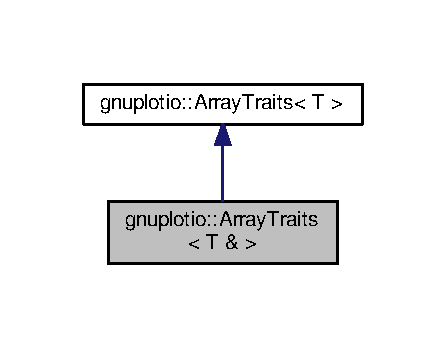
\includegraphics[width=214pt]{classgnuplotio_1_1_array_traits_3_01_t_01_6_01_4__inherit__graph}
\end{center}
\end{figure}


Collaboration diagram for gnuplotio\+:\+:Array\+Traits$<$ T \& $>$\+:\nopagebreak
\begin{figure}[H]
\begin{center}
\leavevmode
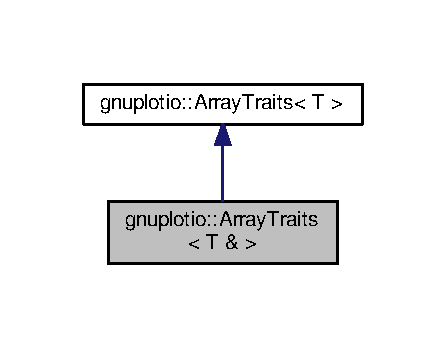
\includegraphics[width=214pt]{classgnuplotio_1_1_array_traits_3_01_t_01_6_01_4__coll__graph}
\end{center}
\end{figure}
\subsection*{Additional Inherited Members}


\subsection{Detailed Description}
\subsubsection*{template$<$typename T$>$\\*
class gnuplotio\+::\+Array\+Traits$<$ T \& $>$}



Definition at line 846 of file gnuplot-\/iostream.\+h.


\hypertarget{classgnuplotio_1_1_array_traits_3_01_t_00_01typename_01boost_1_1enable__if_3_01boost_1_1mpl_1_1a8de3a8fe198d85f7f5d28b9a2f5bf229}{}\section{gnuplotio\+:\+:Array\+Traits$<$ T, typename boost\+:\+:enable\+\_\+if$<$ boost\+:\+:mpl\+:\+:and\+\_\+$<$ is\+\_\+boost\+\_\+tuple$<$ T $>$, boost\+:\+:mpl\+:\+:not\+\_\+$<$ is\+\_\+boost\+\_\+tuple\+\_\+nulltype$<$ typename T\+:\+:tail\+\_\+type $>$ $>$ $>$ $>$\+:\+:type $>$ Class Template Reference}
\label{classgnuplotio_1_1_array_traits_3_01_t_00_01typename_01boost_1_1enable__if_3_01boost_1_1mpl_1_1a8de3a8fe198d85f7f5d28b9a2f5bf229}\index{gnuplotio\+::\+Array\+Traits$<$ T, typename boost\+::enable\+\_\+if$<$ boost\+::mpl\+::and\+\_\+$<$ is\+\_\+boost\+\_\+tuple$<$ T $>$, boost\+::mpl\+::not\+\_\+$<$ is\+\_\+boost\+\_\+tuple\+\_\+nulltype$<$ typename T\+::tail\+\_\+type $>$ $>$ $>$ $>$\+::type $>$@{gnuplotio\+::\+Array\+Traits$<$ T, typename boost\+::enable\+\_\+if$<$ boost\+::mpl\+::and\+\_\+$<$ is\+\_\+boost\+\_\+tuple$<$ T $>$, boost\+::mpl\+::not\+\_\+$<$ is\+\_\+boost\+\_\+tuple\+\_\+nulltype$<$ typename T\+::tail\+\_\+type $>$ $>$ $>$ $>$\+::type $>$}}


Inheritance diagram for gnuplotio\+:\+:Array\+Traits$<$ T, typename boost\+:\+:enable\+\_\+if$<$ boost\+:\+:mpl\+:\+:and\+\_\+$<$ is\+\_\+boost\+\_\+tuple$<$ T $>$, boost\+:\+:mpl\+:\+:not\+\_\+$<$ is\+\_\+boost\+\_\+tuple\+\_\+nulltype$<$ typename T\+:\+:tail\+\_\+type $>$ $>$ $>$ $>$\+:\+:type $>$\+:\nopagebreak
\begin{figure}[H]
\begin{center}
\leavevmode
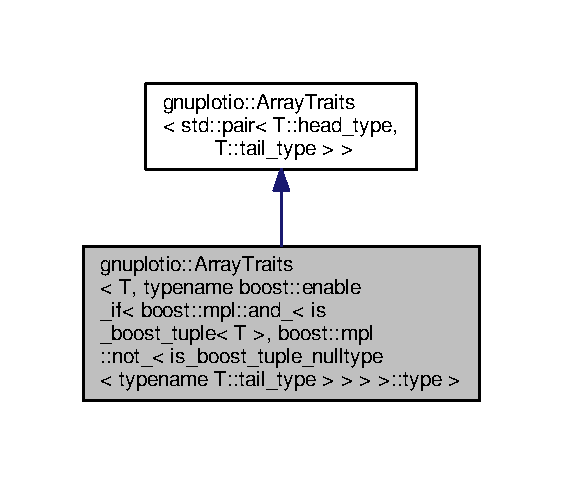
\includegraphics[width=270pt]{classgnuplotio_1_1_array_traits_3_01_t_00_01typename_01boost_1_1enable__if_3_01boost_1_1mpl_1_1a1581fe615c30084043274cbfdd41a619}
\end{center}
\end{figure}


Collaboration diagram for gnuplotio\+:\+:Array\+Traits$<$ T, typename boost\+:\+:enable\+\_\+if$<$ boost\+:\+:mpl\+:\+:and\+\_\+$<$ is\+\_\+boost\+\_\+tuple$<$ T $>$, boost\+:\+:mpl\+:\+:not\+\_\+$<$ is\+\_\+boost\+\_\+tuple\+\_\+nulltype$<$ typename T\+:\+:tail\+\_\+type $>$ $>$ $>$ $>$\+:\+:type $>$\+:\nopagebreak
\begin{figure}[H]
\begin{center}
\leavevmode
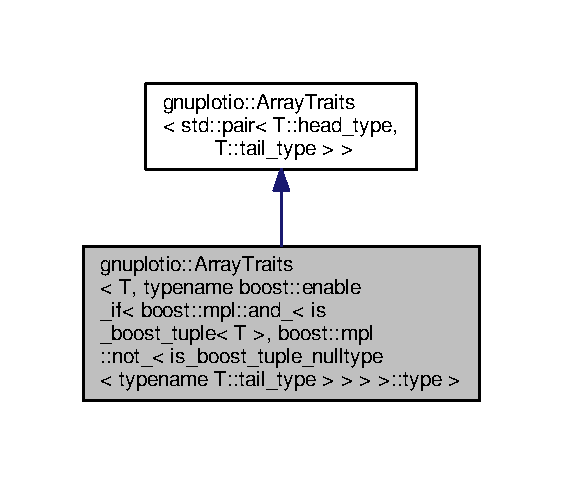
\includegraphics[width=270pt]{classgnuplotio_1_1_array_traits_3_01_t_00_01typename_01boost_1_1enable__if_3_01boost_1_1mpl_1_1aba4443da019311cdd4c31f059136bc6c}
\end{center}
\end{figure}
\subsection*{Public Types}
\begin{DoxyCompactItemize}
\item 
typedef T\+::head\+\_\+type {\bfseries HT}\hypertarget{classgnuplotio_1_1_array_traits_3_01_t_00_01typename_01boost_1_1enable__if_3_01boost_1_1mpl_1_1a8de3a8fe198d85f7f5d28b9a2f5bf229_ab56761f05b74be318cc7becbc59348df}{}\label{classgnuplotio_1_1_array_traits_3_01_t_00_01typename_01boost_1_1enable__if_3_01boost_1_1mpl_1_1a8de3a8fe198d85f7f5d28b9a2f5bf229_ab56761f05b74be318cc7becbc59348df}

\item 
typedef T\+::tail\+\_\+type {\bfseries TT}\hypertarget{classgnuplotio_1_1_array_traits_3_01_t_00_01typename_01boost_1_1enable__if_3_01boost_1_1mpl_1_1a8de3a8fe198d85f7f5d28b9a2f5bf229_a16316f598ab57b0b7ceea99dcd34632e}{}\label{classgnuplotio_1_1_array_traits_3_01_t_00_01typename_01boost_1_1enable__if_3_01boost_1_1mpl_1_1a8de3a8fe198d85f7f5d28b9a2f5bf229_a16316f598ab57b0b7ceea99dcd34632e}

\item 
typedef \hyperlink{classgnuplotio_1_1_array_traits}{Array\+Traits}$<$ typename std\+::pair$<$ HT, TT $>$ $>$ {\bfseries parent}\hypertarget{classgnuplotio_1_1_array_traits_3_01_t_00_01typename_01boost_1_1enable__if_3_01boost_1_1mpl_1_1a8de3a8fe198d85f7f5d28b9a2f5bf229_aad44f59a1d618b863442a9fdaa83d142}{}\label{classgnuplotio_1_1_array_traits_3_01_t_00_01typename_01boost_1_1enable__if_3_01boost_1_1mpl_1_1a8de3a8fe198d85f7f5d28b9a2f5bf229_aad44f59a1d618b863442a9fdaa83d142}

\end{DoxyCompactItemize}
\subsection*{Static Public Member Functions}
\begin{DoxyCompactItemize}
\item 
static \hyperlink{structgnuplotio_1_1_error___was_not_container}{parent\+::range\+\_\+type} {\bfseries get\+\_\+range} (const T \&arg)\hypertarget{classgnuplotio_1_1_array_traits_3_01_t_00_01typename_01boost_1_1enable__if_3_01boost_1_1mpl_1_1a8de3a8fe198d85f7f5d28b9a2f5bf229_aec07e01edbb46f5f283d5b6af068c0f2}{}\label{classgnuplotio_1_1_array_traits_3_01_t_00_01typename_01boost_1_1enable__if_3_01boost_1_1mpl_1_1a8de3a8fe198d85f7f5d28b9a2f5bf229_aec07e01edbb46f5f283d5b6af068c0f2}

\end{DoxyCompactItemize}
\subsection*{Additional Inherited Members}


\subsection{Detailed Description}
\subsubsection*{template$<$typename T$>$\\*
class gnuplotio\+::\+Array\+Traits$<$ T, typename boost\+::enable\+\_\+if$<$ boost\+::mpl\+::and\+\_\+$<$ is\+\_\+boost\+\_\+tuple$<$ T $>$, boost\+::mpl\+::not\+\_\+$<$ is\+\_\+boost\+\_\+tuple\+\_\+nulltype$<$ typename T\+::tail\+\_\+type $>$ $>$ $>$ $>$\+::type $>$}



Definition at line 994 of file gnuplot-\/iostream.\+h.


\hypertarget{classgnuplotio_1_1_array_traits_3_01_t_00_01typename_01boost_1_1enable__if_3_01boost_1_1mpl_1_1ad3fa8e75dccbaae12a06d17831678a88}{}\section{gnuplotio\+:\+:Array\+Traits$<$ T, typename boost\+:\+:enable\+\_\+if$<$ boost\+:\+:mpl\+:\+:and\+\_\+$<$ is\+\_\+boost\+\_\+tuple$<$ T $>$, is\+\_\+boost\+\_\+tuple\+\_\+nulltype$<$ typename T\+:\+:tail\+\_\+type $>$ $>$ $>$\+:\+:type $>$ Class Template Reference}
\label{classgnuplotio_1_1_array_traits_3_01_t_00_01typename_01boost_1_1enable__if_3_01boost_1_1mpl_1_1ad3fa8e75dccbaae12a06d17831678a88}\index{gnuplotio\+::\+Array\+Traits$<$ T, typename boost\+::enable\+\_\+if$<$ boost\+::mpl\+::and\+\_\+$<$ is\+\_\+boost\+\_\+tuple$<$ T $>$, is\+\_\+boost\+\_\+tuple\+\_\+nulltype$<$ typename T\+::tail\+\_\+type $>$ $>$ $>$\+::type $>$@{gnuplotio\+::\+Array\+Traits$<$ T, typename boost\+::enable\+\_\+if$<$ boost\+::mpl\+::and\+\_\+$<$ is\+\_\+boost\+\_\+tuple$<$ T $>$, is\+\_\+boost\+\_\+tuple\+\_\+nulltype$<$ typename T\+::tail\+\_\+type $>$ $>$ $>$\+::type $>$}}
Inheritance diagram for gnuplotio\+:\+:Array\+Traits$<$ T, typename boost\+:\+:enable\+\_\+if$<$ boost\+:\+:mpl\+:\+:and\+\_\+$<$ is\+\_\+boost\+\_\+tuple$<$ T $>$, is\+\_\+boost\+\_\+tuple\+\_\+nulltype$<$ typename T\+:\+:tail\+\_\+type $>$ $>$ $>$\+:\+:type $>$\+:\begin{figure}[H]
\begin{center}
\leavevmode
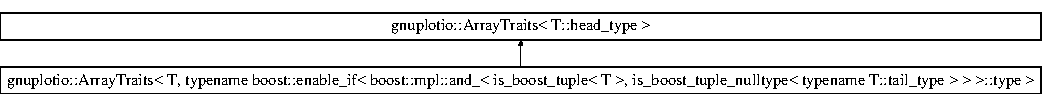
\includegraphics[height=1.259843cm]{classgnuplotio_1_1_array_traits_3_01_t_00_01typename_01boost_1_1enable__if_3_01boost_1_1mpl_1_1ad3fa8e75dccbaae12a06d17831678a88}
\end{center}
\end{figure}
\subsection*{Static Public Member Functions}
\begin{DoxyCompactItemize}
\item 
static \hyperlink{structgnuplotio_1_1_error___was_not_container}{parent\+::range\+\_\+type} {\bfseries get\+\_\+range} (const T \&arg)\hypertarget{classgnuplotio_1_1_array_traits_3_01_t_00_01typename_01boost_1_1enable__if_3_01boost_1_1mpl_1_1ad3fa8e75dccbaae12a06d17831678a88_ad0485dd16a9d54a4eb75bf3e75b1facd}{}\label{classgnuplotio_1_1_array_traits_3_01_t_00_01typename_01boost_1_1enable__if_3_01boost_1_1mpl_1_1ad3fa8e75dccbaae12a06d17831678a88_ad0485dd16a9d54a4eb75bf3e75b1facd}

\end{DoxyCompactItemize}
\subsection*{Additional Inherited Members}


\subsection{Detailed Description}
\subsubsection*{template$<$typename T$>$\\*
class gnuplotio\+::\+Array\+Traits$<$ T, typename boost\+::enable\+\_\+if$<$ boost\+::mpl\+::and\+\_\+$<$ is\+\_\+boost\+\_\+tuple$<$ T $>$, is\+\_\+boost\+\_\+tuple\+\_\+nulltype$<$ typename T\+::tail\+\_\+type $>$ $>$ $>$\+::type $>$}



Definition at line 1022 of file gnuplot-\/iostream.\+h.


\hypertarget{classgnuplotio_1_1_array_traits_3_01_t_00_01typename_01boost_1_1enable__if_3_01is__like__stl__co9e1736bbd08cd58c6993ab613a998887}{}\section{gnuplotio\+:\+:Array\+Traits$<$ T, typename boost\+:\+:enable\+\_\+if$<$ is\+\_\+like\+\_\+stl\+\_\+container$<$ T $>$ $>$\+:\+:type $>$ Class Template Reference}
\label{classgnuplotio_1_1_array_traits_3_01_t_00_01typename_01boost_1_1enable__if_3_01is__like__stl__co9e1736bbd08cd58c6993ab613a998887}\index{gnuplotio\+::\+Array\+Traits$<$ T, typename boost\+::enable\+\_\+if$<$ is\+\_\+like\+\_\+stl\+\_\+container$<$ T $>$ $>$\+::type $>$@{gnuplotio\+::\+Array\+Traits$<$ T, typename boost\+::enable\+\_\+if$<$ is\+\_\+like\+\_\+stl\+\_\+container$<$ T $>$ $>$\+::type $>$}}
Inheritance diagram for gnuplotio\+:\+:Array\+Traits$<$ T, typename boost\+:\+:enable\+\_\+if$<$ is\+\_\+like\+\_\+stl\+\_\+container$<$ T $>$ $>$\+:\+:type $>$\+:\begin{figure}[H]
\begin{center}
\leavevmode
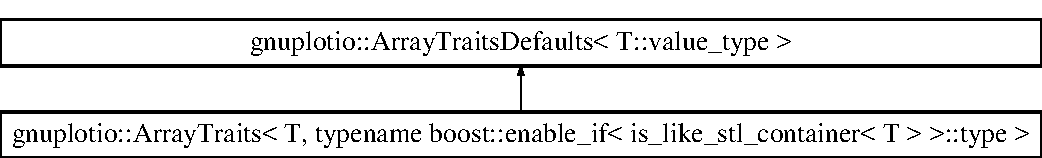
\includegraphics[height=2.000000cm]{classgnuplotio_1_1_array_traits_3_01_t_00_01typename_01boost_1_1enable__if_3_01is__like__stl__co9e1736bbd08cd58c6993ab613a998887}
\end{center}
\end{figure}
\subsection*{Public Types}
\begin{DoxyCompactItemize}
\item 
typedef \hyperlink{classgnuplotio_1_1_iterator_range}{Iterator\+Range}$<$ typename T\+::const\+\_\+iterator, typename T\+::value\+\_\+type $>$ {\bfseries range\+\_\+type}\hypertarget{classgnuplotio_1_1_array_traits_3_01_t_00_01typename_01boost_1_1enable__if_3_01is__like__stl__co9e1736bbd08cd58c6993ab613a998887_ab702072abbe018bbc90b9967ca8c4b42}{}\label{classgnuplotio_1_1_array_traits_3_01_t_00_01typename_01boost_1_1enable__if_3_01is__like__stl__co9e1736bbd08cd58c6993ab613a998887_ab702072abbe018bbc90b9967ca8c4b42}

\end{DoxyCompactItemize}
\subsection*{Static Public Member Functions}
\begin{DoxyCompactItemize}
\item 
static \hyperlink{classgnuplotio_1_1_iterator_range}{range\+\_\+type} {\bfseries get\+\_\+range} (const T \&arg)\hypertarget{classgnuplotio_1_1_array_traits_3_01_t_00_01typename_01boost_1_1enable__if_3_01is__like__stl__co9e1736bbd08cd58c6993ab613a998887_a89d4150ab3c479cde972071a10acd27b}{}\label{classgnuplotio_1_1_array_traits_3_01_t_00_01typename_01boost_1_1enable__if_3_01is__like__stl__co9e1736bbd08cd58c6993ab613a998887_a89d4150ab3c479cde972071a10acd27b}

\end{DoxyCompactItemize}
\subsection*{Additional Inherited Members}


\subsection{Detailed Description}
\subsubsection*{template$<$typename T$>$\\*
class gnuplotio\+::\+Array\+Traits$<$ T, typename boost\+::enable\+\_\+if$<$ is\+\_\+like\+\_\+stl\+\_\+container$<$ T $>$ $>$\+::type $>$}



Definition at line 897 of file gnuplot-\/iostream.\+h.


\hypertarget{classgnuplotio_1_1_array_traits_3_01_t[_n]_4}{}\section{gnuplotio\+:\+:Array\+Traits$<$ T\mbox{[}N\mbox{]}$>$ Class Template Reference}
\label{classgnuplotio_1_1_array_traits_3_01_t[_n]_4}\index{gnuplotio\+::\+Array\+Traits$<$ T\mbox{[}\+N\mbox{]}$>$@{gnuplotio\+::\+Array\+Traits$<$ T[N]$>$}}


Inheritance diagram for gnuplotio\+:\+:Array\+Traits$<$ T\mbox{[}N\mbox{]}$>$\+:\nopagebreak
\begin{figure}[H]
\begin{center}
\leavevmode
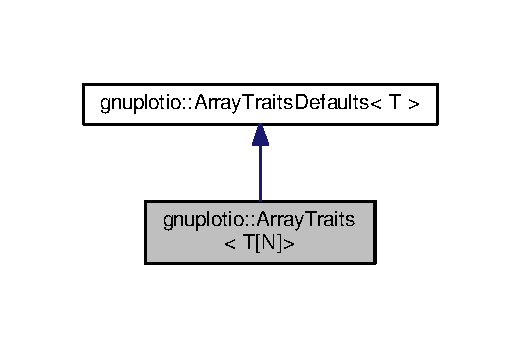
\includegraphics[width=250pt]{classgnuplotio_1_1_array_traits_3_01_t[_n]_4__inherit__graph}
\end{center}
\end{figure}


Collaboration diagram for gnuplotio\+:\+:Array\+Traits$<$ T\mbox{[}N\mbox{]}$>$\+:\nopagebreak
\begin{figure}[H]
\begin{center}
\leavevmode
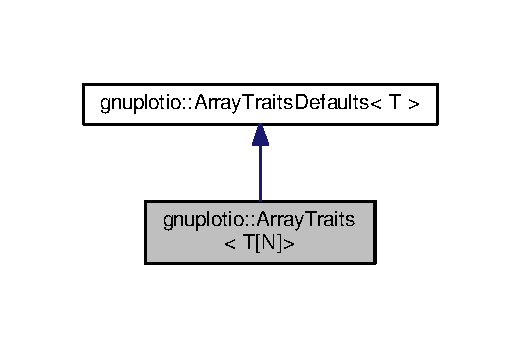
\includegraphics[width=250pt]{classgnuplotio_1_1_array_traits_3_01_t[_n]_4__coll__graph}
\end{center}
\end{figure}
\subsection*{Public Types}
\begin{DoxyCompactItemize}
\item 
typedef \hyperlink{classgnuplotio_1_1_iterator_range}{Iterator\+Range}$<$ const T $\ast$, T $>$ {\bfseries range\+\_\+type}\hypertarget{classgnuplotio_1_1_array_traits_3_01_t[_n]_4_a926f3c3d14fbe82aab7b70ccc16d20fb}{}\label{classgnuplotio_1_1_array_traits_3_01_t[_n]_4_a926f3c3d14fbe82aab7b70ccc16d20fb}

\end{DoxyCompactItemize}
\subsection*{Static Public Member Functions}
\begin{DoxyCompactItemize}
\item 
static \hyperlink{classgnuplotio_1_1_iterator_range}{range\+\_\+type} {\bfseries get\+\_\+range} (const T(\&arg)\mbox{[}N\mbox{]})\hypertarget{classgnuplotio_1_1_array_traits_3_01_t[_n]_4_adc9c1ce6da4923418f367e08c150a928}{}\label{classgnuplotio_1_1_array_traits_3_01_t[_n]_4_adc9c1ce6da4923418f367e08c150a928}

\end{DoxyCompactItemize}
\subsection*{Additional Inherited Members}


\subsection{Detailed Description}
\subsubsection*{template$<$typename T, size\+\_\+t N$>$\\*
class gnuplotio\+::\+Array\+Traits$<$ T\mbox{[}\+N\mbox{]}$>$}



Definition at line 913 of file gnuplot-\/iostream.\+h.


\hypertarget{classgnuplotio_1_1_array_traits_defaults}{}\section{gnuplotio\+:\+:Array\+Traits\+Defaults$<$ V $>$ Class Template Reference}
\label{classgnuplotio_1_1_array_traits_defaults}\index{gnuplotio\+::\+Array\+Traits\+Defaults$<$ V $>$@{gnuplotio\+::\+Array\+Traits\+Defaults$<$ V $>$}}
\subsection*{Public Types}
\begin{DoxyCompactItemize}
\item 
typedef V {\bfseries value\+\_\+type}\hypertarget{classgnuplotio_1_1_array_traits_defaults_ad7a9e8d19419fabe2ab9cc1b76c9965b}{}\label{classgnuplotio_1_1_array_traits_defaults_ad7a9e8d19419fabe2ab9cc1b76c9965b}

\end{DoxyCompactItemize}
\subsection*{Static Public Attributes}
\begin{DoxyCompactItemize}
\item 
static const bool {\bfseries is\+\_\+container} = true\hypertarget{classgnuplotio_1_1_array_traits_defaults_a57bab5bf3617f0ee66fdd4dcb751aa21}{}\label{classgnuplotio_1_1_array_traits_defaults_a57bab5bf3617f0ee66fdd4dcb751aa21}

\item 
static const bool {\bfseries allow\+\_\+auto\+\_\+unwrap} = true\hypertarget{classgnuplotio_1_1_array_traits_defaults_ac8d430cba6ceefc6f52706455f12a0e8}{}\label{classgnuplotio_1_1_array_traits_defaults_ac8d430cba6ceefc6f52706455f12a0e8}

\item 
static const size\+\_\+t {\bfseries depth} = \hyperlink{classgnuplotio_1_1_array_traits}{Array\+Traits}$<$V$>$\+::depth + 1\hypertarget{classgnuplotio_1_1_array_traits_defaults_ac51367f5da9096249b162af1496e36ab}{}\label{classgnuplotio_1_1_array_traits_defaults_ac51367f5da9096249b162af1496e36ab}

\end{DoxyCompactItemize}


\subsection{Detailed Description}
\subsubsection*{template$<$typename V$>$\\*
class gnuplotio\+::\+Array\+Traits\+Defaults$<$ V $>$}



Definition at line 833 of file gnuplot-\/iostream.\+h.


\hypertarget{structgnuplotio_1_1_binary_sender}{}\section{gnuplotio\+:\+:Binary\+Sender$<$ T, Enable $>$ Struct Template Reference}
\label{structgnuplotio_1_1_binary_sender}\index{gnuplotio\+::\+Binary\+Sender$<$ T, Enable $>$@{gnuplotio\+::\+Binary\+Sender$<$ T, Enable $>$}}
\subsection*{Public Member Functions}
\begin{DoxyCompactItemize}
\item 
{\bfseries G\+N\+U\+P\+L\+O\+T\+\_\+\+S\+T\+A\+T\+I\+C\+\_\+\+A\+S\+S\+E\+R\+T\+\_\+\+M\+SG} ((sizeof(T)==0),\char`\"{}Binary\+Sender class not specialized for this type\char`\"{})\hypertarget{structgnuplotio_1_1_binary_sender_a165c59a28adc4a90930925c6e0bfb0a9}{}\label{structgnuplotio_1_1_binary_sender_a165c59a28adc4a90930925c6e0bfb0a9}

\end{DoxyCompactItemize}
\subsection*{Static Public Member Functions}
\begin{DoxyCompactItemize}
\item 
static void {\bfseries send} (std\+::ostream \&stream, const T \&v)\hypertarget{structgnuplotio_1_1_binary_sender_a4b5dd22b7679c4f0ce4d8e75b36c8a21}{}\label{structgnuplotio_1_1_binary_sender_a4b5dd22b7679c4f0ce4d8e75b36c8a21}

\end{DoxyCompactItemize}


\subsection{Detailed Description}
\subsubsection*{template$<$typename T, typename Enable = void$>$\\*
struct gnuplotio\+::\+Binary\+Sender$<$ T, Enable $>$}



Definition at line 441 of file gnuplot-\/iostream.\+h.


\hypertarget{structgnuplotio_1_1_binary_sender_3_01boost_1_1int16__t_01_4}{}\section{gnuplotio\+:\+:Binary\+Sender$<$ boost\+:\+:int16\+\_\+t $>$ Struct Template Reference}
\label{structgnuplotio_1_1_binary_sender_3_01boost_1_1int16__t_01_4}\index{gnuplotio\+::\+Binary\+Sender$<$ boost\+::int16\+\_\+t $>$@{gnuplotio\+::\+Binary\+Sender$<$ boost\+::int16\+\_\+t $>$}}


Inheritance diagram for gnuplotio\+:\+:Binary\+Sender$<$ boost\+:\+:int16\+\_\+t $>$\+:\nopagebreak
\begin{figure}[H]
\begin{center}
\leavevmode
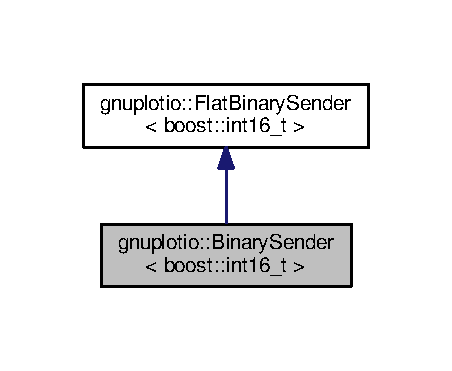
\includegraphics[width=217pt]{structgnuplotio_1_1_binary_sender_3_01boost_1_1int16__t_01_4__inherit__graph}
\end{center}
\end{figure}


Collaboration diagram for gnuplotio\+:\+:Binary\+Sender$<$ boost\+:\+:int16\+\_\+t $>$\+:\nopagebreak
\begin{figure}[H]
\begin{center}
\leavevmode
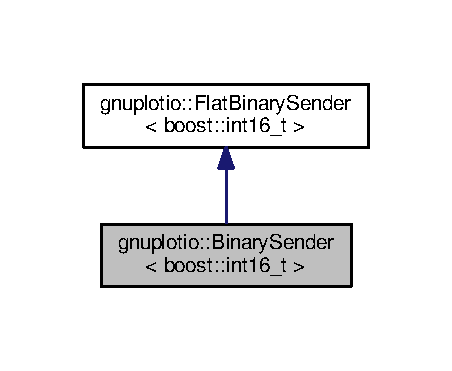
\includegraphics[width=217pt]{structgnuplotio_1_1_binary_sender_3_01boost_1_1int16__t_01_4__coll__graph}
\end{center}
\end{figure}
\subsection*{Additional Inherited Members}


\subsection{Detailed Description}
\subsubsection*{template$<$$>$\\*
struct gnuplotio\+::\+Binary\+Sender$<$ boost\+::int16\+\_\+t $>$}



Definition at line 485 of file gnuplot-\/iostream.\+h.


\hypertarget{structgnuplotio_1_1_binary_sender_3_01boost_1_1int32__t_01_4}{}\section{gnuplotio\+:\+:Binary\+Sender$<$ boost\+:\+:int32\+\_\+t $>$ Struct Template Reference}
\label{structgnuplotio_1_1_binary_sender_3_01boost_1_1int32__t_01_4}\index{gnuplotio\+::\+Binary\+Sender$<$ boost\+::int32\+\_\+t $>$@{gnuplotio\+::\+Binary\+Sender$<$ boost\+::int32\+\_\+t $>$}}


Inheritance diagram for gnuplotio\+:\+:Binary\+Sender$<$ boost\+:\+:int32\+\_\+t $>$\+:\nopagebreak
\begin{figure}[H]
\begin{center}
\leavevmode
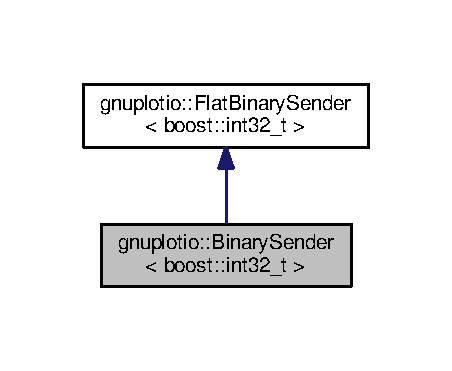
\includegraphics[width=217pt]{structgnuplotio_1_1_binary_sender_3_01boost_1_1int32__t_01_4__inherit__graph}
\end{center}
\end{figure}


Collaboration diagram for gnuplotio\+:\+:Binary\+Sender$<$ boost\+:\+:int32\+\_\+t $>$\+:\nopagebreak
\begin{figure}[H]
\begin{center}
\leavevmode
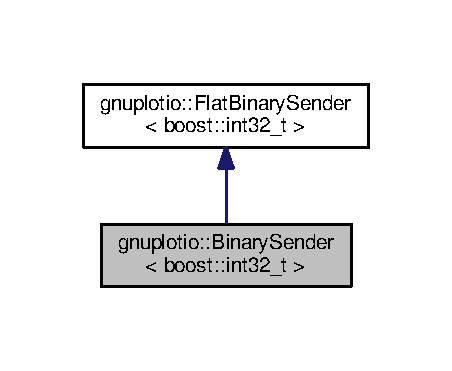
\includegraphics[width=217pt]{structgnuplotio_1_1_binary_sender_3_01boost_1_1int32__t_01_4__coll__graph}
\end{center}
\end{figure}
\subsection*{Additional Inherited Members}


\subsection{Detailed Description}
\subsubsection*{template$<$$>$\\*
struct gnuplotio\+::\+Binary\+Sender$<$ boost\+::int32\+\_\+t $>$}



Definition at line 487 of file gnuplot-\/iostream.\+h.


\hypertarget{structgnuplotio_1_1_binary_sender_3_01boost_1_1int64__t_01_4}{}\section{gnuplotio\+:\+:Binary\+Sender$<$ boost\+:\+:int64\+\_\+t $>$ Struct Template Reference}
\label{structgnuplotio_1_1_binary_sender_3_01boost_1_1int64__t_01_4}\index{gnuplotio\+::\+Binary\+Sender$<$ boost\+::int64\+\_\+t $>$@{gnuplotio\+::\+Binary\+Sender$<$ boost\+::int64\+\_\+t $>$}}


Inheritance diagram for gnuplotio\+:\+:Binary\+Sender$<$ boost\+:\+:int64\+\_\+t $>$\+:\nopagebreak
\begin{figure}[H]
\begin{center}
\leavevmode
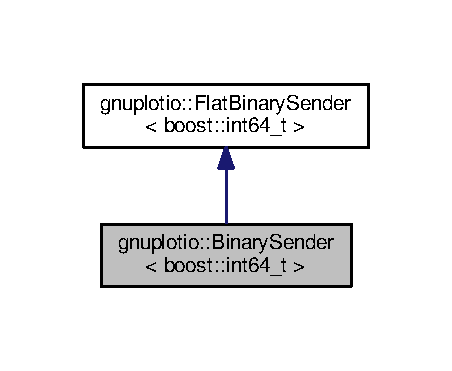
\includegraphics[width=217pt]{structgnuplotio_1_1_binary_sender_3_01boost_1_1int64__t_01_4__inherit__graph}
\end{center}
\end{figure}


Collaboration diagram for gnuplotio\+:\+:Binary\+Sender$<$ boost\+:\+:int64\+\_\+t $>$\+:\nopagebreak
\begin{figure}[H]
\begin{center}
\leavevmode
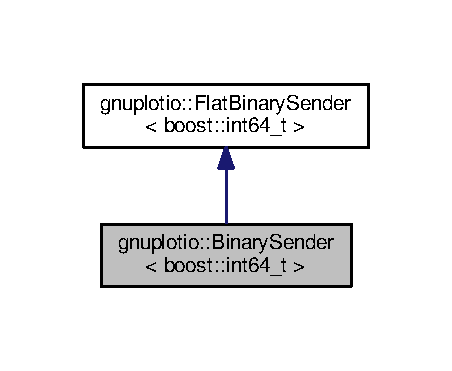
\includegraphics[width=217pt]{structgnuplotio_1_1_binary_sender_3_01boost_1_1int64__t_01_4__coll__graph}
\end{center}
\end{figure}
\subsection*{Additional Inherited Members}


\subsection{Detailed Description}
\subsubsection*{template$<$$>$\\*
struct gnuplotio\+::\+Binary\+Sender$<$ boost\+::int64\+\_\+t $>$}



Definition at line 489 of file gnuplot-\/iostream.\+h.


\hypertarget{structgnuplotio_1_1_binary_sender_3_01boost_1_1int8__t_01_4}{}\section{gnuplotio\+:\+:Binary\+Sender$<$ boost\+:\+:int8\+\_\+t $>$ Struct Template Reference}
\label{structgnuplotio_1_1_binary_sender_3_01boost_1_1int8__t_01_4}\index{gnuplotio\+::\+Binary\+Sender$<$ boost\+::int8\+\_\+t $>$@{gnuplotio\+::\+Binary\+Sender$<$ boost\+::int8\+\_\+t $>$}}
Inheritance diagram for gnuplotio\+:\+:Binary\+Sender$<$ boost\+:\+:int8\+\_\+t $>$\+:\begin{figure}[H]
\begin{center}
\leavevmode
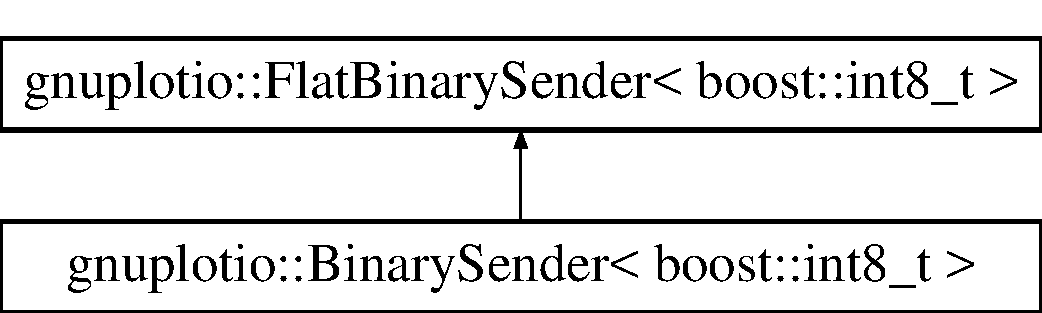
\includegraphics[height=2.000000cm]{structgnuplotio_1_1_binary_sender_3_01boost_1_1int8__t_01_4}
\end{center}
\end{figure}
\subsection*{Additional Inherited Members}


\subsection{Detailed Description}
\subsubsection*{template$<$$>$\\*
struct gnuplotio\+::\+Binary\+Sender$<$ boost\+::int8\+\_\+t $>$}



Definition at line 483 of file gnuplot-\/iostream.\+h.


\hypertarget{structgnuplotio_1_1_binary_sender_3_01boost_1_1uint16__t_01_4}{}\section{gnuplotio\+:\+:Binary\+Sender$<$ boost\+:\+:uint16\+\_\+t $>$ Struct Template Reference}
\label{structgnuplotio_1_1_binary_sender_3_01boost_1_1uint16__t_01_4}\index{gnuplotio\+::\+Binary\+Sender$<$ boost\+::uint16\+\_\+t $>$@{gnuplotio\+::\+Binary\+Sender$<$ boost\+::uint16\+\_\+t $>$}}


Inheritance diagram for gnuplotio\+:\+:Binary\+Sender$<$ boost\+:\+:uint16\+\_\+t $>$\+:\nopagebreak
\begin{figure}[H]
\begin{center}
\leavevmode
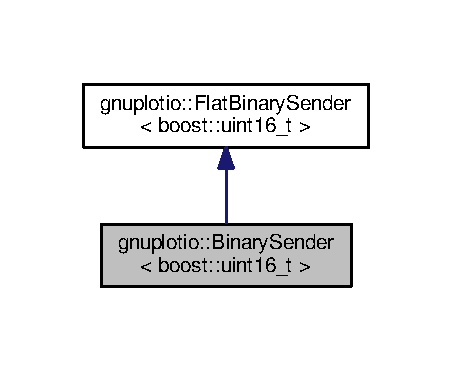
\includegraphics[width=217pt]{structgnuplotio_1_1_binary_sender_3_01boost_1_1uint16__t_01_4__inherit__graph}
\end{center}
\end{figure}


Collaboration diagram for gnuplotio\+:\+:Binary\+Sender$<$ boost\+:\+:uint16\+\_\+t $>$\+:\nopagebreak
\begin{figure}[H]
\begin{center}
\leavevmode
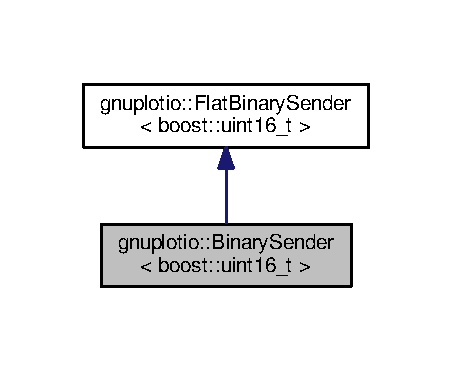
\includegraphics[width=217pt]{structgnuplotio_1_1_binary_sender_3_01boost_1_1uint16__t_01_4__coll__graph}
\end{center}
\end{figure}
\subsection*{Additional Inherited Members}


\subsection{Detailed Description}
\subsubsection*{template$<$$>$\\*
struct gnuplotio\+::\+Binary\+Sender$<$ boost\+::uint16\+\_\+t $>$}



Definition at line 486 of file gnuplot-\/iostream.\+h.


\hypertarget{structgnuplotio_1_1_binary_sender_3_01boost_1_1uint32__t_01_4}{}\section{gnuplotio\+:\+:Binary\+Sender$<$ boost\+:\+:uint32\+\_\+t $>$ Struct Template Reference}
\label{structgnuplotio_1_1_binary_sender_3_01boost_1_1uint32__t_01_4}\index{gnuplotio\+::\+Binary\+Sender$<$ boost\+::uint32\+\_\+t $>$@{gnuplotio\+::\+Binary\+Sender$<$ boost\+::uint32\+\_\+t $>$}}


Inheritance diagram for gnuplotio\+:\+:Binary\+Sender$<$ boost\+:\+:uint32\+\_\+t $>$\+:
\nopagebreak
\begin{figure}[H]
\begin{center}
\leavevmode
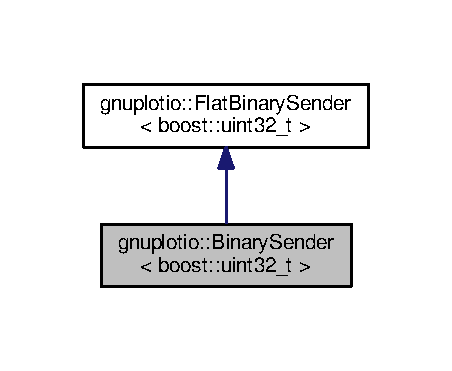
\includegraphics[width=217pt]{structgnuplotio_1_1_binary_sender_3_01boost_1_1uint32__t_01_4__inherit__graph}
\end{center}
\end{figure}


Collaboration diagram for gnuplotio\+:\+:Binary\+Sender$<$ boost\+:\+:uint32\+\_\+t $>$\+:
\nopagebreak
\begin{figure}[H]
\begin{center}
\leavevmode
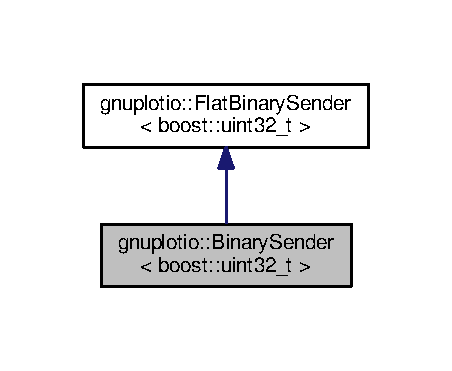
\includegraphics[width=217pt]{structgnuplotio_1_1_binary_sender_3_01boost_1_1uint32__t_01_4__coll__graph}
\end{center}
\end{figure}
\subsection*{Additional Inherited Members}


\subsection{Detailed Description}
\subsubsection*{template$<$$>$\\*
struct gnuplotio\+::\+Binary\+Sender$<$ boost\+::uint32\+\_\+t $>$}



Definition at line 488 of file gnuplot-\/iostream.\+h.


\hypertarget{structgnuplotio_1_1_binary_sender_3_01boost_1_1uint64__t_01_4}{}\section{gnuplotio\+:\+:Binary\+Sender$<$ boost\+:\+:uint64\+\_\+t $>$ Struct Template Reference}
\label{structgnuplotio_1_1_binary_sender_3_01boost_1_1uint64__t_01_4}\index{gnuplotio\+::\+Binary\+Sender$<$ boost\+::uint64\+\_\+t $>$@{gnuplotio\+::\+Binary\+Sender$<$ boost\+::uint64\+\_\+t $>$}}
Inheritance diagram for gnuplotio\+:\+:Binary\+Sender$<$ boost\+:\+:uint64\+\_\+t $>$\+:\begin{figure}[H]
\begin{center}
\leavevmode
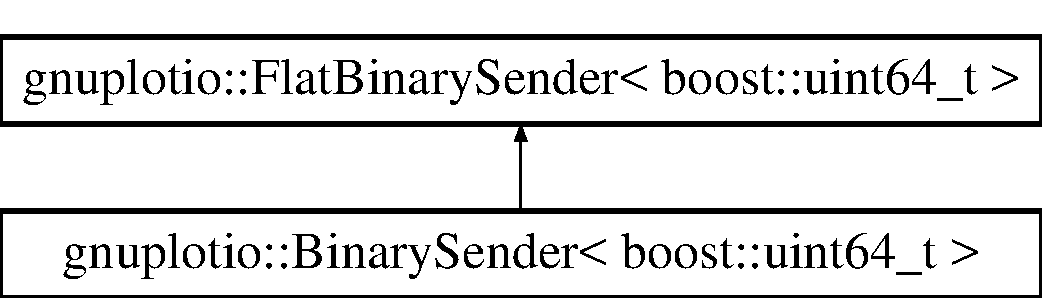
\includegraphics[height=2.000000cm]{structgnuplotio_1_1_binary_sender_3_01boost_1_1uint64__t_01_4}
\end{center}
\end{figure}
\subsection*{Additional Inherited Members}


\subsection{Detailed Description}
\subsubsection*{template$<$$>$\\*
struct gnuplotio\+::\+Binary\+Sender$<$ boost\+::uint64\+\_\+t $>$}



Definition at line 490 of file gnuplot-\/iostream.\+h.


\hypertarget{structgnuplotio_1_1_binary_sender_3_01boost_1_1uint8__t_01_4}{}\section{gnuplotio\+:\+:Binary\+Sender$<$ boost\+:\+:uint8\+\_\+t $>$ Struct Template Reference}
\label{structgnuplotio_1_1_binary_sender_3_01boost_1_1uint8__t_01_4}\index{gnuplotio\+::\+Binary\+Sender$<$ boost\+::uint8\+\_\+t $>$@{gnuplotio\+::\+Binary\+Sender$<$ boost\+::uint8\+\_\+t $>$}}


Inheritance diagram for gnuplotio\+:\+:Binary\+Sender$<$ boost\+:\+:uint8\+\_\+t $>$\+:
\nopagebreak
\begin{figure}[H]
\begin{center}
\leavevmode
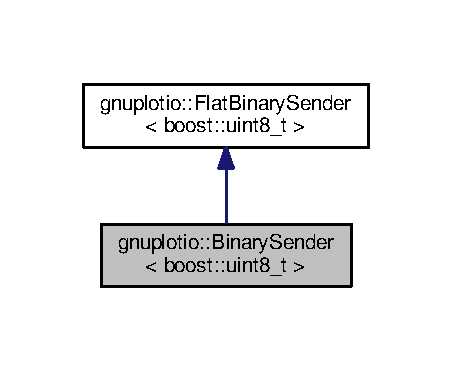
\includegraphics[width=217pt]{structgnuplotio_1_1_binary_sender_3_01boost_1_1uint8__t_01_4__inherit__graph}
\end{center}
\end{figure}


Collaboration diagram for gnuplotio\+:\+:Binary\+Sender$<$ boost\+:\+:uint8\+\_\+t $>$\+:
\nopagebreak
\begin{figure}[H]
\begin{center}
\leavevmode
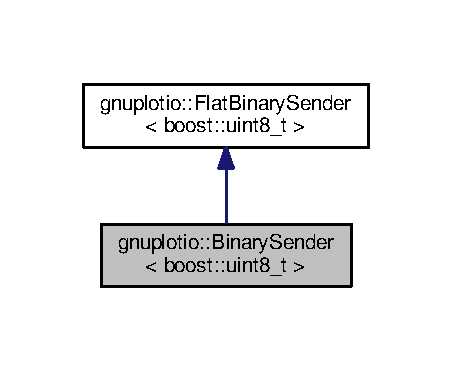
\includegraphics[width=217pt]{structgnuplotio_1_1_binary_sender_3_01boost_1_1uint8__t_01_4__coll__graph}
\end{center}
\end{figure}
\subsection*{Additional Inherited Members}


\subsection{Detailed Description}
\subsubsection*{template$<$$>$\\*
struct gnuplotio\+::\+Binary\+Sender$<$ boost\+::uint8\+\_\+t $>$}



Definition at line 484 of file gnuplot-\/iostream.\+h.


\hypertarget{structgnuplotio_1_1_binary_sender_3_01double_01_4}{}\section{gnuplotio\+:\+:Binary\+Sender$<$ double $>$ Struct Template Reference}
\label{structgnuplotio_1_1_binary_sender_3_01double_01_4}\index{gnuplotio\+::\+Binary\+Sender$<$ double $>$@{gnuplotio\+::\+Binary\+Sender$<$ double $>$}}
Inheritance diagram for gnuplotio\+:\+:Binary\+Sender$<$ double $>$\+:\begin{figure}[H]
\begin{center}
\leavevmode
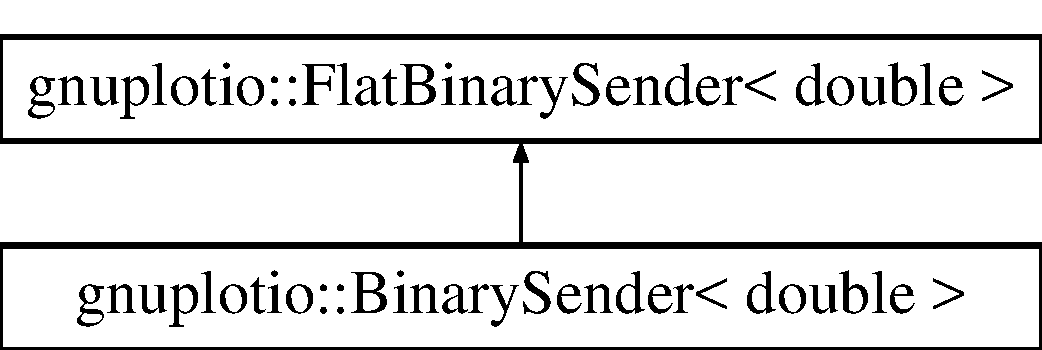
\includegraphics[height=2.000000cm]{structgnuplotio_1_1_binary_sender_3_01double_01_4}
\end{center}
\end{figure}
\subsection*{Additional Inherited Members}


\subsection{Detailed Description}
\subsubsection*{template$<$$>$\\*
struct gnuplotio\+::\+Binary\+Sender$<$ double $>$}



Definition at line 482 of file gnuplot-\/iostream.\+h.


\hypertarget{structgnuplotio_1_1_binary_sender_3_01float_01_4}{}\section{gnuplotio\+:\+:Binary\+Sender$<$ float $>$ Struct Template Reference}
\label{structgnuplotio_1_1_binary_sender_3_01float_01_4}\index{gnuplotio\+::\+Binary\+Sender$<$ float $>$@{gnuplotio\+::\+Binary\+Sender$<$ float $>$}}


Inheritance diagram for gnuplotio\+:\+:Binary\+Sender$<$ float $>$\+:
\nopagebreak
\begin{figure}[H]
\begin{center}
\leavevmode
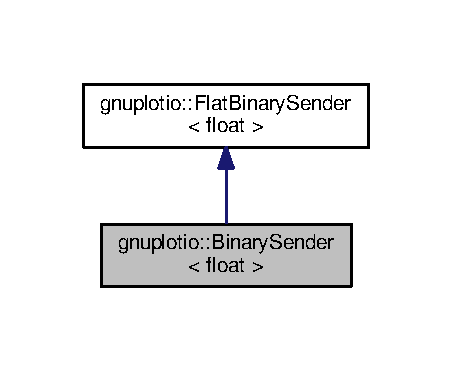
\includegraphics[width=217pt]{structgnuplotio_1_1_binary_sender_3_01float_01_4__inherit__graph}
\end{center}
\end{figure}


Collaboration diagram for gnuplotio\+:\+:Binary\+Sender$<$ float $>$\+:
\nopagebreak
\begin{figure}[H]
\begin{center}
\leavevmode
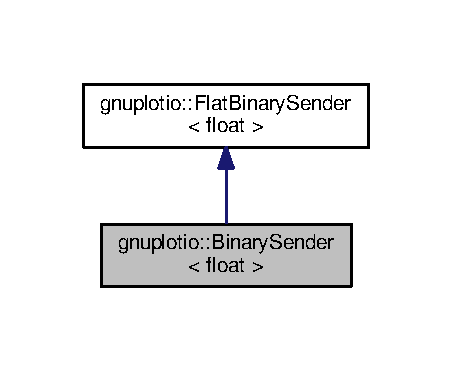
\includegraphics[width=217pt]{structgnuplotio_1_1_binary_sender_3_01float_01_4__coll__graph}
\end{center}
\end{figure}
\subsection*{Additional Inherited Members}


\subsection{Detailed Description}
\subsubsection*{template$<$$>$\\*
struct gnuplotio\+::\+Binary\+Sender$<$ float $>$}



Definition at line 481 of file gnuplot-\/iostream.\+h.


\hypertarget{structgnuplotio_1_1_binary_sender_3_01std_1_1complex_3_01_t_01_4_01_4}{}\section{gnuplotio\+:\+:Binary\+Sender$<$ std\+:\+:complex$<$ T $>$ $>$ Struct Template Reference}
\label{structgnuplotio_1_1_binary_sender_3_01std_1_1complex_3_01_t_01_4_01_4}\index{gnuplotio\+::\+Binary\+Sender$<$ std\+::complex$<$ T $>$ $>$@{gnuplotio\+::\+Binary\+Sender$<$ std\+::complex$<$ T $>$ $>$}}
\subsection*{Static Public Member Functions}
\begin{DoxyCompactItemize}
\item 
static void {\bfseries send} (std\+::ostream \&stream, const std\+::complex$<$ T $>$ \&v)\hypertarget{structgnuplotio_1_1_binary_sender_3_01std_1_1complex_3_01_t_01_4_01_4_a759de700a1cd68000830a4b15a6fec49}{}\label{structgnuplotio_1_1_binary_sender_3_01std_1_1complex_3_01_t_01_4_01_4_a759de700a1cd68000830a4b15a6fec49}

\end{DoxyCompactItemize}


\subsection{Detailed Description}
\subsubsection*{template$<$typename T$>$\\*
struct gnuplotio\+::\+Binary\+Sender$<$ std\+::complex$<$ T $>$ $>$}



Definition at line 565 of file gnuplot-\/iostream.\+h.


\hypertarget{structgnuplotio_1_1_binary_sender_3_01std_1_1pair_3_01_t_00_01_u_01_4_01_4}{}\section{gnuplotio\+:\+:Binary\+Sender$<$ std\+:\+:pair$<$ T, U $>$ $>$ Struct Template Reference}
\label{structgnuplotio_1_1_binary_sender_3_01std_1_1pair_3_01_t_00_01_u_01_4_01_4}\index{gnuplotio\+::\+Binary\+Sender$<$ std\+::pair$<$ T, U $>$ $>$@{gnuplotio\+::\+Binary\+Sender$<$ std\+::pair$<$ T, U $>$ $>$}}
\subsection*{Static Public Member Functions}
\begin{DoxyCompactItemize}
\item 
static void {\bfseries send} (std\+::ostream \&stream, const std\+::pair$<$ T, U $>$ \&v)\hypertarget{structgnuplotio_1_1_binary_sender_3_01std_1_1pair_3_01_t_00_01_u_01_4_01_4_a9d949c8e7b1dea493288b0a2dd95cbff}{}\label{structgnuplotio_1_1_binary_sender_3_01std_1_1pair_3_01_t_00_01_u_01_4_01_4_a9d949c8e7b1dea493288b0a2dd95cbff}

\end{DoxyCompactItemize}


\subsection{Detailed Description}
\subsubsection*{template$<$typename T, typename U$>$\\*
struct gnuplotio\+::\+Binary\+Sender$<$ std\+::pair$<$ T, U $>$ $>$}



Definition at line 536 of file gnuplot-\/iostream.\+h.


\hypertarget{structgnuplotio_1_1_binary_sender_3_01_t_00_01typename_01boost_1_1enable__if_3_01boost_1_1mpl_1_916ff7a758aa0b8917fd3b30ff275f06}{}\section{gnuplotio\+:\+:Binary\+Sender$<$ T, typename boost\+:\+:enable\+\_\+if$<$ boost\+:\+:mpl\+:\+:and\+\_\+$<$ is\+\_\+boost\+\_\+tuple$<$ T $>$, boost\+:\+:mpl\+:\+:not\+\_\+$<$ is\+\_\+boost\+\_\+tuple\+\_\+nulltype$<$ typename T\+:\+:tail\+\_\+type $>$ $>$ $>$ $>$\+:\+:type $>$ Struct Template Reference}
\label{structgnuplotio_1_1_binary_sender_3_01_t_00_01typename_01boost_1_1enable__if_3_01boost_1_1mpl_1_916ff7a758aa0b8917fd3b30ff275f06}\index{gnuplotio\+::\+Binary\+Sender$<$ T, typename boost\+::enable\+\_\+if$<$ boost\+::mpl\+::and\+\_\+$<$ is\+\_\+boost\+\_\+tuple$<$ T $>$, boost\+::mpl\+::not\+\_\+$<$ is\+\_\+boost\+\_\+tuple\+\_\+nulltype$<$ typename T\+::tail\+\_\+type $>$ $>$ $>$ $>$\+::type $>$@{gnuplotio\+::\+Binary\+Sender$<$ T, typename boost\+::enable\+\_\+if$<$ boost\+::mpl\+::and\+\_\+$<$ is\+\_\+boost\+\_\+tuple$<$ T $>$, boost\+::mpl\+::not\+\_\+$<$ is\+\_\+boost\+\_\+tuple\+\_\+nulltype$<$ typename T\+::tail\+\_\+type $>$ $>$ $>$ $>$\+::type $>$}}
\subsection*{Static Public Member Functions}
\begin{DoxyCompactItemize}
\item 
static void {\bfseries send} (std\+::ostream \&stream, const T \&v)\hypertarget{structgnuplotio_1_1_binary_sender_3_01_t_00_01typename_01boost_1_1enable__if_3_01boost_1_1mpl_1_916ff7a758aa0b8917fd3b30ff275f06_a90bdbe9d299646a871882da19fdb30a9}{}\label{structgnuplotio_1_1_binary_sender_3_01_t_00_01typename_01boost_1_1enable__if_3_01boost_1_1mpl_1_916ff7a758aa0b8917fd3b30ff275f06_a90bdbe9d299646a871882da19fdb30a9}

\end{DoxyCompactItemize}


\subsection{Detailed Description}
\subsubsection*{template$<$typename T$>$\\*
struct gnuplotio\+::\+Binary\+Sender$<$ T, typename boost\+::enable\+\_\+if$<$ boost\+::mpl\+::and\+\_\+$<$ is\+\_\+boost\+\_\+tuple$<$ T $>$, boost\+::mpl\+::not\+\_\+$<$ is\+\_\+boost\+\_\+tuple\+\_\+nulltype$<$ typename T\+::tail\+\_\+type $>$ $>$ $>$ $>$\+::type $>$}



Definition at line 637 of file gnuplot-\/iostream.\+h.


\hypertarget{structgnuplotio_1_1_binary_sender_3_01_t_00_01typename_01boost_1_1enable__if_3_01boost_1_1mpl_1_29e1098ca8b7afc20f2ca0bc2e79506a}{}\section{gnuplotio\+:\+:Binary\+Sender$<$ T, typename boost\+:\+:enable\+\_\+if$<$ boost\+:\+:mpl\+:\+:and\+\_\+$<$ is\+\_\+boost\+\_\+tuple$<$ T $>$, is\+\_\+boost\+\_\+tuple\+\_\+nulltype$<$ typename T\+:\+:tail\+\_\+type $>$ $>$ $>$\+:\+:type $>$ Struct Template Reference}
\label{structgnuplotio_1_1_binary_sender_3_01_t_00_01typename_01boost_1_1enable__if_3_01boost_1_1mpl_1_29e1098ca8b7afc20f2ca0bc2e79506a}\index{gnuplotio\+::\+Binary\+Sender$<$ T, typename boost\+::enable\+\_\+if$<$ boost\+::mpl\+::and\+\_\+$<$ is\+\_\+boost\+\_\+tuple$<$ T $>$, is\+\_\+boost\+\_\+tuple\+\_\+nulltype$<$ typename T\+::tail\+\_\+type $>$ $>$ $>$\+::type $>$@{gnuplotio\+::\+Binary\+Sender$<$ T, typename boost\+::enable\+\_\+if$<$ boost\+::mpl\+::and\+\_\+$<$ is\+\_\+boost\+\_\+tuple$<$ T $>$, is\+\_\+boost\+\_\+tuple\+\_\+nulltype$<$ typename T\+::tail\+\_\+type $>$ $>$ $>$\+::type $>$}}
\subsection*{Static Public Member Functions}
\begin{DoxyCompactItemize}
\item 
static void {\bfseries send} (std\+::ostream \&stream, const T \&v)\hypertarget{structgnuplotio_1_1_binary_sender_3_01_t_00_01typename_01boost_1_1enable__if_3_01boost_1_1mpl_1_29e1098ca8b7afc20f2ca0bc2e79506a_a50e54b7f2aba37f1f9e63fa81941b6d6}{}\label{structgnuplotio_1_1_binary_sender_3_01_t_00_01typename_01boost_1_1enable__if_3_01boost_1_1mpl_1_29e1098ca8b7afc20f2ca0bc2e79506a_a50e54b7f2aba37f1f9e63fa81941b6d6}

\end{DoxyCompactItemize}


\subsection{Detailed Description}
\subsubsection*{template$<$typename T$>$\\*
struct gnuplotio\+::\+Binary\+Sender$<$ T, typename boost\+::enable\+\_\+if$<$ boost\+::mpl\+::and\+\_\+$<$ is\+\_\+boost\+\_\+tuple$<$ T $>$, is\+\_\+boost\+\_\+tuple\+\_\+nulltype$<$ typename T\+::tail\+\_\+type $>$ $>$ $>$\+::type $>$}



Definition at line 652 of file gnuplot-\/iostream.\+h.


\hypertarget{structgnuplotio_1_1_binfmt_sender}{}\section{gnuplotio\+:\+:Binfmt\+Sender$<$ T, Enable $>$ Struct Template Reference}
\label{structgnuplotio_1_1_binfmt_sender}\index{gnuplotio\+::\+Binfmt\+Sender$<$ T, Enable $>$@{gnuplotio\+::\+Binfmt\+Sender$<$ T, Enable $>$}}
\subsection*{Public Member Functions}
\begin{DoxyCompactItemize}
\item 
{\bfseries G\+N\+U\+P\+L\+O\+T\+\_\+\+S\+T\+A\+T\+I\+C\+\_\+\+A\+S\+S\+E\+R\+T\+\_\+\+M\+SG} ((sizeof(T)==0),\char`\"{}Binfmt\+Sender class not specialized for this type\char`\"{})\hypertarget{structgnuplotio_1_1_binfmt_sender_ab0b554a2e81309917b2fa6f480e2a8e2}{}\label{structgnuplotio_1_1_binfmt_sender_ab0b554a2e81309917b2fa6f480e2a8e2}

\end{DoxyCompactItemize}
\subsection*{Static Public Member Functions}
\begin{DoxyCompactItemize}
\item 
static void {\bfseries send} (std\+::ostream \&)\hypertarget{structgnuplotio_1_1_binfmt_sender_a762010e3172c02e981252f93185b29c8}{}\label{structgnuplotio_1_1_binfmt_sender_a762010e3172c02e981252f93185b29c8}

\end{DoxyCompactItemize}


\subsection{Detailed Description}
\subsubsection*{template$<$typename T, typename Enable = void$>$\\*
struct gnuplotio\+::\+Binfmt\+Sender$<$ T, Enable $>$}



Definition at line 459 of file gnuplot-\/iostream.\+h.


\hypertarget{structgnuplotio_1_1_binfmt_sender_3_01boost_1_1int16__t_01_4}{}\section{gnuplotio\+:\+:Binfmt\+Sender$<$ boost\+:\+:int16\+\_\+t $>$ Struct Template Reference}
\label{structgnuplotio_1_1_binfmt_sender_3_01boost_1_1int16__t_01_4}\index{gnuplotio\+::\+Binfmt\+Sender$<$ boost\+::int16\+\_\+t $>$@{gnuplotio\+::\+Binfmt\+Sender$<$ boost\+::int16\+\_\+t $>$}}
\subsection*{Static Public Member Functions}
\begin{DoxyCompactItemize}
\item 
static void {\bfseries send} (std\+::ostream \&stream)\hypertarget{structgnuplotio_1_1_binfmt_sender_3_01boost_1_1int16__t_01_4_a6d3c1b829c9196fa9d1f53bd78a90e34}{}\label{structgnuplotio_1_1_binfmt_sender_3_01boost_1_1int16__t_01_4_a6d3c1b829c9196fa9d1f53bd78a90e34}

\end{DoxyCompactItemize}


\subsection{Detailed Description}
\subsubsection*{template$<$$>$\\*
struct gnuplotio\+::\+Binfmt\+Sender$<$ boost\+::int16\+\_\+t $>$}



Definition at line 472 of file gnuplot-\/iostream.\+h.


\hypertarget{structgnuplotio_1_1_binfmt_sender_3_01boost_1_1int32__t_01_4}{}\section{gnuplotio\+:\+:Binfmt\+Sender$<$ boost\+:\+:int32\+\_\+t $>$ Struct Template Reference}
\label{structgnuplotio_1_1_binfmt_sender_3_01boost_1_1int32__t_01_4}\index{gnuplotio\+::\+Binfmt\+Sender$<$ boost\+::int32\+\_\+t $>$@{gnuplotio\+::\+Binfmt\+Sender$<$ boost\+::int32\+\_\+t $>$}}
\subsection*{Static Public Member Functions}
\begin{DoxyCompactItemize}
\item 
static void {\bfseries send} (std\+::ostream \&stream)\hypertarget{structgnuplotio_1_1_binfmt_sender_3_01boost_1_1int32__t_01_4_a44f75b80ef3f5def62eaa2093810fd35}{}\label{structgnuplotio_1_1_binfmt_sender_3_01boost_1_1int32__t_01_4_a44f75b80ef3f5def62eaa2093810fd35}

\end{DoxyCompactItemize}


\subsection{Detailed Description}
\subsubsection*{template$<$$>$\\*
struct gnuplotio\+::\+Binfmt\+Sender$<$ boost\+::int32\+\_\+t $>$}



Definition at line 474 of file gnuplot-\/iostream.\+h.


\hypertarget{structgnuplotio_1_1_binfmt_sender_3_01boost_1_1int64__t_01_4}{}\section{gnuplotio\+:\+:Binfmt\+Sender$<$ boost\+:\+:int64\+\_\+t $>$ Struct Template Reference}
\label{structgnuplotio_1_1_binfmt_sender_3_01boost_1_1int64__t_01_4}\index{gnuplotio\+::\+Binfmt\+Sender$<$ boost\+::int64\+\_\+t $>$@{gnuplotio\+::\+Binfmt\+Sender$<$ boost\+::int64\+\_\+t $>$}}
\subsection*{Static Public Member Functions}
\begin{DoxyCompactItemize}
\item 
static void {\bfseries send} (std\+::ostream \&stream)\hypertarget{structgnuplotio_1_1_binfmt_sender_3_01boost_1_1int64__t_01_4_a57423f02a4526e15d7d821606b1c8c81}{}\label{structgnuplotio_1_1_binfmt_sender_3_01boost_1_1int64__t_01_4_a57423f02a4526e15d7d821606b1c8c81}

\end{DoxyCompactItemize}


\subsection{Detailed Description}
\subsubsection*{template$<$$>$\\*
struct gnuplotio\+::\+Binfmt\+Sender$<$ boost\+::int64\+\_\+t $>$}



Definition at line 476 of file gnuplot-\/iostream.\+h.


\hypertarget{structgnuplotio_1_1_binfmt_sender_3_01boost_1_1int8__t_01_4}{}\section{gnuplotio\+:\+:Binfmt\+Sender$<$ boost\+:\+:int8\+\_\+t $>$ Struct Template Reference}
\label{structgnuplotio_1_1_binfmt_sender_3_01boost_1_1int8__t_01_4}\index{gnuplotio\+::\+Binfmt\+Sender$<$ boost\+::int8\+\_\+t $>$@{gnuplotio\+::\+Binfmt\+Sender$<$ boost\+::int8\+\_\+t $>$}}
\subsection*{Static Public Member Functions}
\begin{DoxyCompactItemize}
\item 
static void {\bfseries send} (std\+::ostream \&stream)\hypertarget{structgnuplotio_1_1_binfmt_sender_3_01boost_1_1int8__t_01_4_a6f61d43b0da25f044bfad0d45fe888b4}{}\label{structgnuplotio_1_1_binfmt_sender_3_01boost_1_1int8__t_01_4_a6f61d43b0da25f044bfad0d45fe888b4}

\end{DoxyCompactItemize}


\subsection{Detailed Description}
\subsubsection*{template$<$$>$\\*
struct gnuplotio\+::\+Binfmt\+Sender$<$ boost\+::int8\+\_\+t $>$}



Definition at line 470 of file gnuplot-\/iostream.\+h.


\hypertarget{structgnuplotio_1_1_binfmt_sender_3_01boost_1_1uint16__t_01_4}{}\section{gnuplotio\+:\+:Binfmt\+Sender$<$ boost\+:\+:uint16\+\_\+t $>$ Struct Template Reference}
\label{structgnuplotio_1_1_binfmt_sender_3_01boost_1_1uint16__t_01_4}\index{gnuplotio\+::\+Binfmt\+Sender$<$ boost\+::uint16\+\_\+t $>$@{gnuplotio\+::\+Binfmt\+Sender$<$ boost\+::uint16\+\_\+t $>$}}
\subsection*{Static Public Member Functions}
\begin{DoxyCompactItemize}
\item 
static void {\bfseries send} (std\+::ostream \&stream)\hypertarget{structgnuplotio_1_1_binfmt_sender_3_01boost_1_1uint16__t_01_4_a7bb7f0a62a21496b9e85ce35f0170717}{}\label{structgnuplotio_1_1_binfmt_sender_3_01boost_1_1uint16__t_01_4_a7bb7f0a62a21496b9e85ce35f0170717}

\end{DoxyCompactItemize}


\subsection{Detailed Description}
\subsubsection*{template$<$$>$\\*
struct gnuplotio\+::\+Binfmt\+Sender$<$ boost\+::uint16\+\_\+t $>$}



Definition at line 473 of file gnuplot-\/iostream.\+h.


\hypertarget{structgnuplotio_1_1_binfmt_sender_3_01boost_1_1uint32__t_01_4}{}\section{gnuplotio\+:\+:Binfmt\+Sender$<$ boost\+:\+:uint32\+\_\+t $>$ Struct Template Reference}
\label{structgnuplotio_1_1_binfmt_sender_3_01boost_1_1uint32__t_01_4}\index{gnuplotio\+::\+Binfmt\+Sender$<$ boost\+::uint32\+\_\+t $>$@{gnuplotio\+::\+Binfmt\+Sender$<$ boost\+::uint32\+\_\+t $>$}}
\subsection*{Static Public Member Functions}
\begin{DoxyCompactItemize}
\item 
static void {\bfseries send} (std\+::ostream \&stream)\hypertarget{structgnuplotio_1_1_binfmt_sender_3_01boost_1_1uint32__t_01_4_a134bce57dc5bb3e06c1b369a9826403b}{}\label{structgnuplotio_1_1_binfmt_sender_3_01boost_1_1uint32__t_01_4_a134bce57dc5bb3e06c1b369a9826403b}

\end{DoxyCompactItemize}


\subsection{Detailed Description}
\subsubsection*{template$<$$>$\\*
struct gnuplotio\+::\+Binfmt\+Sender$<$ boost\+::uint32\+\_\+t $>$}



Definition at line 475 of file gnuplot-\/iostream.\+h.


\hypertarget{structgnuplotio_1_1_binfmt_sender_3_01boost_1_1uint64__t_01_4}{}\section{gnuplotio\+:\+:Binfmt\+Sender$<$ boost\+:\+:uint64\+\_\+t $>$ Struct Template Reference}
\label{structgnuplotio_1_1_binfmt_sender_3_01boost_1_1uint64__t_01_4}\index{gnuplotio\+::\+Binfmt\+Sender$<$ boost\+::uint64\+\_\+t $>$@{gnuplotio\+::\+Binfmt\+Sender$<$ boost\+::uint64\+\_\+t $>$}}
\subsection*{Static Public Member Functions}
\begin{DoxyCompactItemize}
\item 
static void {\bfseries send} (std\+::ostream \&stream)\hypertarget{structgnuplotio_1_1_binfmt_sender_3_01boost_1_1uint64__t_01_4_a9f57162a6baf940675236235556f62ba}{}\label{structgnuplotio_1_1_binfmt_sender_3_01boost_1_1uint64__t_01_4_a9f57162a6baf940675236235556f62ba}

\end{DoxyCompactItemize}


\subsection{Detailed Description}
\subsubsection*{template$<$$>$\\*
struct gnuplotio\+::\+Binfmt\+Sender$<$ boost\+::uint64\+\_\+t $>$}



Definition at line 477 of file gnuplot-\/iostream.\+h.


\hypertarget{structgnuplotio_1_1_binfmt_sender_3_01boost_1_1uint8__t_01_4}{}\section{gnuplotio\+:\+:Binfmt\+Sender$<$ boost\+:\+:uint8\+\_\+t $>$ Struct Template Reference}
\label{structgnuplotio_1_1_binfmt_sender_3_01boost_1_1uint8__t_01_4}\index{gnuplotio\+::\+Binfmt\+Sender$<$ boost\+::uint8\+\_\+t $>$@{gnuplotio\+::\+Binfmt\+Sender$<$ boost\+::uint8\+\_\+t $>$}}
\subsection*{Static Public Member Functions}
\begin{DoxyCompactItemize}
\item 
static void {\bfseries send} (std\+::ostream \&stream)\hypertarget{structgnuplotio_1_1_binfmt_sender_3_01boost_1_1uint8__t_01_4_a57d45c45f1ee19614c972bc82c4b214c}{}\label{structgnuplotio_1_1_binfmt_sender_3_01boost_1_1uint8__t_01_4_a57d45c45f1ee19614c972bc82c4b214c}

\end{DoxyCompactItemize}


\subsection{Detailed Description}
\subsubsection*{template$<$$>$\\*
struct gnuplotio\+::\+Binfmt\+Sender$<$ boost\+::uint8\+\_\+t $>$}



Definition at line 471 of file gnuplot-\/iostream.\+h.


\hypertarget{structgnuplotio_1_1_binfmt_sender_3_01double_01_4}{}\section{gnuplotio\+:\+:Binfmt\+Sender$<$ double $>$ Struct Template Reference}
\label{structgnuplotio_1_1_binfmt_sender_3_01double_01_4}\index{gnuplotio\+::\+Binfmt\+Sender$<$ double $>$@{gnuplotio\+::\+Binfmt\+Sender$<$ double $>$}}
\subsection*{Static Public Member Functions}
\begin{DoxyCompactItemize}
\item 
static void {\bfseries send} (std\+::ostream \&stream)\hypertarget{structgnuplotio_1_1_binfmt_sender_3_01double_01_4_a455b75492a6a86398374d14a2bfc7238}{}\label{structgnuplotio_1_1_binfmt_sender_3_01double_01_4_a455b75492a6a86398374d14a2bfc7238}

\end{DoxyCompactItemize}


\subsection{Detailed Description}
\subsubsection*{template$<$$>$\\*
struct gnuplotio\+::\+Binfmt\+Sender$<$ double $>$}



Definition at line 469 of file gnuplot-\/iostream.\+h.


\hypertarget{structgnuplotio_1_1_binfmt_sender_3_01float_01_4}{}\section{gnuplotio\+:\+:Binfmt\+Sender$<$ float $>$ Struct Template Reference}
\label{structgnuplotio_1_1_binfmt_sender_3_01float_01_4}\index{gnuplotio\+::\+Binfmt\+Sender$<$ float $>$@{gnuplotio\+::\+Binfmt\+Sender$<$ float $>$}}
\subsection*{Static Public Member Functions}
\begin{DoxyCompactItemize}
\item 
static void {\bfseries send} (std\+::ostream \&stream)\hypertarget{structgnuplotio_1_1_binfmt_sender_3_01float_01_4_ae9c6a1915ee24e54ea5ed1a22c54fee1}{}\label{structgnuplotio_1_1_binfmt_sender_3_01float_01_4_ae9c6a1915ee24e54ea5ed1a22c54fee1}

\end{DoxyCompactItemize}


\subsection{Detailed Description}
\subsubsection*{template$<$$>$\\*
struct gnuplotio\+::\+Binfmt\+Sender$<$ float $>$}



Definition at line 468 of file gnuplot-\/iostream.\+h.


\hypertarget{structgnuplotio_1_1_binfmt_sender_3_01std_1_1complex_3_01_t_01_4_01_4}{}\section{gnuplotio\+:\+:Binfmt\+Sender$<$ std\+:\+:complex$<$ T $>$ $>$ Struct Template Reference}
\label{structgnuplotio_1_1_binfmt_sender_3_01std_1_1complex_3_01_t_01_4_01_4}\index{gnuplotio\+::\+Binfmt\+Sender$<$ std\+::complex$<$ T $>$ $>$@{gnuplotio\+::\+Binfmt\+Sender$<$ std\+::complex$<$ T $>$ $>$}}
\subsection*{Static Public Member Functions}
\begin{DoxyCompactItemize}
\item 
static void {\bfseries send} (std\+::ostream \&stream)\hypertarget{structgnuplotio_1_1_binfmt_sender_3_01std_1_1complex_3_01_t_01_4_01_4_a64633d068c93ef2822ee3aa6ef39d623}{}\label{structgnuplotio_1_1_binfmt_sender_3_01std_1_1complex_3_01_t_01_4_01_4_a64633d068c93ef2822ee3aa6ef39d623}

\end{DoxyCompactItemize}


\subsection{Detailed Description}
\subsubsection*{template$<$typename T$>$\\*
struct gnuplotio\+::\+Binfmt\+Sender$<$ std\+::complex$<$ T $>$ $>$}



Definition at line 557 of file gnuplot-\/iostream.\+h.


\hypertarget{structgnuplotio_1_1_binfmt_sender_3_01std_1_1pair_3_01_t_00_01_u_01_4_01_4}{}\section{gnuplotio\+:\+:Binfmt\+Sender$<$ std\+:\+:pair$<$ T, U $>$ $>$ Struct Template Reference}
\label{structgnuplotio_1_1_binfmt_sender_3_01std_1_1pair_3_01_t_00_01_u_01_4_01_4}\index{gnuplotio\+::\+Binfmt\+Sender$<$ std\+::pair$<$ T, U $>$ $>$@{gnuplotio\+::\+Binfmt\+Sender$<$ std\+::pair$<$ T, U $>$ $>$}}
\subsection*{Static Public Member Functions}
\begin{DoxyCompactItemize}
\item 
static void {\bfseries send} (std\+::ostream \&stream)\hypertarget{structgnuplotio_1_1_binfmt_sender_3_01std_1_1pair_3_01_t_00_01_u_01_4_01_4_a08b2bedbc54824cd202c664116e37243}{}\label{structgnuplotio_1_1_binfmt_sender_3_01std_1_1pair_3_01_t_00_01_u_01_4_01_4_a08b2bedbc54824cd202c664116e37243}

\end{DoxyCompactItemize}


\subsection{Detailed Description}
\subsubsection*{template$<$typename T, typename U$>$\\*
struct gnuplotio\+::\+Binfmt\+Sender$<$ std\+::pair$<$ T, U $>$ $>$}



Definition at line 528 of file gnuplot-\/iostream.\+h.


\hypertarget{structgnuplotio_1_1_binfmt_sender_3_01_t_00_01typename_01boost_1_1enable__if_3_01boost_1_1mpl_1_e9270e5cb86823566a0af3940aa51061}{}\section{gnuplotio\+:\+:Binfmt\+Sender$<$ T, typename boost\+:\+:enable\+\_\+if$<$ boost\+:\+:mpl\+:\+:and\+\_\+$<$ is\+\_\+boost\+\_\+tuple$<$ T $>$, boost\+:\+:mpl\+:\+:not\+\_\+$<$ is\+\_\+boost\+\_\+tuple\+\_\+nulltype$<$ typename T\+:\+:tail\+\_\+type $>$ $>$ $>$ $>$\+:\+:type $>$ Struct Template Reference}
\label{structgnuplotio_1_1_binfmt_sender_3_01_t_00_01typename_01boost_1_1enable__if_3_01boost_1_1mpl_1_e9270e5cb86823566a0af3940aa51061}\index{gnuplotio\+::\+Binfmt\+Sender$<$ T, typename boost\+::enable\+\_\+if$<$ boost\+::mpl\+::and\+\_\+$<$ is\+\_\+boost\+\_\+tuple$<$ T $>$, boost\+::mpl\+::not\+\_\+$<$ is\+\_\+boost\+\_\+tuple\+\_\+nulltype$<$ typename T\+::tail\+\_\+type $>$ $>$ $>$ $>$\+::type $>$@{gnuplotio\+::\+Binfmt\+Sender$<$ T, typename boost\+::enable\+\_\+if$<$ boost\+::mpl\+::and\+\_\+$<$ is\+\_\+boost\+\_\+tuple$<$ T $>$, boost\+::mpl\+::not\+\_\+$<$ is\+\_\+boost\+\_\+tuple\+\_\+nulltype$<$ typename T\+::tail\+\_\+type $>$ $>$ $>$ $>$\+::type $>$}}
\subsection*{Static Public Member Functions}
\begin{DoxyCompactItemize}
\item 
static void {\bfseries send} (std\+::ostream \&stream)\hypertarget{structgnuplotio_1_1_binfmt_sender_3_01_t_00_01typename_01boost_1_1enable__if_3_01boost_1_1mpl_1_e9270e5cb86823566a0af3940aa51061_a12e1b40a6ae29940661b7609df3c40ba}{}\label{structgnuplotio_1_1_binfmt_sender_3_01_t_00_01typename_01boost_1_1enable__if_3_01boost_1_1mpl_1_e9270e5cb86823566a0af3940aa51061_a12e1b40a6ae29940661b7609df3c40ba}

\end{DoxyCompactItemize}


\subsection{Detailed Description}
\subsubsection*{template$<$typename T$>$\\*
struct gnuplotio\+::\+Binfmt\+Sender$<$ T, typename boost\+::enable\+\_\+if$<$ boost\+::mpl\+::and\+\_\+$<$ is\+\_\+boost\+\_\+tuple$<$ T $>$, boost\+::mpl\+::not\+\_\+$<$ is\+\_\+boost\+\_\+tuple\+\_\+nulltype$<$ typename T\+::tail\+\_\+type $>$ $>$ $>$ $>$\+::type $>$}



Definition at line 607 of file gnuplot-\/iostream.\+h.


\hypertarget{structgnuplotio_1_1_binfmt_sender_3_01_t_00_01typename_01boost_1_1enable__if_3_01boost_1_1mpl_1_8c86f170c2e2969f5519817e5c367132}{}\section{gnuplotio\+:\+:Binfmt\+Sender$<$ T, typename boost\+:\+:enable\+\_\+if$<$ boost\+:\+:mpl\+:\+:and\+\_\+$<$ is\+\_\+boost\+\_\+tuple$<$ T $>$, is\+\_\+boost\+\_\+tuple\+\_\+nulltype$<$ typename T\+:\+:tail\+\_\+type $>$ $>$ $>$\+:\+:type $>$ Struct Template Reference}
\label{structgnuplotio_1_1_binfmt_sender_3_01_t_00_01typename_01boost_1_1enable__if_3_01boost_1_1mpl_1_8c86f170c2e2969f5519817e5c367132}\index{gnuplotio\+::\+Binfmt\+Sender$<$ T, typename boost\+::enable\+\_\+if$<$ boost\+::mpl\+::and\+\_\+$<$ is\+\_\+boost\+\_\+tuple$<$ T $>$, is\+\_\+boost\+\_\+tuple\+\_\+nulltype$<$ typename T\+::tail\+\_\+type $>$ $>$ $>$\+::type $>$@{gnuplotio\+::\+Binfmt\+Sender$<$ T, typename boost\+::enable\+\_\+if$<$ boost\+::mpl\+::and\+\_\+$<$ is\+\_\+boost\+\_\+tuple$<$ T $>$, is\+\_\+boost\+\_\+tuple\+\_\+nulltype$<$ typename T\+::tail\+\_\+type $>$ $>$ $>$\+::type $>$}}
\subsection*{Static Public Member Functions}
\begin{DoxyCompactItemize}
\item 
static void {\bfseries send} (std\+::ostream \&stream)\hypertarget{structgnuplotio_1_1_binfmt_sender_3_01_t_00_01typename_01boost_1_1enable__if_3_01boost_1_1mpl_1_8c86f170c2e2969f5519817e5c367132_aa1850ae529cdb36fedc67c5ebfa3f871}{}\label{structgnuplotio_1_1_binfmt_sender_3_01_t_00_01typename_01boost_1_1enable__if_3_01boost_1_1mpl_1_8c86f170c2e2969f5519817e5c367132_aa1850ae529cdb36fedc67c5ebfa3f871}

\end{DoxyCompactItemize}


\subsection{Detailed Description}
\subsubsection*{template$<$typename T$>$\\*
struct gnuplotio\+::\+Binfmt\+Sender$<$ T, typename boost\+::enable\+\_\+if$<$ boost\+::mpl\+::and\+\_\+$<$ is\+\_\+boost\+\_\+tuple$<$ T $>$, is\+\_\+boost\+\_\+tuple\+\_\+nulltype$<$ typename T\+::tail\+\_\+type $>$ $>$ $>$\+::type $>$}



Definition at line 623 of file gnuplot-\/iostream.\+h.


\hypertarget{structgnuplotio_1_1_cast_int_text_sender}{}\section{gnuplotio\+:\+:Cast\+Int\+Text\+Sender$<$ T $>$ Struct Template Reference}
\label{structgnuplotio_1_1_cast_int_text_sender}\index{gnuplotio\+::\+Cast\+Int\+Text\+Sender$<$ T $>$@{gnuplotio\+::\+Cast\+Int\+Text\+Sender$<$ T $>$}}
\subsection*{Static Public Member Functions}
\begin{DoxyCompactItemize}
\item 
static void {\bfseries send} (std\+::ostream \&stream, const T \&v)\hypertarget{structgnuplotio_1_1_cast_int_text_sender_a42733f83f843a375437e7e5f716ea65e}{}\label{structgnuplotio_1_1_cast_int_text_sender_a42733f83f843a375437e7e5f716ea65e}

\end{DoxyCompactItemize}


\subsection{Detailed Description}
\subsubsection*{template$<$typename T$>$\\*
struct gnuplotio\+::\+Cast\+Int\+Text\+Sender$<$ T $>$}



Definition at line 494 of file gnuplot-\/iostream.\+h.


\hypertarget{structgnuplotio_1_1_col_unwrap_no}{}\section{gnuplotio\+:\+:Col\+Unwrap\+No Struct Reference}
\label{structgnuplotio_1_1_col_unwrap_no}\index{gnuplotio\+::\+Col\+Unwrap\+No@{gnuplotio\+::\+Col\+Unwrap\+No}}


\subsection{Detailed Description}


Definition at line 1201 of file gnuplot-\/iostream.\+h.


\hypertarget{structgnuplotio_1_1_col_unwrap_yes}{}\section{gnuplotio\+:\+:Col\+Unwrap\+Yes Struct Reference}
\label{structgnuplotio_1_1_col_unwrap_yes}\index{gnuplotio\+::\+Col\+Unwrap\+Yes@{gnuplotio\+::\+Col\+Unwrap\+Yes}}


\subsection{Detailed Description}


Definition at line 1202 of file gnuplot-\/iostream.\+h.


\hypertarget{structgnuplotio_1_1dont__treat__as__stl__container}{}\section{gnuplotio\+:\+:dont\+\_\+treat\+\_\+as\+\_\+stl\+\_\+container$<$ T $>$ Struct Template Reference}
\label{structgnuplotio_1_1dont__treat__as__stl__container}\index{gnuplotio\+::dont\+\_\+treat\+\_\+as\+\_\+stl\+\_\+container$<$ T $>$@{gnuplotio\+::dont\+\_\+treat\+\_\+as\+\_\+stl\+\_\+container$<$ T $>$}}
\subsection*{Public Types}
\begin{DoxyCompactItemize}
\item 
typedef boost\+::mpl\+::bool\+\_\+$<$ false $>$ {\bfseries type}\hypertarget{structgnuplotio_1_1dont__treat__as__stl__container_aa4404164a7547142376a9140ef07fd2a}{}\label{structgnuplotio_1_1dont__treat__as__stl__container_aa4404164a7547142376a9140ef07fd2a}

\end{DoxyCompactItemize}


\subsection{Detailed Description}
\subsubsection*{template$<$typename T$>$\\*
struct gnuplotio\+::dont\+\_\+treat\+\_\+as\+\_\+stl\+\_\+container$<$ T $>$}



Definition at line 180 of file gnuplot-\/iostream.\+h.


\hypertarget{structgnuplotio_1_1_error___inappropriate_deref}{}\section{gnuplotio\+:\+:Error\+\_\+\+Inappropriate\+Deref Struct Reference}
\label{structgnuplotio_1_1_error___inappropriate_deref}\index{gnuplotio\+::\+Error\+\_\+\+Inappropriate\+Deref@{gnuplotio\+::\+Error\+\_\+\+Inappropriate\+Deref}}


\subsection{Detailed Description}


Definition at line 803 of file gnuplot-\/iostream.\+h.


\hypertarget{structgnuplotio_1_1_error___was_not_container}{}\section{gnuplotio\+:\+:Error\+\_\+\+Was\+Not\+Container Struct Reference}
\label{structgnuplotio_1_1_error___was_not_container}\index{gnuplotio\+::\+Error\+\_\+\+Was\+Not\+Container@{gnuplotio\+::\+Error\+\_\+\+Was\+Not\+Container}}
\subsection*{Public Types}
\begin{DoxyCompactItemize}
\item 
typedef void {\bfseries subiter\+\_\+type}\hypertarget{structgnuplotio_1_1_error___was_not_container_aeac5de90c903be765130fc14f85dfb00}{}\label{structgnuplotio_1_1_error___was_not_container_aeac5de90c903be765130fc14f85dfb00}

\end{DoxyCompactItemize}


\subsection{Detailed Description}


Definition at line 795 of file gnuplot-\/iostream.\+h.


\hypertarget{classjaspl_1_1ocl_1_1_f_f_t}{}\section{jaspl\+:\+:ocl\+:\+:F\+FT$<$ T $>$ Class Template Reference}
\label{classjaspl_1_1ocl_1_1_f_f_t}\index{jaspl\+::ocl\+::\+F\+F\+T$<$ T $>$@{jaspl\+::ocl\+::\+F\+F\+T$<$ T $>$}}


Inheritance diagram for jaspl\+:\+:ocl\+:\+:F\+FT$<$ T $>$\+:\nopagebreak
\begin{figure}[H]
\begin{center}
\leavevmode
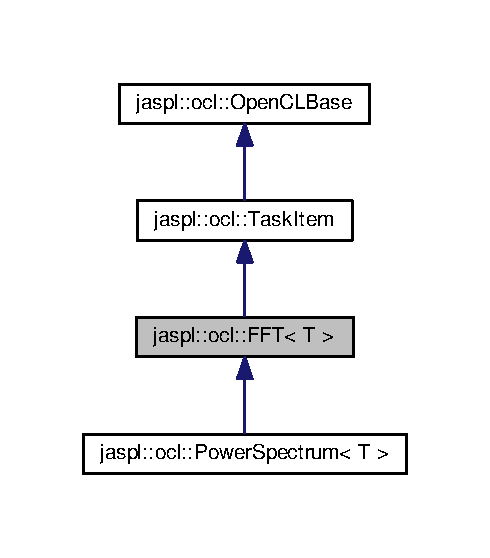
\includegraphics[width=235pt]{classjaspl_1_1ocl_1_1_f_f_t__inherit__graph}
\end{center}
\end{figure}


Collaboration diagram for jaspl\+:\+:ocl\+:\+:F\+FT$<$ T $>$\+:\nopagebreak
\begin{figure}[H]
\begin{center}
\leavevmode
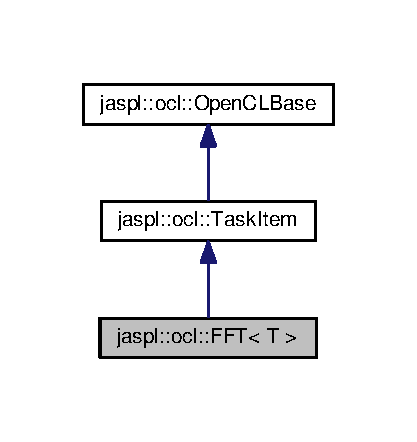
\includegraphics[width=200pt]{classjaspl_1_1ocl_1_1_f_f_t__coll__graph}
\end{center}
\end{figure}
\subsection*{Protected Member Functions}
\begin{DoxyCompactItemize}
\item 
void {\bfseries Trigger} ()\hypertarget{classjaspl_1_1ocl_1_1_f_f_t_a102a4328d7a30cc8ca8d08c907111fb2}{}\label{classjaspl_1_1ocl_1_1_f_f_t_a102a4328d7a30cc8ca8d08c907111fb2}

\item 
virtual void {\bfseries Set\+Signal} (cl\+::\+Buffer \&signal\+\_\+buff, uint sig\+\_\+size)\hypertarget{classjaspl_1_1ocl_1_1_f_f_t_ab38bdc5c38a82feaddb370f965295efd}{}\label{classjaspl_1_1ocl_1_1_f_f_t_ab38bdc5c38a82feaddb370f965295efd}

\item 
virtual cl\+::\+Buffer \& {\bfseries Processed\+Signal} ()\hypertarget{classjaspl_1_1ocl_1_1_f_f_t_aa03127efd639a389ec6869cc77fed978}{}\label{classjaspl_1_1ocl_1_1_f_f_t_aa03127efd639a389ec6869cc77fed978}

\item 
virtual size\+\_\+t {\bfseries Processed\+Signal\+Bytes} ()\hypertarget{classjaspl_1_1ocl_1_1_f_f_t_ad81ffbffde684b7d2cc68ee7b0c18e67}{}\label{classjaspl_1_1ocl_1_1_f_f_t_ad81ffbffde684b7d2cc68ee7b0c18e67}

\item 
virtual size\+\_\+t {\bfseries Processed\+Signal\+Size} ()\hypertarget{classjaspl_1_1ocl_1_1_f_f_t_a2243fd0a1e2496d51fc0b19f4b451c2d}{}\label{classjaspl_1_1ocl_1_1_f_f_t_a2243fd0a1e2496d51fc0b19f4b451c2d}

\item 
virtual bool {\bfseries Needs\+To\+Reknew} ()\hypertarget{classjaspl_1_1ocl_1_1_f_f_t_adea0ce7544d0049bfe5c39cc35cfa379}{}\label{classjaspl_1_1ocl_1_1_f_f_t_adea0ce7544d0049bfe5c39cc35cfa379}

\item 
void {\bfseries Tear\+Down} ()\hypertarget{classjaspl_1_1ocl_1_1_f_f_t_a6ad6e55ce5ca1ce4ecb280879994359a}{}\label{classjaspl_1_1ocl_1_1_f_f_t_a6ad6e55ce5ca1ce4ecb280879994359a}

\end{DoxyCompactItemize}
\subsection*{Protected Attributes}
\begin{DoxyCompactItemize}
\item 
cl\+::\+Buffer {\bfseries local\+\_\+buff}\hypertarget{classjaspl_1_1ocl_1_1_f_f_t_a98f39cb75f2d5676c1ffb82c0006422a}{}\label{classjaspl_1_1ocl_1_1_f_f_t_a98f39cb75f2d5676c1ffb82c0006422a}

\item 
cl\+\_\+int {\bfseries err}\hypertarget{classjaspl_1_1ocl_1_1_f_f_t_a95822ff6ad0e6fa90f03f69794f2c650}{}\label{classjaspl_1_1ocl_1_1_f_f_t_a95822ff6ad0e6fa90f03f69794f2c650}

\item 
clfft\+Plan\+Handle {\bfseries plan\+Handle}\hypertarget{classjaspl_1_1ocl_1_1_f_f_t_aaeaaa3e6875893f5c93af695a8fad890}{}\label{classjaspl_1_1ocl_1_1_f_f_t_aaeaaa3e6875893f5c93af695a8fad890}

\item 
clfft\+Setup\+Data {\bfseries fft\+Setup}\hypertarget{classjaspl_1_1ocl_1_1_f_f_t_a018175fb482ddf655703b93f147f7158}{}\label{classjaspl_1_1ocl_1_1_f_f_t_a018175fb482ddf655703b93f147f7158}

\item 
clfft\+Dim {\bfseries dim} = C\+L\+F\+F\+T\+\_\+1D\hypertarget{classjaspl_1_1ocl_1_1_f_f_t_a7e10d500e11853871143a81a842b6e07}{}\label{classjaspl_1_1ocl_1_1_f_f_t_a7e10d500e11853871143a81a842b6e07}

\end{DoxyCompactItemize}
\subsection*{Additional Inherited Members}


\subsection{Detailed Description}
\subsubsection*{template$<$class T$>$\\*
class jaspl\+::ocl\+::\+F\+F\+T$<$ T $>$}



Definition at line 23 of file fft.\+h.


\hypertarget{structgnuplotio_1_1_file_handle_wrapper}{}\section{gnuplotio\+:\+:File\+Handle\+Wrapper Struct Reference}
\label{structgnuplotio_1_1_file_handle_wrapper}\index{gnuplotio\+::\+File\+Handle\+Wrapper@{gnuplotio\+::\+File\+Handle\+Wrapper}}


Inheritance diagram for gnuplotio\+:\+:File\+Handle\+Wrapper\+:
\nopagebreak
\begin{figure}[H]
\begin{center}
\leavevmode
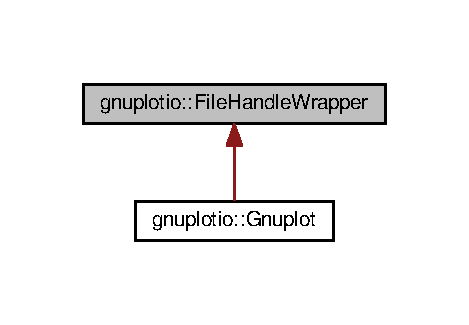
\includegraphics[width=225pt]{structgnuplotio_1_1_file_handle_wrapper__inherit__graph}
\end{center}
\end{figure}
\subsection*{Public Member Functions}
\begin{DoxyCompactItemize}
\item 
{\bfseries File\+Handle\+Wrapper} (std\+::\+F\+I\+LE $\ast$\+\_\+fh, bool \+\_\+should\+\_\+use\+\_\+pclose)\hypertarget{structgnuplotio_1_1_file_handle_wrapper_a26b2378e193a9c41be5aed97e11f9411}{}\label{structgnuplotio_1_1_file_handle_wrapper_a26b2378e193a9c41be5aed97e11f9411}

\item 
void {\bfseries fh\+\_\+close} ()\hypertarget{structgnuplotio_1_1_file_handle_wrapper_acafac45efd9c78ce621af4f3228c6f67}{}\label{structgnuplotio_1_1_file_handle_wrapper_acafac45efd9c78ce621af4f3228c6f67}

\item 
int {\bfseries fh\+\_\+fileno} ()\hypertarget{structgnuplotio_1_1_file_handle_wrapper_a3202ccd15d624f26dd2cf699d3456de6}{}\label{structgnuplotio_1_1_file_handle_wrapper_a3202ccd15d624f26dd2cf699d3456de6}

\end{DoxyCompactItemize}
\subsection*{Public Attributes}
\begin{DoxyCompactItemize}
\item 
std\+::\+F\+I\+LE $\ast$ {\bfseries wrapped\+\_\+fh}\hypertarget{structgnuplotio_1_1_file_handle_wrapper_adcb58bfcd9dbdba000a7e7395bee2ef9}{}\label{structgnuplotio_1_1_file_handle_wrapper_adcb58bfcd9dbdba000a7e7395bee2ef9}

\item 
bool {\bfseries should\+\_\+use\+\_\+pclose}\hypertarget{structgnuplotio_1_1_file_handle_wrapper_a11b63ed64cf53167e26c5273778d90ea}{}\label{structgnuplotio_1_1_file_handle_wrapper_a11b63ed64cf53167e26c5273778d90ea}

\end{DoxyCompactItemize}


\subsection{Detailed Description}


Definition at line 1523 of file gnuplot-\/iostream.\+h.


\hypertarget{structgnuplotio_1_1_flat_binary_sender}{}\section{gnuplotio\+:\+:Flat\+Binary\+Sender$<$ T $>$ Struct Template Reference}
\label{structgnuplotio_1_1_flat_binary_sender}\index{gnuplotio\+::\+Flat\+Binary\+Sender$<$ T $>$@{gnuplotio\+::\+Flat\+Binary\+Sender$<$ T $>$}}
\subsection*{Static Public Member Functions}
\begin{DoxyCompactItemize}
\item 
static void {\bfseries send} (std\+::ostream \&stream, const T \&v)\hypertarget{structgnuplotio_1_1_flat_binary_sender_a24d085492f2539c14033cd5c6ba75ba5}{}\label{structgnuplotio_1_1_flat_binary_sender_a24d085492f2539c14033cd5c6ba75ba5}

\end{DoxyCompactItemize}


\subsection{Detailed Description}
\subsubsection*{template$<$typename T$>$\\*
struct gnuplotio\+::\+Flat\+Binary\+Sender$<$ T $>$}



Definition at line 451 of file gnuplot-\/iostream.\+h.


\hypertarget{structgnuplotio_1_1_float_text_sender}{}\section{gnuplotio\+:\+:Float\+Text\+Sender$<$ T $>$ Struct Template Reference}
\label{structgnuplotio_1_1_float_text_sender}\index{gnuplotio\+::\+Float\+Text\+Sender$<$ T $>$@{gnuplotio\+::\+Float\+Text\+Sender$<$ T $>$}}
\subsection*{Static Public Member Functions}
\begin{DoxyCompactItemize}
\item 
static void {\bfseries send} (std\+::ostream \&stream, const T \&v)\hypertarget{structgnuplotio_1_1_float_text_sender_aed6b6c3a95b1396688800d6d1f2fc299}{}\label{structgnuplotio_1_1_float_text_sender_aed6b6c3a95b1396688800d6d1f2fc299}

\end{DoxyCompactItemize}


\subsection{Detailed Description}
\subsubsection*{template$<$typename T$>$\\*
struct gnuplotio\+::\+Float\+Text\+Sender$<$ T $>$}



Definition at line 505 of file gnuplot-\/iostream.\+h.


\hypertarget{classgnuplotio_1_1_gnuplot}{}\section{gnuplotio\+:\+:Gnuplot Class Reference}
\label{classgnuplotio_1_1_gnuplot}\index{gnuplotio\+::\+Gnuplot@{gnuplotio\+::\+Gnuplot}}
Inheritance diagram for gnuplotio\+:\+:Gnuplot\+:\begin{figure}[H]
\begin{center}
\leavevmode
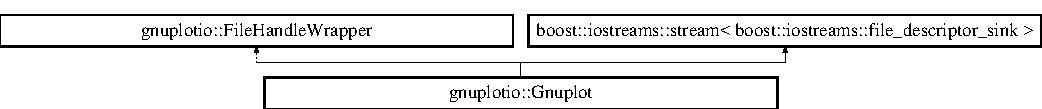
\includegraphics[height=1.469816cm]{classgnuplotio_1_1_gnuplot}
\end{center}
\end{figure}
\subsection*{Public Member Functions}
\begin{DoxyCompactItemize}
\item 
{\bfseries Gnuplot} (const std\+::string \&\+\_\+cmd=\char`\"{}\char`\"{})\hypertarget{classgnuplotio_1_1_gnuplot_ab2fb14389ab63ad5d9b2e57169bbbf1d}{}\label{classgnuplotio_1_1_gnuplot_ab2fb14389ab63ad5d9b2e57169bbbf1d}

\item 
{\bfseries Gnuplot} (F\+I\+LE $\ast$\+\_\+fh)\hypertarget{classgnuplotio_1_1_gnuplot_a4a4f48a548e6ce6d485ca0a868410078}{}\label{classgnuplotio_1_1_gnuplot_a4a4f48a548e6ce6d485ca0a868410078}

\item 
void {\bfseries clear\+Tmpfiles} ()\hypertarget{classgnuplotio_1_1_gnuplot_a0d62f80988c3db4413a668e366406393}{}\label{classgnuplotio_1_1_gnuplot_a0d62f80988c3db4413a668e366406393}

\item 
{\footnotesize template$<$typename T , typename Organization\+Mode $>$ }\\\hyperlink{classgnuplotio_1_1_gnuplot}{Gnuplot} \& {\bfseries send} (const T \&arg, Organization\+Mode)\hypertarget{classgnuplotio_1_1_gnuplot_ae3f4c07960aa5601cc72158be67f945c}{}\label{classgnuplotio_1_1_gnuplot_ae3f4c07960aa5601cc72158be67f945c}

\item 
{\footnotesize template$<$typename T , typename Organization\+Mode $>$ }\\\hyperlink{classgnuplotio_1_1_gnuplot}{Gnuplot} \& {\bfseries send\+Binary} (const T \&arg, Organization\+Mode)\hypertarget{classgnuplotio_1_1_gnuplot_a46c9e01d2030768cd811d2e8dbd10dfa}{}\label{classgnuplotio_1_1_gnuplot_a46c9e01d2030768cd811d2e8dbd10dfa}

\item 
{\footnotesize template$<$typename T , typename Organization\+Mode $>$ }\\std\+::string {\bfseries binfmt} (const T \&arg, const std\+::string \&arr\+\_\+or\+\_\+rec, Organization\+Mode)\hypertarget{classgnuplotio_1_1_gnuplot_a43fe103649ec168b453c43aecdacce81}{}\label{classgnuplotio_1_1_gnuplot_a43fe103649ec168b453c43aecdacce81}

\item 
{\footnotesize template$<$typename T , typename Organization\+Mode $>$ }\\std\+::string {\bfseries file} (const T \&arg, std\+::string filename, Organization\+Mode)\hypertarget{classgnuplotio_1_1_gnuplot_a9b9980e3b3d7cbb233a989e27468fa55}{}\label{classgnuplotio_1_1_gnuplot_a9b9980e3b3d7cbb233a989e27468fa55}

\item 
{\footnotesize template$<$typename T , typename Organization\+Mode $>$ }\\std\+::string {\bfseries binary\+File} (const T \&arg, std\+::string filename, const std\+::string \&arr\+\_\+or\+\_\+rec, Organization\+Mode)\hypertarget{classgnuplotio_1_1_gnuplot_ad90501e6dbab5379abcd76fd0e2e4ef1}{}\label{classgnuplotio_1_1_gnuplot_ad90501e6dbab5379abcd76fd0e2e4ef1}

\item 
{\footnotesize template$<$typename T $>$ }\\\hyperlink{classgnuplotio_1_1_gnuplot}{Gnuplot} {\bfseries G\+N\+U\+P\+L\+O\+T\+\_\+\+D\+E\+P\+R\+E\+C\+A\+TE} (\char`\"{}use send1d or send2d\char`\"{})\&send(const T \&arg)\hypertarget{classgnuplotio_1_1_gnuplot_ab2edc3c8f57483c6d9db86d685f3eee7}{}\label{classgnuplotio_1_1_gnuplot_ab2edc3c8f57483c6d9db86d685f3eee7}

\item 
{\footnotesize template$<$typename T $>$ }\\std\+::string {\bfseries G\+N\+U\+P\+L\+O\+T\+\_\+\+D\+E\+P\+R\+E\+C\+A\+TE} (\char`\"{}use binfmt1d or binfmt2d\char`\"{}) binfmt(const T \&arg\hypertarget{classgnuplotio_1_1_gnuplot_aeb3ba94ed04ecd46b55f89591ba23e7c}{}\label{classgnuplotio_1_1_gnuplot_aeb3ba94ed04ecd46b55f89591ba23e7c}

\end{DoxyCompactItemize}
\subsection*{Public Attributes}
\begin{DoxyCompactItemize}
\item 
std\+::string const std\+::string \& {\bfseries arr\+\_\+or\+\_\+rec}\hypertarget{classgnuplotio_1_1_gnuplot_a2d194dbd4d2f3475ff6f9b8384e62a9f}{}\label{classgnuplotio_1_1_gnuplot_a2d194dbd4d2f3475ff6f9b8384e62a9f}

\item 
std\+::vector$<$ int $>$ {\bfseries tmp\+\_\+files}\hypertarget{classgnuplotio_1_1_gnuplot_a92a4f6322e486de17db4507a5fc77348}{}\label{classgnuplotio_1_1_gnuplot_a92a4f6322e486de17db4507a5fc77348}

\item 
bool {\bfseries debug\+\_\+messages}\hypertarget{classgnuplotio_1_1_gnuplot_a63e08bfd0cd02937d895ecfb6180107c}{}\label{classgnuplotio_1_1_gnuplot_a63e08bfd0cd02937d895ecfb6180107c}

\end{DoxyCompactItemize}


\subsection{Detailed Description}


Definition at line 1551 of file gnuplot-\/iostream.\+h.


\hypertarget{classgnuplotio_1_1_gnuplot_feedback}{}\section{gnuplotio\+:\+:Gnuplot\+Feedback Class Reference}
\label{classgnuplotio_1_1_gnuplot_feedback}\index{gnuplotio\+::\+Gnuplot\+Feedback@{gnuplotio\+::\+Gnuplot\+Feedback}}
\subsection*{Public Member Functions}
\begin{DoxyCompactItemize}
\item 
virtual std\+::string {\bfseries filename} () const =0\hypertarget{classgnuplotio_1_1_gnuplot_feedback_a081d4d59ffd81e2322c07c0a802e1307}{}\label{classgnuplotio_1_1_gnuplot_feedback_a081d4d59ffd81e2322c07c0a802e1307}

\item 
virtual F\+I\+LE $\ast$ {\bfseries handle} () const =0\hypertarget{classgnuplotio_1_1_gnuplot_feedback_a13ae87ba489bfbe87f64b8b54e8a4563}{}\label{classgnuplotio_1_1_gnuplot_feedback_a13ae87ba489bfbe87f64b8b54e8a4563}

\end{DoxyCompactItemize}


\subsection{Detailed Description}


Definition at line 290 of file gnuplot-\/iostream.\+h.


\hypertarget{classjaspl_1_1has__accessor}{}\section{jaspl\+:\+:has\+\_\+accessor$<$ T $>$ Class Template Reference}
\label{classjaspl_1_1has__accessor}\index{jaspl\+::has\+\_\+accessor$<$ T $>$@{jaspl\+::has\+\_\+accessor$<$ T $>$}}
\subsection*{Public Types}
\begin{DoxyCompactItemize}
\item 
enum \{ {\bfseries value} = sizeof(test$<$T$>$(0)) == sizeof(char)
 \}\hypertarget{classjaspl_1_1has__accessor_a28163371a4d385252bfaacbed6770491}{}\label{classjaspl_1_1has__accessor_a28163371a4d385252bfaacbed6770491}

\end{DoxyCompactItemize}


\subsection{Detailed Description}
\subsubsection*{template$<$typename T$>$\\*
class jaspl\+::has\+\_\+accessor$<$ T $>$}



Definition at line 44 of file jalgorithm.\+h.


\hypertarget{structjaspl_1_1has__begin__end}{}\section{jaspl\+:\+:has\+\_\+begin\+\_\+end$<$ T $>$ Struct Template Reference}
\label{structjaspl_1_1has__begin__end}\index{jaspl\+::has\+\_\+begin\+\_\+end$<$ T $>$@{jaspl\+::has\+\_\+begin\+\_\+end$<$ T $>$}}
\subsection*{Static Public Member Functions}
\begin{DoxyCompactItemize}
\item 
{\footnotesize template$<$typename C $>$ }\\static char(\& {\bfseries f} (typename std\+::enable\+\_\+if$<$ std\+::is\+\_\+same$<$ decltype(static\+\_\+cast$<$ typename C\+::const\+\_\+iterator(C\+::$\ast$)() const  $>$(\&C\+::begin)), typename C\+::const\+\_\+iterator(C\+::$\ast$)() const  $>$\+::value, void $>$\+::type $\ast$))\mbox{[}1\mbox{]}\hypertarget{structjaspl_1_1has__begin__end_ada21a7ce698af913c3564df40dc89652}{}\label{structjaspl_1_1has__begin__end_ada21a7ce698af913c3564df40dc89652}

\item 
{\footnotesize template$<$typename C $>$ }\\static char(\& {\bfseries f} (...))\mbox{[}2\mbox{]}\hypertarget{structjaspl_1_1has__begin__end_a78807fa966c53f7ec2966588cf164038}{}\label{structjaspl_1_1has__begin__end_a78807fa966c53f7ec2966588cf164038}

\item 
{\footnotesize template$<$typename C $>$ }\\static char(\& {\bfseries g} (typename std\+::enable\+\_\+if$<$ std\+::is\+\_\+same$<$ decltype(static\+\_\+cast$<$ typename C\+::const\+\_\+iterator(C\+::$\ast$)() const  $>$(\&C\+::end)), typename C\+::const\+\_\+iterator(C\+::$\ast$)() const  $>$\+::value, void $>$\+::type $\ast$))\mbox{[}1\mbox{]}\hypertarget{structjaspl_1_1has__begin__end_ae073a73bfffe4143a11e49e9f46a362f}{}\label{structjaspl_1_1has__begin__end_ae073a73bfffe4143a11e49e9f46a362f}

\item 
{\footnotesize template$<$typename C $>$ }\\static char(\& {\bfseries g} (...))\mbox{[}2\mbox{]}\hypertarget{structjaspl_1_1has__begin__end_a4ab2cedf827f276646d35df9fd39d155}{}\label{structjaspl_1_1has__begin__end_a4ab2cedf827f276646d35df9fd39d155}

\end{DoxyCompactItemize}
\subsection*{Static Public Attributes}
\begin{DoxyCompactItemize}
\item 
static bool const {\bfseries beg\+\_\+value} = sizeof(f$<$T$>$(0)) == 1\hypertarget{structjaspl_1_1has__begin__end_a4878c9fba5b7b022c0a39cbde10e51c9}{}\label{structjaspl_1_1has__begin__end_a4878c9fba5b7b022c0a39cbde10e51c9}

\item 
static bool const {\bfseries end\+\_\+value} = sizeof(g$<$T$>$(0)) == 1\hypertarget{structjaspl_1_1has__begin__end_ac37f7ddbd100388fc793f5134d32b156}{}\label{structjaspl_1_1has__begin__end_ac37f7ddbd100388fc793f5134d32b156}

\end{DoxyCompactItemize}


\subsection{Detailed Description}
\subsubsection*{template$<$typename T$>$\\*
struct jaspl\+::has\+\_\+begin\+\_\+end$<$ T $>$}



Definition at line 195 of file jtypetraits.\+h.


\hypertarget{structjaspl_1_1has__const__iterator}{}\section{jaspl\+:\+:has\+\_\+const\+\_\+iterator$<$ T $>$ Struct Template Reference}
\label{structjaspl_1_1has__const__iterator}\index{jaspl\+::has\+\_\+const\+\_\+iterator$<$ T $>$@{jaspl\+::has\+\_\+const\+\_\+iterator$<$ T $>$}}
\subsection*{Public Types}
\begin{DoxyCompactItemize}
\item 
typedef T {\bfseries type}\hypertarget{structjaspl_1_1has__const__iterator_a90b87335124f7b6bdf7087340deb9d98}{}\label{structjaspl_1_1has__const__iterator_a90b87335124f7b6bdf7087340deb9d98}

\end{DoxyCompactItemize}
\subsection*{Static Public Attributes}
\begin{DoxyCompactItemize}
\item 
static const bool {\bfseries value} = sizeof(test$<$T$>$(0)) == sizeof(yes)\hypertarget{structjaspl_1_1has__const__iterator_aafd1712c16d8f6cccec39c5c27f0b3d3}{}\label{structjaspl_1_1has__const__iterator_aafd1712c16d8f6cccec39c5c27f0b3d3}

\end{DoxyCompactItemize}


\subsection{Detailed Description}
\subsubsection*{template$<$typename T$>$\\*
struct jaspl\+::has\+\_\+const\+\_\+iterator$<$ T $>$}



Definition at line 180 of file jtypetraits.\+h.


\hypertarget{classjaspl_1_1has__data}{}\section{jaspl\+:\+:has\+\_\+data$<$ T $>$ Class Template Reference}
\label{classjaspl_1_1has__data}\index{jaspl\+::has\+\_\+data$<$ T $>$@{jaspl\+::has\+\_\+data$<$ T $>$}}
\subsection*{Public Types}
\begin{DoxyCompactItemize}
\item 
enum \{ {\bfseries value} = sizeof(test$<$T$>$(0)) == sizeof(char)
 \}\hypertarget{classjaspl_1_1has__data_a70975109d44359f8d72c2d503fa99176}{}\label{classjaspl_1_1has__data_a70975109d44359f8d72c2d503fa99176}

\end{DoxyCompactItemize}


\subsection{Detailed Description}
\subsubsection*{template$<$typename T$>$\\*
class jaspl\+::has\+\_\+data$<$ T $>$}



Definition at line 138 of file jtypetraits.\+h.


\hypertarget{classjaspl_1_1has__data2}{}\section{jaspl\+:\+:has\+\_\+data2$<$ T, Args $>$ Class Template Reference}
\label{classjaspl_1_1has__data2}\index{jaspl\+::has\+\_\+data2$<$ T, Args $>$@{jaspl\+::has\+\_\+data2$<$ T, Args $>$}}
\subsection*{Static Public Attributes}
\begin{DoxyCompactItemize}
\item 
static constexpr bool {\bfseries value} = decltype(test$<$T$>$(0))\+::value\hypertarget{classjaspl_1_1has__data2_a5fb339475f461c83cfbc47585c1c62dc}{}\label{classjaspl_1_1has__data2_a5fb339475f461c83cfbc47585c1c62dc}

\end{DoxyCompactItemize}


\subsection{Detailed Description}
\subsubsection*{template$<$typename T, typename... Args$>$\\*
class jaspl\+::has\+\_\+data2$<$ T, Args $>$}



Definition at line 166 of file jtypetraits.\+h.


\hypertarget{classjaspl_1_1has__size}{}\section{jaspl\+:\+:has\+\_\+size$<$ T $>$ Class Template Reference}
\label{classjaspl_1_1has__size}\index{jaspl\+::has\+\_\+size$<$ T $>$@{jaspl\+::has\+\_\+size$<$ T $>$}}
\subsection*{Public Types}
\begin{DoxyCompactItemize}
\item 
enum \{ {\bfseries value} = sizeof(test$<$T$>$(0)) == sizeof(char)
 \}\hypertarget{classjaspl_1_1has__size_a8ac8f23099abf907222335e3447b6480}{}\label{classjaspl_1_1has__size_a8ac8f23099abf907222335e3447b6480}

\end{DoxyCompactItemize}


\subsection{Detailed Description}
\subsubsection*{template$<$typename T$>$\\*
class jaspl\+::has\+\_\+size$<$ T $>$}



Definition at line 152 of file jtypetraits.\+h.


\hypertarget{structgnuplotio_1_1is__boost__tuple}{}\section{gnuplotio\+:\+:is\+\_\+boost\+\_\+tuple$<$ T $>$ Struct Template Reference}
\label{structgnuplotio_1_1is__boost__tuple}\index{gnuplotio\+::is\+\_\+boost\+\_\+tuple$<$ T $>$@{gnuplotio\+::is\+\_\+boost\+\_\+tuple$<$ T $>$}}
\subsection*{Public Types}
\begin{DoxyCompactItemize}
\item 
typedef boost\+::mpl\+::and\+\_\+$<$ typename has\+\_\+head\+\_\+type$<$ T $>$\+::type, typename has\+\_\+tail\+\_\+type$<$ T $>$\+::type $>$ {\bfseries type}\hypertarget{structgnuplotio_1_1is__boost__tuple_ad771f62833b23ecae5dc689e6248396a}{}\label{structgnuplotio_1_1is__boost__tuple_ad771f62833b23ecae5dc689e6248396a}

\end{DoxyCompactItemize}
\subsection*{Static Public Attributes}
\begin{DoxyCompactItemize}
\item 
static const bool {\bfseries value} = type\+::value\hypertarget{structgnuplotio_1_1is__boost__tuple_ae6664b02421d28585204104af65a4744}{}\label{structgnuplotio_1_1is__boost__tuple_ae6664b02421d28585204104af65a4744}

\end{DoxyCompactItemize}


\subsection{Detailed Description}
\subsubsection*{template$<$typename T$>$\\*
struct gnuplotio\+::is\+\_\+boost\+\_\+tuple$<$ T $>$}



Definition at line 213 of file gnuplot-\/iostream.\+h.


\hypertarget{structgnuplotio_1_1is__boost__tuple__nulltype}{}\section{gnuplotio\+:\+:is\+\_\+boost\+\_\+tuple\+\_\+nulltype$<$ T $>$ Struct Template Reference}
\label{structgnuplotio_1_1is__boost__tuple__nulltype}\index{gnuplotio\+::is\+\_\+boost\+\_\+tuple\+\_\+nulltype$<$ T $>$@{gnuplotio\+::is\+\_\+boost\+\_\+tuple\+\_\+nulltype$<$ T $>$}}
\subsection*{Public Types}
\begin{DoxyCompactItemize}
\item 
typedef boost\+::mpl\+::bool\+\_\+$<$ value $>$ {\bfseries type}\hypertarget{structgnuplotio_1_1is__boost__tuple__nulltype_a6b9e2eaadcaa5c788131d4e9e4186349}{}\label{structgnuplotio_1_1is__boost__tuple__nulltype_a6b9e2eaadcaa5c788131d4e9e4186349}

\end{DoxyCompactItemize}
\subsection*{Static Public Attributes}
\begin{DoxyCompactItemize}
\item 
static const bool {\bfseries value} = false\hypertarget{structgnuplotio_1_1is__boost__tuple__nulltype_aed42a98e58eb94c7ba55ea7d2a8f7fd2}{}\label{structgnuplotio_1_1is__boost__tuple__nulltype_aed42a98e58eb94c7ba55ea7d2a8f7fd2}

\end{DoxyCompactItemize}


\subsection{Detailed Description}
\subsubsection*{template$<$typename T$>$\\*
struct gnuplotio\+::is\+\_\+boost\+\_\+tuple\+\_\+nulltype$<$ T $>$}



Definition at line 198 of file gnuplot-\/iostream.\+h.


\hypertarget{structgnuplotio_1_1is__boost__tuple__nulltype_3_01boost_1_1tuples_1_1null__type_01_4}{}\section{gnuplotio\+:\+:is\+\_\+boost\+\_\+tuple\+\_\+nulltype$<$ boost\+:\+:tuples\+:\+:null\+\_\+type $>$ Struct Template Reference}
\label{structgnuplotio_1_1is__boost__tuple__nulltype_3_01boost_1_1tuples_1_1null__type_01_4}\index{gnuplotio\+::is\+\_\+boost\+\_\+tuple\+\_\+nulltype$<$ boost\+::tuples\+::null\+\_\+type $>$@{gnuplotio\+::is\+\_\+boost\+\_\+tuple\+\_\+nulltype$<$ boost\+::tuples\+::null\+\_\+type $>$}}
\subsection*{Public Types}
\begin{DoxyCompactItemize}
\item 
typedef boost\+::mpl\+::bool\+\_\+$<$ value $>$ {\bfseries type}\hypertarget{structgnuplotio_1_1is__boost__tuple__nulltype_3_01boost_1_1tuples_1_1null__type_01_4_aab5c47dbae2148f1e9ed4d89f25f21fd}{}\label{structgnuplotio_1_1is__boost__tuple__nulltype_3_01boost_1_1tuples_1_1null__type_01_4_aab5c47dbae2148f1e9ed4d89f25f21fd}

\end{DoxyCompactItemize}
\subsection*{Static Public Attributes}
\begin{DoxyCompactItemize}
\item 
static const bool {\bfseries value} = true\hypertarget{structgnuplotio_1_1is__boost__tuple__nulltype_3_01boost_1_1tuples_1_1null__type_01_4_ae7fc5c63a7b01851c7ce12dbf634cfea}{}\label{structgnuplotio_1_1is__boost__tuple__nulltype_3_01boost_1_1tuples_1_1null__type_01_4_ae7fc5c63a7b01851c7ce12dbf634cfea}

\end{DoxyCompactItemize}


\subsection{Detailed Description}
\subsubsection*{template$<$$>$\\*
struct gnuplotio\+::is\+\_\+boost\+\_\+tuple\+\_\+nulltype$<$ boost\+::tuples\+::null\+\_\+type $>$}



Definition at line 204 of file gnuplot-\/iostream.\+h.


\hypertarget{structgnuplotio_1_1is__like__stl__container}{}\section{gnuplotio\+:\+:is\+\_\+like\+\_\+stl\+\_\+container$<$ T $>$ Struct Template Reference}
\label{structgnuplotio_1_1is__like__stl__container}\index{gnuplotio\+::is\+\_\+like\+\_\+stl\+\_\+container$<$ T $>$@{gnuplotio\+::is\+\_\+like\+\_\+stl\+\_\+container$<$ T $>$}}
\subsection*{Public Types}
\begin{DoxyCompactItemize}
\item 
typedef boost\+::mpl\+::and\+\_\+$<$ typename has\+\_\+value\+\_\+type$<$ T $>$\+::type, typename has\+\_\+const\+\_\+iterator$<$ T $>$\+::type, boost\+::mpl\+::not\+\_\+$<$ \hyperlink{structgnuplotio_1_1dont__treat__as__stl__container}{dont\+\_\+treat\+\_\+as\+\_\+stl\+\_\+container}$<$ T $>$ $>$ $>$ {\bfseries type}\hypertarget{structgnuplotio_1_1is__like__stl__container_a050ecfa55e896a27f86d901334f47c6a}{}\label{structgnuplotio_1_1is__like__stl__container_a050ecfa55e896a27f86d901334f47c6a}

\end{DoxyCompactItemize}
\subsection*{Static Public Attributes}
\begin{DoxyCompactItemize}
\item 
static const bool {\bfseries value} = type\+::value\hypertarget{structgnuplotio_1_1is__like__stl__container_ae4761e6e807deed732e41118c785c8a4}{}\label{structgnuplotio_1_1is__like__stl__container_ae4761e6e807deed732e41118c785c8a4}

\end{DoxyCompactItemize}


\subsection{Detailed Description}
\subsubsection*{template$<$typename T$>$\\*
struct gnuplotio\+::is\+\_\+like\+\_\+stl\+\_\+container$<$ T $>$}



Definition at line 188 of file gnuplot-\/iostream.\+h.


\hypertarget{structjaspl_1_1is__stdlib__container}{}\section{jaspl\+:\+:is\+\_\+stdlib\+\_\+container$<$ T $>$ Struct Template Reference}
\label{structjaspl_1_1is__stdlib__container}\index{jaspl\+::is\+\_\+stdlib\+\_\+container$<$ T $>$@{jaspl\+::is\+\_\+stdlib\+\_\+container$<$ T $>$}}
\subsection*{Public Types}
\begin{DoxyCompactItemize}
\item 
enum \{ {\bfseries value}
 \}\hypertarget{structjaspl_1_1is__stdlib__container_a9efc3a54a283db9f7bb0ae6400664ba8}{}\label{structjaspl_1_1is__stdlib__container_a9efc3a54a283db9f7bb0ae6400664ba8}

\end{DoxyCompactItemize}


\subsection{Detailed Description}
\subsubsection*{template$<$typename T$>$\\*
struct jaspl\+::is\+\_\+stdlib\+\_\+container$<$ T $>$}



Definition at line 215 of file jtypetraits.\+h.


\hypertarget{classgnuplotio_1_1_iterator_range}{}\section{gnuplotio\+:\+:Iterator\+Range$<$ TI, TV $>$ Class Template Reference}
\label{classgnuplotio_1_1_iterator_range}\index{gnuplotio\+::\+Iterator\+Range$<$ T\+I, T\+V $>$@{gnuplotio\+::\+Iterator\+Range$<$ T\+I, T\+V $>$}}
\subsection*{Public Types}
\begin{DoxyCompactItemize}
\item 
typedef boost\+::mpl\+::if\+\_\+c$<$ is\+\_\+container, \hyperlink{structgnuplotio_1_1_error___inappropriate_deref}{Error\+\_\+\+Inappropriate\+Deref}, TV $>$\+::type {\bfseries value\+\_\+type}\hypertarget{classgnuplotio_1_1_iterator_range_a3d997739282df372a894c586c64a0687}{}\label{classgnuplotio_1_1_iterator_range_a3d997739282df372a894c586c64a0687}

\item 
typedef \hyperlink{classgnuplotio_1_1_array_traits}{Array\+Traits}$<$ TV $>$\+::range\+\_\+type {\bfseries subiter\+\_\+type}\hypertarget{classgnuplotio_1_1_iterator_range_a566ca30462a029f6df4ef16116f99acd}{}\label{classgnuplotio_1_1_iterator_range_a566ca30462a029f6df4ef16116f99acd}

\end{DoxyCompactItemize}
\subsection*{Public Member Functions}
\begin{DoxyCompactItemize}
\item 
{\bfseries Iterator\+Range} (const TI \&\+\_\+it, const TI \&\+\_\+end)\hypertarget{classgnuplotio_1_1_iterator_range_adb89135fc292dfc5152120bc7fe6135e}{}\label{classgnuplotio_1_1_iterator_range_adb89135fc292dfc5152120bc7fe6135e}

\item 
bool {\bfseries is\+\_\+end} () const \hypertarget{classgnuplotio_1_1_iterator_range_a9146c3be94e09b6318cb0590b5816d1e}{}\label{classgnuplotio_1_1_iterator_range_a9146c3be94e09b6318cb0590b5816d1e}

\item 
void {\bfseries inc} ()\hypertarget{classgnuplotio_1_1_iterator_range_a369f392a561011f8f1c93d13fd976878}{}\label{classgnuplotio_1_1_iterator_range_a369f392a561011f8f1c93d13fd976878}

\item 
value\+\_\+type {\bfseries deref} () const \hypertarget{classgnuplotio_1_1_iterator_range_a58c90f44319ecc5efe43b80892d3b7f2}{}\label{classgnuplotio_1_1_iterator_range_a58c90f44319ecc5efe43b80892d3b7f2}

\item 
\hyperlink{structgnuplotio_1_1_error___was_not_container}{subiter\+\_\+type} {\bfseries deref\+\_\+subiter} () const \hypertarget{classgnuplotio_1_1_iterator_range_a03ee1f4e4e321d6c9676b632dcfc5969}{}\label{classgnuplotio_1_1_iterator_range_a03ee1f4e4e321d6c9676b632dcfc5969}

\end{DoxyCompactItemize}
\subsection*{Static Public Attributes}
\begin{DoxyCompactItemize}
\item 
static const bool {\bfseries is\+\_\+container} = \hyperlink{classgnuplotio_1_1_array_traits}{Array\+Traits}$<$TV$>$\+::is\+\_\+container\hypertarget{classgnuplotio_1_1_iterator_range_a3f79d84bdf18761b6e49ae54d050f8ff}{}\label{classgnuplotio_1_1_iterator_range_a3f79d84bdf18761b6e49ae54d050f8ff}

\end{DoxyCompactItemize}


\subsection{Detailed Description}
\subsubsection*{template$<$typename TI, typename TV$>$\\*
class gnuplotio\+::\+Iterator\+Range$<$ T\+I, T\+V $>$}



Definition at line 860 of file gnuplot-\/iostream.\+h.


\hypertarget{class_j_chart}{}\section{J\+Chart Class Reference}
\label{class_j_chart}\index{J\+Chart@{J\+Chart}}


Inheritance diagram for J\+Chart\+:\nopagebreak
\begin{figure}[H]
\begin{center}
\leavevmode
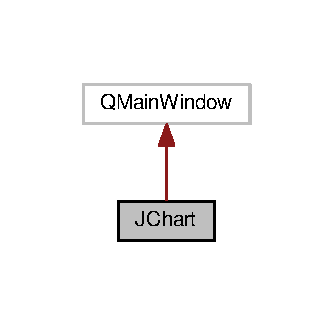
\includegraphics[width=160pt]{class_j_chart__inherit__graph}
\end{center}
\end{figure}


Collaboration diagram for J\+Chart\+:\nopagebreak
\begin{figure}[H]
\begin{center}
\leavevmode
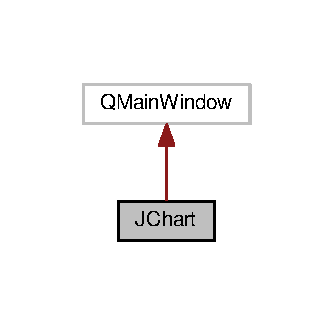
\includegraphics[width=160pt]{class_j_chart__coll__graph}
\end{center}
\end{figure}
\subsection*{Signals}
\begin{DoxyCompactItemize}
\item 
void {\bfseries Signal\+Changed} ()\hypertarget{class_j_chart_ab59324b8e03f64b90c9e414f7ff22a00}{}\label{class_j_chart_ab59324b8e03f64b90c9e414f7ff22a00}

\end{DoxyCompactItemize}
\subsection*{Public Member Functions}
\begin{DoxyCompactItemize}
\item 
{\bfseries J\+Chart} (Q\+Widget $\ast$parent=0)\hypertarget{class_j_chart_a81eedfa59e116cd9b22c10dcb94faa75}{}\label{class_j_chart_a81eedfa59e116cd9b22c10dcb94faa75}

\item 
{\footnotesize template$<$class T $>$ }\\void {\bfseries Plot} (T time\+\_\+series)\hypertarget{class_j_chart_a174b9eaf4c484e352db3ebf7d201e5a3}{}\label{class_j_chart_a174b9eaf4c484e352db3ebf7d201e5a3}

\item 
{\footnotesize template$<$class T $>$ }\\void {\bfseries Plot} (T time\+\_\+series, std\+::string chart\+\_\+title)\hypertarget{class_j_chart_a587dd3656171d836b32c4d3578066e4f}{}\label{class_j_chart_a587dd3656171d836b32c4d3578066e4f}

\end{DoxyCompactItemize}


\subsection{Detailed Description}


Definition at line 29 of file jchart.\+h.


\hypertarget{classjaspl_1_1_j_f_f_t}{}\section{jaspl\+:\+:J\+F\+FT Class Reference}
\label{classjaspl_1_1_j_f_f_t}\index{jaspl\+::\+J\+F\+FT@{jaspl\+::\+J\+F\+FT}}
\subsection*{Public Member Functions}
\begin{DoxyCompactItemize}
\item 
void {\bfseries Setup} (uint size)\hypertarget{classjaspl_1_1_j_f_f_t_a9ae772905c4f41a2de1c8b62683f6b5e}{}\label{classjaspl_1_1_j_f_f_t_a9ae772905c4f41a2de1c8b62683f6b5e}

\item 
{\footnotesize template$<$typename T $>$ }\\void {\bfseries Power\+Spectrum} (T \&input)\hypertarget{classjaspl_1_1_j_f_f_t_a3953d73759cf17cb93f2b1e76691a8fe}{}\label{classjaspl_1_1_j_f_f_t_a3953d73759cf17cb93f2b1e76691a8fe}

\item 
void {\bfseries Tear\+Down} ()\hypertarget{classjaspl_1_1_j_f_f_t_a7ba090708a0e3b6e1dba81574fa52548}{}\label{classjaspl_1_1_j_f_f_t_a7ba090708a0e3b6e1dba81574fa52548}

\end{DoxyCompactItemize}


\subsection{Detailed Description}


Definition at line 15 of file jfft.\+h.


\hypertarget{classjaspl_1_1_j_f_f_t_unit_test}{}\section{jaspl\+:\+:J\+F\+F\+T\+Unit\+Test$<$ T $>$ Class Template Reference}
\label{classjaspl_1_1_j_f_f_t_unit_test}\index{jaspl\+::\+J\+F\+F\+T\+Unit\+Test$<$ T $>$@{jaspl\+::\+J\+F\+F\+T\+Unit\+Test$<$ T $>$}}
\subsection*{Public Member Functions}
\begin{DoxyCompactItemize}
\item 
void {\bfseries Test\+C\+P\+U\+F\+FT} (uint num\+\_\+points)\hypertarget{classjaspl_1_1_j_f_f_t_unit_test_aa5c21d0d4009818fabb5aafe14fdf060}{}\label{classjaspl_1_1_j_f_f_t_unit_test_aa5c21d0d4009818fabb5aafe14fdf060}

\item 
void {\bfseries Test\+G\+P\+U\+F\+FT} (uint num\+\_\+points)\hypertarget{classjaspl_1_1_j_f_f_t_unit_test_a23b93712b332b7ec767c97473f8a73fb}{}\label{classjaspl_1_1_j_f_f_t_unit_test_a23b93712b332b7ec767c97473f8a73fb}

\end{DoxyCompactItemize}


\subsection{Detailed Description}
\subsubsection*{template$<$typename T$>$\\*
class jaspl\+::\+J\+F\+F\+T\+Unit\+Test$<$ T $>$}



Definition at line 23 of file jfft\+\_\+unit\+\_\+test.\+h.


\hypertarget{classjaspl_1_1_j_filter}{}\section{jaspl\+:\+:J\+Filter Class Reference}
\label{classjaspl_1_1_j_filter}\index{jaspl\+::\+J\+Filter@{jaspl\+::\+J\+Filter}}


\subsection{Detailed Description}


Definition at line 21 of file jlinearfilter.\+h.


\hypertarget{classjaspl_1_1j_filter_unit_test}{}\section{jaspl\+:\+:j\+Filter\+Unit\+Test$<$ T $>$ Class Template Reference}
\label{classjaspl_1_1j_filter_unit_test}\index{jaspl\+::j\+Filter\+Unit\+Test$<$ T $>$@{jaspl\+::j\+Filter\+Unit\+Test$<$ T $>$}}
\subsection*{Public Member Functions}
\begin{DoxyCompactItemize}
\item 
void {\bfseries Check\+Filter\+C\+PU} (uint num\+\_\+points)\hypertarget{classjaspl_1_1j_filter_unit_test_ad7d58b5daf92be1e51afacdb3c04419d}{}\label{classjaspl_1_1j_filter_unit_test_ad7d58b5daf92be1e51afacdb3c04419d}

\item 
void {\bfseries Check\+Filter\+G\+PU} (uint num\+\_\+points)\hypertarget{classjaspl_1_1j_filter_unit_test_a875d01230ae647f7615c96065ab41779}{}\label{classjaspl_1_1j_filter_unit_test_a875d01230ae647f7615c96065ab41779}

\end{DoxyCompactItemize}


\subsection{Detailed Description}
\subsubsection*{template$<$typename T$>$\\*
class jaspl\+::j\+Filter\+Unit\+Test$<$ T $>$}



Definition at line 25 of file jfilter\+\_\+unit\+\_\+test.\+h.


\hypertarget{class_j_non_linear_filter}{}\section{J\+Non\+Linear\+Filter Class Reference}
\label{class_j_non_linear_filter}\index{J\+Non\+Linear\+Filter@{J\+Non\+Linear\+Filter}}


\subsection{Detailed Description}


Definition at line 5 of file jnonlinearfilter.\+h.


\hypertarget{classjaspl_1_1_j_vector}{}\section{jaspl\+:\+:J\+Vector$<$ F $>$ Class Template Reference}
\label{classjaspl_1_1_j_vector}\index{jaspl\+::\+J\+Vector$<$ F $>$@{jaspl\+::\+J\+Vector$<$ F $>$}}
\subsection*{Public Member Functions}
\begin{DoxyCompactItemize}
\item 
{\bfseries J\+Vector} (std\+::string raw\+\_\+data)\hypertarget{classjaspl_1_1_j_vector_aec9bccd8f55bdb1977f02fccc7872d86}{}\label{classjaspl_1_1_j_vector_aec9bccd8f55bdb1977f02fccc7872d86}

\item 
{\bfseries J\+Vector} (std\+::vector$<$ F $>$ vec)\hypertarget{classjaspl_1_1_j_vector_ab9a8bee6860dc4ddd3c899b73de93e54}{}\label{classjaspl_1_1_j_vector_ab9a8bee6860dc4ddd3c899b73de93e54}

\item 
{\bfseries J\+Vector} (F $\ast$ptr, uint ptr\+\_\+size)\hypertarget{classjaspl_1_1_j_vector_ae3cee2406660cf6bdd73fd416ca23835}{}\label{classjaspl_1_1_j_vector_ae3cee2406660cf6bdd73fd416ca23835}

\item 
{\bfseries J\+Vector} (uint size)\hypertarget{classjaspl_1_1_j_vector_a91890a543ea9a946a56f616dd9748bcd}{}\label{classjaspl_1_1_j_vector_a91890a543ea9a946a56f616dd9748bcd}

\item 
{\bfseries J\+Vector} (uint size, F fill\+\_\+element)\hypertarget{classjaspl_1_1_j_vector_aea6660117c28bd9a787a3318f3e2c0ec}{}\label{classjaspl_1_1_j_vector_aea6660117c28bd9a787a3318f3e2c0ec}

\item 
\hyperlink{classjaspl_1_1_j_vector}{J\+Vector}$<$ F $>$ {\bfseries operator$\ast$=} (F scalar)\hypertarget{classjaspl_1_1_j_vector_a401ed55d69adaae0850b31082694313f}{}\label{classjaspl_1_1_j_vector_a401ed55d69adaae0850b31082694313f}

\item 
\hyperlink{classjaspl_1_1_j_vector}{J\+Vector}$<$ F $>$ {\bfseries operator$\ast$} (F scalar)\hypertarget{classjaspl_1_1_j_vector_a6e882f97e2c212aebe83817924633099}{}\label{classjaspl_1_1_j_vector_a6e882f97e2c212aebe83817924633099}

\item 
\hyperlink{classjaspl_1_1_j_vector}{J\+Vector}$<$ F $>$ {\bfseries operator+=} (F scalar)\hypertarget{classjaspl_1_1_j_vector_a159125c3544f643484a088391af523c4}{}\label{classjaspl_1_1_j_vector_a159125c3544f643484a088391af523c4}

\item 
void {\bfseries push\+\_\+back} (F element)\hypertarget{classjaspl_1_1_j_vector_a8906043d61595e7737c59706c9ac7643}{}\label{classjaspl_1_1_j_vector_a8906043d61595e7737c59706c9ac7643}

\item 
void {\bfseries push\+\_\+front} (F element)\hypertarget{classjaspl_1_1_j_vector_ada7d072df43b19a445f00fc7e9a36e25}{}\label{classjaspl_1_1_j_vector_ada7d072df43b19a445f00fc7e9a36e25}

\item 
std\+::vector$<$ F $>$\+::iterator {\bfseries begin} ()\hypertarget{classjaspl_1_1_j_vector_ade0638fb564d0c859abdbdc23ba97fa3}{}\label{classjaspl_1_1_j_vector_ade0638fb564d0c859abdbdc23ba97fa3}

\item 
std\+::vector$<$ F $>$\+::iterator {\bfseries end} ()\hypertarget{classjaspl_1_1_j_vector_a47d157a58ee97a0b7170f1cff4f70511}{}\label{classjaspl_1_1_j_vector_a47d157a58ee97a0b7170f1cff4f70511}

\item 
F $\ast$ {\bfseries data} ()\hypertarget{classjaspl_1_1_j_vector_ad52b5a350b0e408a9158cc4c6eba7d0f}{}\label{classjaspl_1_1_j_vector_ad52b5a350b0e408a9158cc4c6eba7d0f}

\item 
F \& {\bfseries operator\mbox{[}$\,$\mbox{]}} (const uint index)\hypertarget{classjaspl_1_1_j_vector_a077310d6ba37aa477e70bfceaa79e916}{}\label{classjaspl_1_1_j_vector_a077310d6ba37aa477e70bfceaa79e916}

\item 
F \& {\bfseries at} (const uint index)\hypertarget{classjaspl_1_1_j_vector_a199548bafdcf1f257368a27ec6243069}{}\label{classjaspl_1_1_j_vector_a199548bafdcf1f257368a27ec6243069}

\item 
void {\bfseries reserve} (uint n)\hypertarget{classjaspl_1_1_j_vector_a4d1ff6d9b08324a8db47087dc5c64efc}{}\label{classjaspl_1_1_j_vector_a4d1ff6d9b08324a8db47087dc5c64efc}

\item 
double {\bfseries norm} ()\hypertarget{classjaspl_1_1_j_vector_a7811d30c896a5411fb8e23d290437f92}{}\label{classjaspl_1_1_j_vector_a7811d30c896a5411fb8e23d290437f92}

\item 
void {\bfseries Normalize} ()\hypertarget{classjaspl_1_1_j_vector_a2144d5df7ed2c44ccd6e43aa586ec484}{}\label{classjaspl_1_1_j_vector_a2144d5df7ed2c44ccd6e43aa586ec484}

\item 
double {\bfseries std\+\_\+dev} ()\hypertarget{classjaspl_1_1_j_vector_a26ad1598c827f28aeb159f036a890c1c}{}\label{classjaspl_1_1_j_vector_a26ad1598c827f28aeb159f036a890c1c}

\item 
double {\bfseries mean} ()\hypertarget{classjaspl_1_1_j_vector_a14a30029d1e440c09f8353b0eb9f8fa0}{}\label{classjaspl_1_1_j_vector_a14a30029d1e440c09f8353b0eb9f8fa0}

\item 
F {\bfseries min} ()\hypertarget{classjaspl_1_1_j_vector_a6bb1cfc7f6c73526cc079a20994abfcd}{}\label{classjaspl_1_1_j_vector_a6bb1cfc7f6c73526cc079a20994abfcd}

\item 
F {\bfseries max} ()\hypertarget{classjaspl_1_1_j_vector_a670b6ae1e2becf0f0c311483ff7ae8b1}{}\label{classjaspl_1_1_j_vector_a670b6ae1e2becf0f0c311483ff7ae8b1}

\item 
uint {\bfseries size} ()\hypertarget{classjaspl_1_1_j_vector_a704189ad3e7f18bc6c2a42df23ce20eb}{}\label{classjaspl_1_1_j_vector_a704189ad3e7f18bc6c2a42df23ce20eb}

\end{DoxyCompactItemize}
\subsection*{Friends}
\begin{DoxyCompactItemize}
\item 
{\footnotesize template$<$class T $>$ }\\void {\bfseries plot} (\hyperlink{classjaspl_1_1_j_vector}{J\+Vector}$<$ T $>$ \&vec)\hypertarget{classjaspl_1_1_j_vector_a6dc51c5dfdd4aacdf08ebad6d0d2afae}{}\label{classjaspl_1_1_j_vector_a6dc51c5dfdd4aacdf08ebad6d0d2afae}

\item 
{\footnotesize template$<$class T $>$ }\\void {\bfseries plot} (\hyperlink{classjaspl_1_1_j_vector}{J\+Vector}$<$ T $>$ \&vec, std\+::string plot\+\_\+title)\hypertarget{classjaspl_1_1_j_vector_a61b154a38160f96e7326fa73252f59ff}{}\label{classjaspl_1_1_j_vector_a61b154a38160f96e7326fa73252f59ff}

\item 
bool {\bfseries operator==} (\hyperlink{classjaspl_1_1_j_vector}{J\+Vector}$<$ F $>$ \&vector\+\_\+a, \hyperlink{classjaspl_1_1_j_vector}{J\+Vector}$<$ F $>$ \&vector\+\_\+b)\hypertarget{classjaspl_1_1_j_vector_a81fad03b34e80d689ede7e6d7178ed56}{}\label{classjaspl_1_1_j_vector_a81fad03b34e80d689ede7e6d7178ed56}

\item 
bool {\bfseries operator!=} (\hyperlink{classjaspl_1_1_j_vector}{J\+Vector}$<$ F $>$ \&vector\+\_\+a, \hyperlink{classjaspl_1_1_j_vector}{J\+Vector}$<$ F $>$ \&vector\+\_\+b)\hypertarget{classjaspl_1_1_j_vector_ad9f0b4638213ca7ffad3c23031a58c35}{}\label{classjaspl_1_1_j_vector_ad9f0b4638213ca7ffad3c23031a58c35}

\item 
std\+::ostream \& {\bfseries operator$<$$<$} (std\+::ostream \&stream, \hyperlink{classjaspl_1_1_j_vector}{J\+Vector}$<$ F $>$ \&spectrum)\hypertarget{classjaspl_1_1_j_vector_a5bb4330c3ad441ee4a22dd90c019f20d}{}\label{classjaspl_1_1_j_vector_a5bb4330c3ad441ee4a22dd90c019f20d}

\item 
std\+::ofstream \& {\bfseries operator$<$$<$} (std\+::ofstream \&stream, \hyperlink{classjaspl_1_1_j_vector}{J\+Vector}$<$ F $>$ \&spectrum)\hypertarget{classjaspl_1_1_j_vector_aa520fbd88b8c88fc26f1d352ac911f37}{}\label{classjaspl_1_1_j_vector_aa520fbd88b8c88fc26f1d352ac911f37}

\item 
\hyperlink{classjaspl_1_1_j_vector}{J\+Vector}$<$ F $>$ {\bfseries operator+} (\hyperlink{classjaspl_1_1_j_vector}{J\+Vector}$<$ F $>$ \&vector\+\_\+a, \hyperlink{classjaspl_1_1_j_vector}{J\+Vector}$<$ F $>$ \&vector\+\_\+b)\hypertarget{classjaspl_1_1_j_vector_ab0c3db97c64f145b82254682de3a9dac}{}\label{classjaspl_1_1_j_vector_ab0c3db97c64f145b82254682de3a9dac}

\item 
\hyperlink{classjaspl_1_1_j_vector}{J\+Vector}$<$ F $>$ {\bfseries operator+} (\hyperlink{classjaspl_1_1_j_vector}{J\+Vector}$<$ F $>$ \&vector\+\_\+a, std\+::vector$<$ F $>$ \&vector\+\_\+b)\hypertarget{classjaspl_1_1_j_vector_a2d32b7256486f2427723aa03d2e21016}{}\label{classjaspl_1_1_j_vector_a2d32b7256486f2427723aa03d2e21016}

\item 
\hyperlink{classjaspl_1_1_j_vector}{J\+Vector}$<$ F $>$ {\bfseries operator-\/} (\hyperlink{classjaspl_1_1_j_vector}{J\+Vector}$<$ F $>$ \&vector\+\_\+a, \hyperlink{classjaspl_1_1_j_vector}{J\+Vector}$<$ F $>$ \&vector\+\_\+b)\hypertarget{classjaspl_1_1_j_vector_a0346f9409f8dbf1c202a587bd4be6e6d}{}\label{classjaspl_1_1_j_vector_a0346f9409f8dbf1c202a587bd4be6e6d}

\item 
\hyperlink{classjaspl_1_1_j_vector}{J\+Vector}$<$ F $>$ {\bfseries operator-\/} (\hyperlink{classjaspl_1_1_j_vector}{J\+Vector}$<$ F $>$ \&vector\+\_\+a, std\+::vector$<$ F $>$ \&vector\+\_\+b)\hypertarget{classjaspl_1_1_j_vector_ae6badaa441ef27ab6140d8dcec31eae8}{}\label{classjaspl_1_1_j_vector_ae6badaa441ef27ab6140d8dcec31eae8}

\item 
\hyperlink{classjaspl_1_1_j_vector}{J\+Vector}$<$ F $>$ {\bfseries operator$\ast$} (\hyperlink{classjaspl_1_1_j_vector}{J\+Vector}$<$ F $>$ \&vector\+\_\+a, \hyperlink{classjaspl_1_1_j_vector}{J\+Vector}$<$ F $>$ \&vector\+\_\+b)\hypertarget{classjaspl_1_1_j_vector_a2c5ea5529b0e58fd7cca8431b618d909}{}\label{classjaspl_1_1_j_vector_a2c5ea5529b0e58fd7cca8431b618d909}

\item 
\hyperlink{classjaspl_1_1_j_vector}{J\+Vector}$<$ F $>$ {\bfseries operator$\ast$} (\hyperlink{classjaspl_1_1_j_vector}{J\+Vector}$<$ F $>$ \&vector\+\_\+a, std\+::vector$<$ F $>$ \&vector\+\_\+b)\hypertarget{classjaspl_1_1_j_vector_a357e9f8d65a0e055329173fc96a269dc}{}\label{classjaspl_1_1_j_vector_a357e9f8d65a0e055329173fc96a269dc}

\end{DoxyCompactItemize}


\subsection{Detailed Description}
\subsubsection*{template$<$class F$>$\\*
class jaspl\+::\+J\+Vector$<$ F $>$}



Definition at line 20 of file jvector.\+h.


\hypertarget{classjaspl_1_1ocl_1_1_linear_convolution}{}\section{jaspl\+:\+:ocl\+:\+:Linear\+Convolution$<$ T $>$ Class Template Reference}
\label{classjaspl_1_1ocl_1_1_linear_convolution}\index{jaspl\+::ocl\+::\+Linear\+Convolution$<$ T $>$@{jaspl\+::ocl\+::\+Linear\+Convolution$<$ T $>$}}


Inheritance diagram for jaspl\+:\+:ocl\+:\+:Linear\+Convolution$<$ T $>$\+:\nopagebreak
\begin{figure}[H]
\begin{center}
\leavevmode
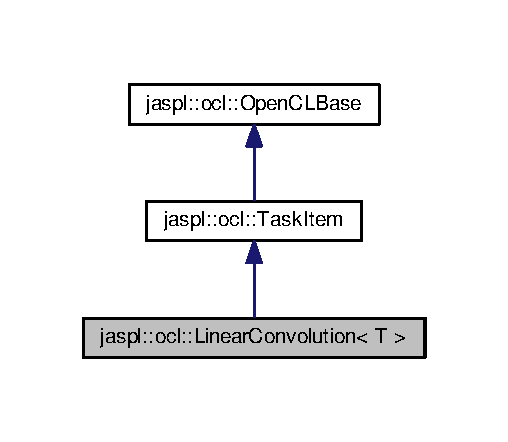
\includegraphics[width=244pt]{classjaspl_1_1ocl_1_1_linear_convolution__inherit__graph}
\end{center}
\end{figure}


Collaboration diagram for jaspl\+:\+:ocl\+:\+:Linear\+Convolution$<$ T $>$\+:\nopagebreak
\begin{figure}[H]
\begin{center}
\leavevmode
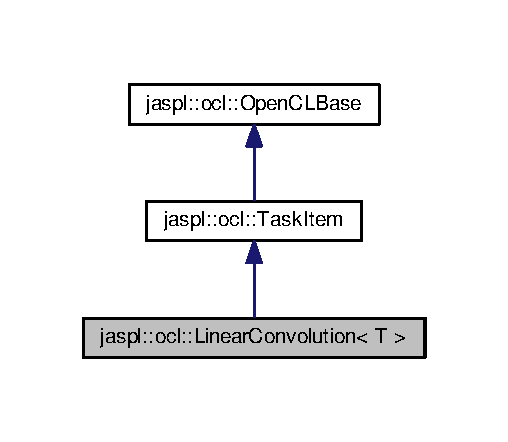
\includegraphics[width=244pt]{classjaspl_1_1ocl_1_1_linear_convolution__coll__graph}
\end{center}
\end{figure}
\subsection*{Public Member Functions}
\begin{DoxyCompactItemize}
\item 
{\bfseries Linear\+Convolution} (T \&convolution\+\_\+kernel)\hypertarget{classjaspl_1_1ocl_1_1_linear_convolution_ace2eaebe26dc0cd81332da88ecb686dd}{}\label{classjaspl_1_1ocl_1_1_linear_convolution_ace2eaebe26dc0cd81332da88ecb686dd}

\item 
{\bfseries Linear\+Convolution} (T $\ast$convolution\+\_\+kernel)\hypertarget{classjaspl_1_1ocl_1_1_linear_convolution_a24010f98b35669374fd0ac03e70a4ee2}{}\label{classjaspl_1_1ocl_1_1_linear_convolution_a24010f98b35669374fd0ac03e70a4ee2}

\end{DoxyCompactItemize}
\subsection*{Additional Inherited Members}


\subsection{Detailed Description}
\subsubsection*{template$<$class T$>$\\*
class jaspl\+::ocl\+::\+Linear\+Convolution$<$ T $>$}



Definition at line 23 of file linearconvolution.\+h.


\hypertarget{structgnuplotio_1_1_mode1_d}{}\section{gnuplotio\+:\+:Mode1D Struct Reference}
\label{structgnuplotio_1_1_mode1_d}\index{gnuplotio\+::\+Mode1D@{gnuplotio\+::\+Mode1D}}
\subsection*{Static Public Member Functions}
\begin{DoxyCompactItemize}
\item 
static std\+::string {\bfseries class\+\_\+name} ()\hypertarget{structgnuplotio_1_1_mode1_d_a508d170d84da4dfb7cd07eebad894b8f}{}\label{structgnuplotio_1_1_mode1_d_a508d170d84da4dfb7cd07eebad894b8f}

\end{DoxyCompactItemize}


\subsection{Detailed Description}


Definition at line 1207 of file gnuplot-\/iostream.\+h.


\hypertarget{structgnuplotio_1_1_mode1_d_unwrap}{}\section{gnuplotio\+:\+:Mode1\+D\+Unwrap Struct Reference}
\label{structgnuplotio_1_1_mode1_d_unwrap}\index{gnuplotio\+::\+Mode1\+D\+Unwrap@{gnuplotio\+::\+Mode1\+D\+Unwrap}}
\subsection*{Static Public Member Functions}
\begin{DoxyCompactItemize}
\item 
static std\+::string {\bfseries class\+\_\+name} ()\hypertarget{structgnuplotio_1_1_mode1_d_unwrap_a2350096ad4d8b668f6df56c32cab69b6}{}\label{structgnuplotio_1_1_mode1_d_unwrap_a2350096ad4d8b668f6df56c32cab69b6}

\end{DoxyCompactItemize}


\subsection{Detailed Description}


Definition at line 1209 of file gnuplot-\/iostream.\+h.


\hypertarget{structgnuplotio_1_1_mode2_d}{}\section{gnuplotio\+:\+:Mode2D Struct Reference}
\label{structgnuplotio_1_1_mode2_d}\index{gnuplotio\+::\+Mode2D@{gnuplotio\+::\+Mode2D}}
\subsection*{Static Public Member Functions}
\begin{DoxyCompactItemize}
\item 
static std\+::string {\bfseries class\+\_\+name} ()\hypertarget{structgnuplotio_1_1_mode2_d_aaf35c9cd117de8bc5dbc2d5ec1224232}{}\label{structgnuplotio_1_1_mode2_d_aaf35c9cd117de8bc5dbc2d5ec1224232}

\end{DoxyCompactItemize}


\subsection{Detailed Description}


Definition at line 1208 of file gnuplot-\/iostream.\+h.


\hypertarget{structgnuplotio_1_1_mode2_d_unwrap}{}\section{gnuplotio\+:\+:Mode2\+D\+Unwrap Struct Reference}
\label{structgnuplotio_1_1_mode2_d_unwrap}\index{gnuplotio\+::\+Mode2\+D\+Unwrap@{gnuplotio\+::\+Mode2\+D\+Unwrap}}
\subsection*{Static Public Member Functions}
\begin{DoxyCompactItemize}
\item 
static std\+::string {\bfseries class\+\_\+name} ()\hypertarget{structgnuplotio_1_1_mode2_d_unwrap_ab2f533c9ceb52cfecaa161c64316deb9}{}\label{structgnuplotio_1_1_mode2_d_unwrap_ab2f533c9ceb52cfecaa161c64316deb9}

\end{DoxyCompactItemize}


\subsection{Detailed Description}


Definition at line 1210 of file gnuplot-\/iostream.\+h.


\hypertarget{structgnuplotio_1_1_mode_auto}{}\section{gnuplotio\+:\+:Mode\+Auto Struct Reference}
\label{structgnuplotio_1_1_mode_auto}\index{gnuplotio\+::\+Mode\+Auto@{gnuplotio\+::\+Mode\+Auto}}
\subsection*{Static Public Member Functions}
\begin{DoxyCompactItemize}
\item 
static std\+::string {\bfseries class\+\_\+name} ()\hypertarget{structgnuplotio_1_1_mode_auto_ac73f89a782ac32dd8bc7b8f7a7581523}{}\label{structgnuplotio_1_1_mode_auto_ac73f89a782ac32dd8bc7b8f7a7581523}

\end{DoxyCompactItemize}


\subsection{Detailed Description}


Definition at line 1212 of file gnuplot-\/iostream.\+h.


\hypertarget{structgnuplotio_1_1_mode_auto_decoder}{}\section{gnuplotio\+:\+:Mode\+Auto\+Decoder$<$ T, Enable $>$ Struct Template Reference}
\label{structgnuplotio_1_1_mode_auto_decoder}\index{gnuplotio\+::\+Mode\+Auto\+Decoder$<$ T, Enable $>$@{gnuplotio\+::\+Mode\+Auto\+Decoder$<$ T, Enable $>$}}


\subsection{Detailed Description}
\subsubsection*{template$<$typename T, typename Enable = void$>$\\*
struct gnuplotio\+::\+Mode\+Auto\+Decoder$<$ T, Enable $>$}



Definition at line 1224 of file gnuplot-\/iostream.\+h.


\hypertarget{structgnuplotio_1_1_mode_binary}{}\section{gnuplotio\+:\+:Mode\+Binary Struct Reference}
\label{structgnuplotio_1_1_mode_binary}\index{gnuplotio\+::\+Mode\+Binary@{gnuplotio\+::\+Mode\+Binary}}
\subsection*{Static Public Attributes}
\begin{DoxyCompactItemize}
\item 
static const bool {\bfseries is\+\_\+text} = 0\hypertarget{structgnuplotio_1_1_mode_binary_ac89064b5df24f7ef4d765fdfde4fd1b6}{}\label{structgnuplotio_1_1_mode_binary_ac89064b5df24f7ef4d765fdfde4fd1b6}

\item 
static const bool {\bfseries is\+\_\+binfmt} = 0\hypertarget{structgnuplotio_1_1_mode_binary_aee724034dc3372b8e12b1187507bf136}{}\label{structgnuplotio_1_1_mode_binary_aee724034dc3372b8e12b1187507bf136}

\item 
static const bool {\bfseries is\+\_\+size} = 0\hypertarget{structgnuplotio_1_1_mode_binary_a6eae25ea662362bbb88bc987d6025290}{}\label{structgnuplotio_1_1_mode_binary_a6eae25ea662362bbb88bc987d6025290}

\end{DoxyCompactItemize}


\subsection{Detailed Description}


Definition at line 1196 of file gnuplot-\/iostream.\+h.


\hypertarget{structgnuplotio_1_1_mode_binfmt}{}\section{gnuplotio\+:\+:Mode\+Binfmt Struct Reference}
\label{structgnuplotio_1_1_mode_binfmt}\index{gnuplotio\+::\+Mode\+Binfmt@{gnuplotio\+::\+Mode\+Binfmt}}
\subsection*{Static Public Attributes}
\begin{DoxyCompactItemize}
\item 
static const bool {\bfseries is\+\_\+text} = 0\hypertarget{structgnuplotio_1_1_mode_binfmt_a7ab187fe922cac23b0d39ade81e5eb56}{}\label{structgnuplotio_1_1_mode_binfmt_a7ab187fe922cac23b0d39ade81e5eb56}

\item 
static const bool {\bfseries is\+\_\+binfmt} = 1\hypertarget{structgnuplotio_1_1_mode_binfmt_ab0d5d3718364cdea0347f93ec121d841}{}\label{structgnuplotio_1_1_mode_binfmt_ab0d5d3718364cdea0347f93ec121d841}

\item 
static const bool {\bfseries is\+\_\+size} = 0\hypertarget{structgnuplotio_1_1_mode_binfmt_a40a5a8ee815d6a5e9a3c30c8290a6967}{}\label{structgnuplotio_1_1_mode_binfmt_a40a5a8ee815d6a5e9a3c30c8290a6967}

\end{DoxyCompactItemize}


\subsection{Detailed Description}


Definition at line 1197 of file gnuplot-\/iostream.\+h.


\hypertarget{structgnuplotio_1_1_mode_size}{}\section{gnuplotio\+:\+:Mode\+Size Struct Reference}
\label{structgnuplotio_1_1_mode_size}\index{gnuplotio\+::\+Mode\+Size@{gnuplotio\+::\+Mode\+Size}}
\subsection*{Static Public Attributes}
\begin{DoxyCompactItemize}
\item 
static const bool {\bfseries is\+\_\+text} = 0\hypertarget{structgnuplotio_1_1_mode_size_aa01840f76877ae7c8bad254dae28e32c}{}\label{structgnuplotio_1_1_mode_size_aa01840f76877ae7c8bad254dae28e32c}

\item 
static const bool {\bfseries is\+\_\+binfmt} = 0\hypertarget{structgnuplotio_1_1_mode_size_ac5243e8e4910f2f6a2724b9fc0de4ff9}{}\label{structgnuplotio_1_1_mode_size_ac5243e8e4910f2f6a2724b9fc0de4ff9}

\item 
static const bool {\bfseries is\+\_\+size} = 1\hypertarget{structgnuplotio_1_1_mode_size_aa20ae9f1ce222504489db33d13eb46c0}{}\label{structgnuplotio_1_1_mode_size_aa20ae9f1ce222504489db33d13eb46c0}

\end{DoxyCompactItemize}


\subsection{Detailed Description}


Definition at line 1198 of file gnuplot-\/iostream.\+h.


\hypertarget{structgnuplotio_1_1_mode_text}{}\section{gnuplotio\+:\+:Mode\+Text Struct Reference}
\label{structgnuplotio_1_1_mode_text}\index{gnuplotio\+::\+Mode\+Text@{gnuplotio\+::\+Mode\+Text}}
\subsection*{Static Public Attributes}
\begin{DoxyCompactItemize}
\item 
static const bool {\bfseries is\+\_\+text} = 1\hypertarget{structgnuplotio_1_1_mode_text_a7083d8977c354a036a7c542bf99d3d52}{}\label{structgnuplotio_1_1_mode_text_a7083d8977c354a036a7c542bf99d3d52}

\item 
static const bool {\bfseries is\+\_\+binfmt} = 0\hypertarget{structgnuplotio_1_1_mode_text_a4c771363d894ae64d6af961ffde35126}{}\label{structgnuplotio_1_1_mode_text_a4c771363d894ae64d6af961ffde35126}

\item 
static const bool {\bfseries is\+\_\+size} = 0\hypertarget{structgnuplotio_1_1_mode_text_aaffc1e7bb26c6d1404cb5a3f03f13be9}{}\label{structgnuplotio_1_1_mode_text_aaffc1e7bb26c6d1404cb5a3f03f13be9}

\end{DoxyCompactItemize}


\subsection{Detailed Description}


Definition at line 1195 of file gnuplot-\/iostream.\+h.


\hypertarget{classjaspl_1_1ocl_1_1_non_linear_convolution}{}\section{jaspl\+:\+:ocl\+:\+:Non\+Linear\+Convolution$<$ T $>$ Class Template Reference}
\label{classjaspl_1_1ocl_1_1_non_linear_convolution}\index{jaspl\+::ocl\+::\+Non\+Linear\+Convolution$<$ T $>$@{jaspl\+::ocl\+::\+Non\+Linear\+Convolution$<$ T $>$}}


Inheritance diagram for jaspl\+:\+:ocl\+:\+:Non\+Linear\+Convolution$<$ T $>$\+:\nopagebreak
\begin{figure}[H]
\begin{center}
\leavevmode
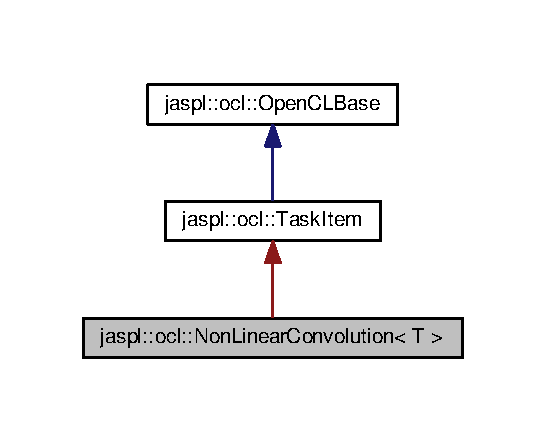
\includegraphics[width=262pt]{classjaspl_1_1ocl_1_1_non_linear_convolution__inherit__graph}
\end{center}
\end{figure}


Collaboration diagram for jaspl\+:\+:ocl\+:\+:Non\+Linear\+Convolution$<$ T $>$\+:\nopagebreak
\begin{figure}[H]
\begin{center}
\leavevmode
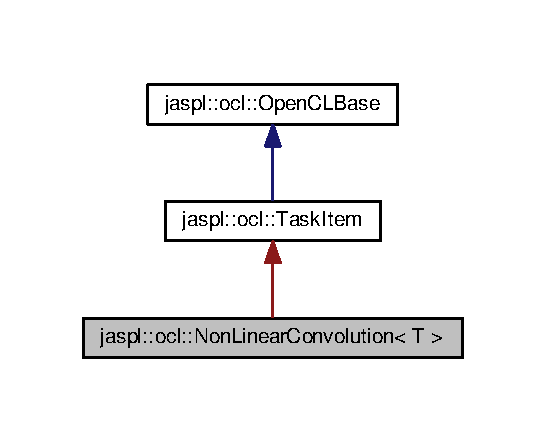
\includegraphics[width=262pt]{classjaspl_1_1ocl_1_1_non_linear_convolution__coll__graph}
\end{center}
\end{figure}
\subsection*{Public Member Functions}
\begin{DoxyCompactItemize}
\item 
{\bfseries Non\+Linear\+Convolution} (T \&convolution\+\_\+kernel)\hypertarget{classjaspl_1_1ocl_1_1_non_linear_convolution_a85fb33c4e6d02633ca25df3d3d659a3c}{}\label{classjaspl_1_1ocl_1_1_non_linear_convolution_a85fb33c4e6d02633ca25df3d3d659a3c}

\item 
{\bfseries Non\+Linear\+Convolution} (T $\ast$convolution\+\_\+kernel)\hypertarget{classjaspl_1_1ocl_1_1_non_linear_convolution_a05dfb729106ccc73d7e1d31ba5b98694}{}\label{classjaspl_1_1ocl_1_1_non_linear_convolution_a05dfb729106ccc73d7e1d31ba5b98694}

\end{DoxyCompactItemize}


\subsection{Detailed Description}
\subsubsection*{template$<$class T$>$\\*
class jaspl\+::ocl\+::\+Non\+Linear\+Convolution$<$ T $>$}



Definition at line 23 of file nonlinearconvolution.\+h.


\hypertarget{classjaspl_1_1ocl_1_1_open_c_l_base}{}\section{jaspl\+:\+:ocl\+:\+:Open\+C\+L\+Base Class Reference}
\label{classjaspl_1_1ocl_1_1_open_c_l_base}\index{jaspl\+::ocl\+::\+Open\+C\+L\+Base@{jaspl\+::ocl\+::\+Open\+C\+L\+Base}}


Base class for every class that needs access to Open\+CL Platforms, Contexts or Devices.  




{\ttfamily \#include $<$openclbase.\+h$>$}



Inheritance diagram for jaspl\+:\+:ocl\+:\+:Open\+C\+L\+Base\+:
\nopagebreak
\begin{figure}[H]
\begin{center}
\leavevmode
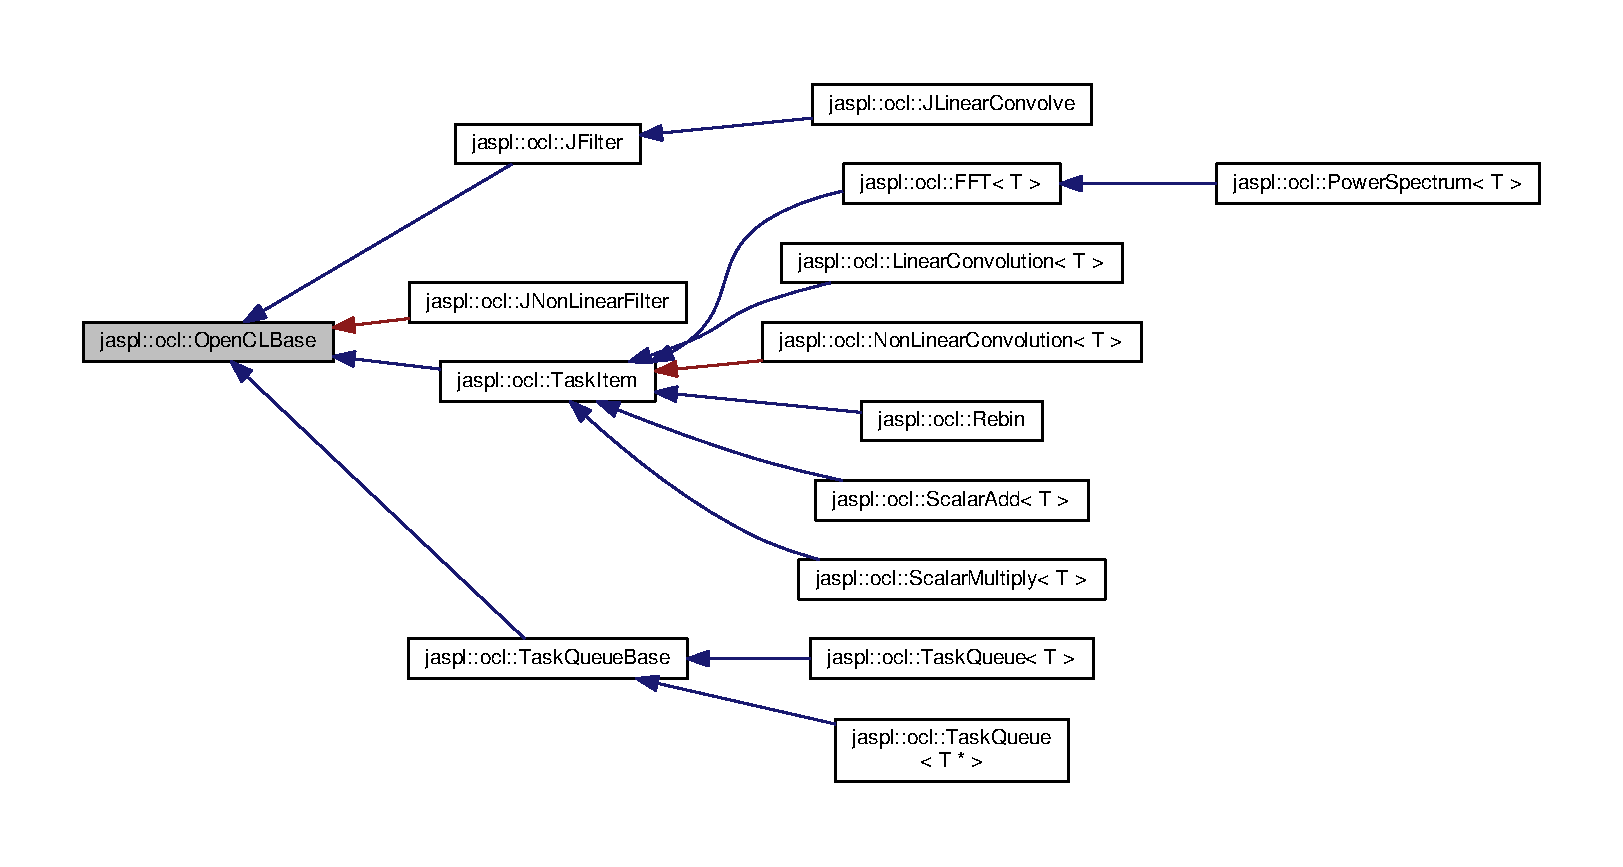
\includegraphics[width=350pt]{classjaspl_1_1ocl_1_1_open_c_l_base__inherit__graph}
\end{center}
\end{figure}
\subsection*{Public Member Functions}
\begin{DoxyCompactItemize}
\item 
\hyperlink{classjaspl_1_1ocl_1_1_open_c_l_base_a60c09a482b92e3e5fcaa488fcd391dcb}{Open\+C\+L\+Base} (uint platform\+\_\+number=0, uint device\+\_\+number=0)
\begin{DoxyCompactList}\small\item\em Initialize Open\+CL Objects Note that the Platform and Context are selected automatically\+: Platform is set to cl\+::\+Platform( 0 ) Context is set to cl\+::\+Context( device\mbox{[} device\+\_\+number \mbox{]} ) \end{DoxyCompactList}\end{DoxyCompactItemize}
\subsection*{Protected Member Functions}
\begin{DoxyCompactItemize}
\item 
void {\bfseries Set\+Up} (uint platform\+\_\+number, uint device\+\_\+number)\hypertarget{classjaspl_1_1ocl_1_1_open_c_l_base_a18031bd6b0e52aefeff4b28e98fcda96}{}\label{classjaspl_1_1ocl_1_1_open_c_l_base_a18031bd6b0e52aefeff4b28e98fcda96}

\end{DoxyCompactItemize}
\subsection*{Static Protected Attributes}
\begin{DoxyCompactItemize}
\item 
static bool {\bfseries initalized} = false\hypertarget{classjaspl_1_1ocl_1_1_open_c_l_base_ad8942a3114b511028404945d2b658689}{}\label{classjaspl_1_1ocl_1_1_open_c_l_base_ad8942a3114b511028404945d2b658689}

\item 
static std\+::vector$<$ cl\+::\+Platform $>$ {\bfseries all\+\_\+platforms}\hypertarget{classjaspl_1_1ocl_1_1_open_c_l_base_aca4e1b8a9db57208f0f4aa93053551c5}{}\label{classjaspl_1_1ocl_1_1_open_c_l_base_aca4e1b8a9db57208f0f4aa93053551c5}

\item 
static cl\+::\+Platform {\bfseries default\+\_\+platform}\hypertarget{classjaspl_1_1ocl_1_1_open_c_l_base_adba19ace68e13d2aef858d62be78305d}{}\label{classjaspl_1_1ocl_1_1_open_c_l_base_adba19ace68e13d2aef858d62be78305d}

\item 
static std\+::vector$<$ cl\+::\+Device $>$ {\bfseries all\+\_\+devices}\hypertarget{classjaspl_1_1ocl_1_1_open_c_l_base_a38970dc6296c7e86cbd2e53ed96dbf89}{}\label{classjaspl_1_1ocl_1_1_open_c_l_base_a38970dc6296c7e86cbd2e53ed96dbf89}

\item 
static cl\+::\+Device {\bfseries current\+\_\+device}\hypertarget{classjaspl_1_1ocl_1_1_open_c_l_base_ab98895e065dcdbb77e82d68fe50f3656}{}\label{classjaspl_1_1ocl_1_1_open_c_l_base_ab98895e065dcdbb77e82d68fe50f3656}

\item 
static cl\+::\+Context {\bfseries context}\hypertarget{classjaspl_1_1ocl_1_1_open_c_l_base_a630838c8c08a6bda110e04c2dda66850}{}\label{classjaspl_1_1ocl_1_1_open_c_l_base_a630838c8c08a6bda110e04c2dda66850}

\item 
static cl\+::\+Command\+Queue {\bfseries command\+\_\+queue}\hypertarget{classjaspl_1_1ocl_1_1_open_c_l_base_a96aae0bed8da50e336194b437c159e4a}{}\label{classjaspl_1_1ocl_1_1_open_c_l_base_a96aae0bed8da50e336194b437c159e4a}

\end{DoxyCompactItemize}


\subsection{Detailed Description}
Base class for every class that needs access to Open\+CL Platforms, Contexts or Devices. 

This class a common Open\+CL Platform, Context, Command\+Queue and Device for derived classes to share. 

Definition at line 31 of file openclbase.\+h.



\subsection{Constructor \& Destructor Documentation}
\index{jaspl\+::ocl\+::\+Open\+C\+L\+Base@{jaspl\+::ocl\+::\+Open\+C\+L\+Base}!Open\+C\+L\+Base@{Open\+C\+L\+Base}}
\index{Open\+C\+L\+Base@{Open\+C\+L\+Base}!jaspl\+::ocl\+::\+Open\+C\+L\+Base@{jaspl\+::ocl\+::\+Open\+C\+L\+Base}}
\subsubsection[{\texorpdfstring{Open\+C\+L\+Base(uint platform\+\_\+number=0, uint device\+\_\+number=0)}{OpenCLBase(uint platform_number=0, uint device_number=0)}}]{\setlength{\rightskip}{0pt plus 5cm}jaspl\+::ocl\+::\+Open\+C\+L\+Base\+::\+Open\+C\+L\+Base (
\begin{DoxyParamCaption}
\item[{uint}]{platform\+\_\+number = {\ttfamily 0}, }
\item[{uint}]{device\+\_\+number = {\ttfamily 0}}
\end{DoxyParamCaption}
)}\hypertarget{classjaspl_1_1ocl_1_1_open_c_l_base_a60c09a482b92e3e5fcaa488fcd391dcb}{}\label{classjaspl_1_1ocl_1_1_open_c_l_base_a60c09a482b92e3e5fcaa488fcd391dcb}


Initialize Open\+CL Objects Note that the Platform and Context are selected automatically\+: Platform is set to cl\+::\+Platform( 0 ) Context is set to cl\+::\+Context( device\mbox{[} device\+\_\+number \mbox{]} ) 

The underlying assumption is that the host machine has only one Open\+CL Platform ( e.\+g. one of A\+M\+D-\/\+A\+PP, Nvidia C\+U\+DA, Intel )


\begin{DoxyParams}{Parameters}
{\em device\+\_\+number} & Number of the Open\+CL device to use as described by cl\+::\+Platform\+::get\+Devices(\+C\+L\+\_\+\+D\+E\+V\+I\+C\+E\+\_\+\+T\+Y\+P\+E\+\_\+\+A\+L\+L) \\
\hline
\end{DoxyParams}


Definition at line 78 of file openclbase.\+cpp.


\hypertarget{classgnuplotio_1_1_pair_of_range}{}\section{gnuplotio\+:\+:Pair\+Of\+Range$<$ RT, RU $>$ Class Template Reference}
\label{classgnuplotio_1_1_pair_of_range}\index{gnuplotio\+::\+Pair\+Of\+Range$<$ R\+T, R\+U $>$@{gnuplotio\+::\+Pair\+Of\+Range$<$ R\+T, R\+U $>$}}
\subsection*{Public Types}
\begin{DoxyCompactItemize}
\item 
typedef std\+::pair$<$ typename R\+T\+::value\+\_\+type, typename R\+U\+::value\+\_\+type $>$ {\bfseries value\+\_\+type}\hypertarget{classgnuplotio_1_1_pair_of_range_a0cc8b0cc4d9c3377c43843ed9a658eeb}{}\label{classgnuplotio_1_1_pair_of_range_a0cc8b0cc4d9c3377c43843ed9a658eeb}

\item 
typedef \hyperlink{classgnuplotio_1_1_pair_of_range}{Pair\+Of\+Range}$<$ typename R\+T\+::subiter\+\_\+type, typename R\+U\+::subiter\+\_\+type $>$ {\bfseries subiter\+\_\+type}\hypertarget{classgnuplotio_1_1_pair_of_range_a6a7bf8a5dd4ca0563eb71b1156d6cd9f}{}\label{classgnuplotio_1_1_pair_of_range_a6a7bf8a5dd4ca0563eb71b1156d6cd9f}

\end{DoxyCompactItemize}
\subsection*{Public Member Functions}
\begin{DoxyCompactItemize}
\item 
{\bfseries Pair\+Of\+Range} (const RT \&\+\_\+l, const RU \&\+\_\+r)\hypertarget{classgnuplotio_1_1_pair_of_range_a15055ed8b1c0af8febf20f5a24d7dc05}{}\label{classgnuplotio_1_1_pair_of_range_a15055ed8b1c0af8febf20f5a24d7dc05}

\item 
bool {\bfseries is\+\_\+end} () const \hypertarget{classgnuplotio_1_1_pair_of_range_a1995b2f3b4c00fa9d0b4705aac4cb3ac}{}\label{classgnuplotio_1_1_pair_of_range_a1995b2f3b4c00fa9d0b4705aac4cb3ac}

\item 
void {\bfseries inc} ()\hypertarget{classgnuplotio_1_1_pair_of_range_adbb8ab0fb9f7245262041dd20444b96a}{}\label{classgnuplotio_1_1_pair_of_range_adbb8ab0fb9f7245262041dd20444b96a}

\item 
value\+\_\+type {\bfseries deref} () const \hypertarget{classgnuplotio_1_1_pair_of_range_ab4cde941279940d87a4182706ed5d88d}{}\label{classgnuplotio_1_1_pair_of_range_ab4cde941279940d87a4182706ed5d88d}

\item 
\hyperlink{classgnuplotio_1_1_pair_of_range}{subiter\+\_\+type} {\bfseries deref\+\_\+subiter} () const \hypertarget{classgnuplotio_1_1_pair_of_range_abba540b498666a006f1e31cf0cbf24c5}{}\label{classgnuplotio_1_1_pair_of_range_abba540b498666a006f1e31cf0cbf24c5}

\end{DoxyCompactItemize}
\subsection*{Static Public Attributes}
\begin{DoxyCompactItemize}
\item 
static const bool {\bfseries is\+\_\+container} = R\+T\+::is\+\_\+container \&\& R\+U\+::is\+\_\+container\hypertarget{classgnuplotio_1_1_pair_of_range_ab49c6567f0fa6a82fa2a6245fd964659}{}\label{classgnuplotio_1_1_pair_of_range_ab49c6567f0fa6a82fa2a6245fd964659}

\end{DoxyCompactItemize}
\subsection*{Friends}
\begin{DoxyCompactItemize}
\item 
{\footnotesize template$<$typename T , typename U , typename Print\+Mode $>$ }\\void {\bfseries deref\+\_\+and\+\_\+print} (std\+::ostream \&, const \hyperlink{classgnuplotio_1_1_pair_of_range}{Pair\+Of\+Range}$<$ T, U $>$ \&, Print\+Mode)\hypertarget{classgnuplotio_1_1_pair_of_range_aada62f803432f04aff66f3c609329520}{}\label{classgnuplotio_1_1_pair_of_range_aada62f803432f04aff66f3c609329520}

\end{DoxyCompactItemize}


\subsection{Detailed Description}
\subsubsection*{template$<$typename RT, typename RU$>$\\*
class gnuplotio\+::\+Pair\+Of\+Range$<$ R\+T, R\+U $>$}



Definition at line 927 of file gnuplot-\/iostream.\+h.


\hypertarget{classgnuplotio_1_1plotting__empty__container}{}\section{gnuplotio\+:\+:plotting\+\_\+empty\+\_\+container Class Reference}
\label{classgnuplotio_1_1plotting__empty__container}\index{gnuplotio\+::plotting\+\_\+empty\+\_\+container@{gnuplotio\+::plotting\+\_\+empty\+\_\+container}}
Inheritance diagram for gnuplotio\+:\+:plotting\+\_\+empty\+\_\+container\+:\begin{figure}[H]
\begin{center}
\leavevmode
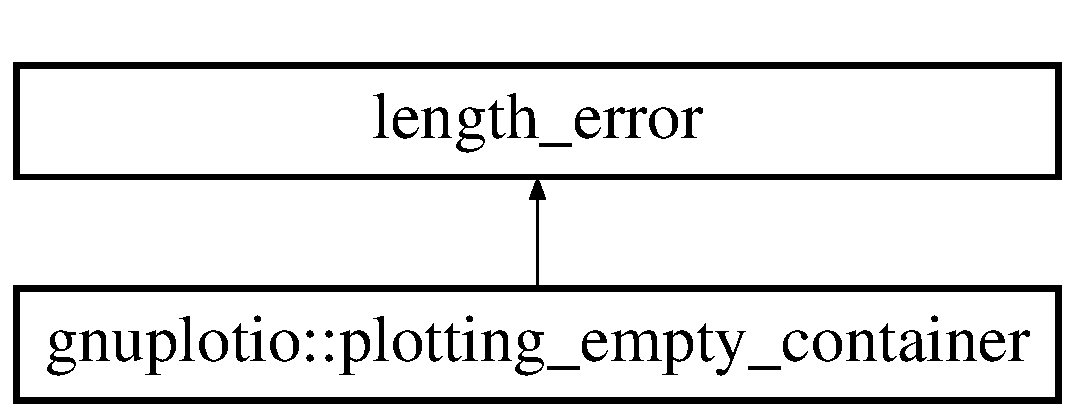
\includegraphics[height=2.000000cm]{classgnuplotio_1_1plotting__empty__container}
\end{center}
\end{figure}


\subsection{Detailed Description}


Definition at line 1180 of file gnuplot-\/iostream.\+h.


\hypertarget{classjaspl_1_1ocl_1_1_power_spectrum}{}\section{jaspl\+:\+:ocl\+:\+:Power\+Spectrum$<$ T $>$ Class Template Reference}
\label{classjaspl_1_1ocl_1_1_power_spectrum}\index{jaspl\+::ocl\+::\+Power\+Spectrum$<$ T $>$@{jaspl\+::ocl\+::\+Power\+Spectrum$<$ T $>$}}


Inheritance diagram for jaspl\+:\+:ocl\+:\+:Power\+Spectrum$<$ T $>$\+:\nopagebreak
\begin{figure}[H]
\begin{center}
\leavevmode
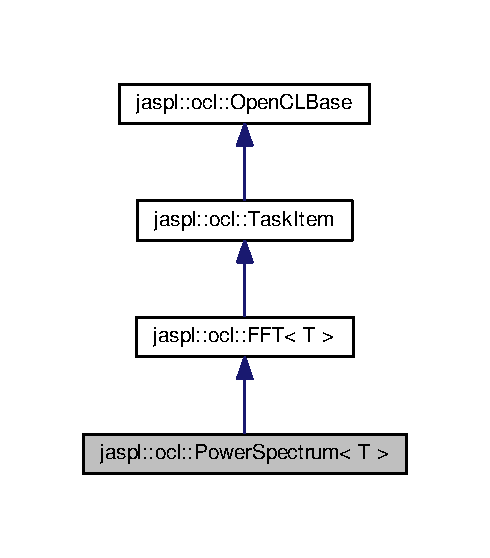
\includegraphics[width=235pt]{classjaspl_1_1ocl_1_1_power_spectrum__inherit__graph}
\end{center}
\end{figure}


Collaboration diagram for jaspl\+:\+:ocl\+:\+:Power\+Spectrum$<$ T $>$\+:\nopagebreak
\begin{figure}[H]
\begin{center}
\leavevmode
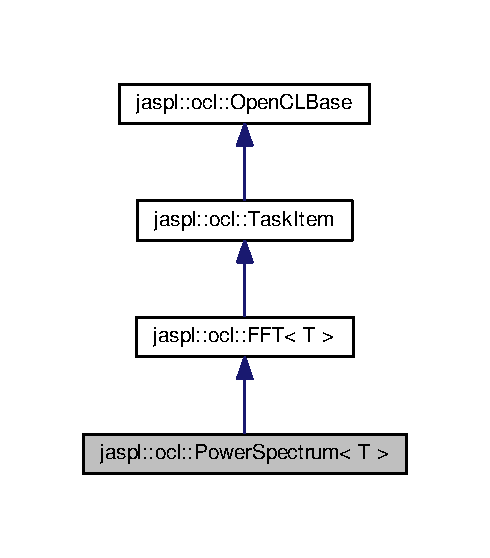
\includegraphics[width=235pt]{classjaspl_1_1ocl_1_1_power_spectrum__coll__graph}
\end{center}
\end{figure}
\subsection*{Additional Inherited Members}


\subsection{Detailed Description}
\subsubsection*{template$<$class T$>$\\*
class jaspl\+::ocl\+::\+Power\+Spectrum$<$ T $>$}



Definition at line 23 of file powerspectrum.\+h.


\hypertarget{classjaspl_1_1ocl_1_1_rebin}{}\section{jaspl\+:\+:ocl\+:\+:Rebin Class Reference}
\label{classjaspl_1_1ocl_1_1_rebin}\index{jaspl\+::ocl\+::\+Rebin@{jaspl\+::ocl\+::\+Rebin}}


Inheritance diagram for jaspl\+:\+:ocl\+:\+:Rebin\+:\nopagebreak
\begin{figure}[H]
\begin{center}
\leavevmode
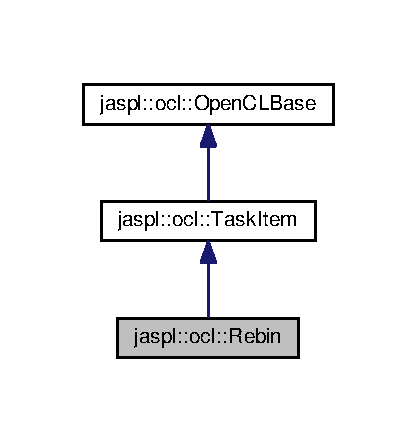
\includegraphics[width=200pt]{classjaspl_1_1ocl_1_1_rebin__inherit__graph}
\end{center}
\end{figure}


Collaboration diagram for jaspl\+:\+:ocl\+:\+:Rebin\+:\nopagebreak
\begin{figure}[H]
\begin{center}
\leavevmode
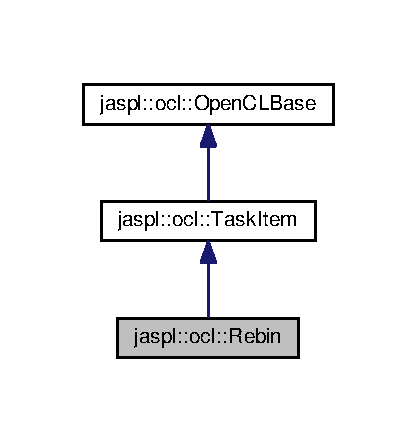
\includegraphics[width=200pt]{classjaspl_1_1ocl_1_1_rebin__coll__graph}
\end{center}
\end{figure}
\subsection*{Additional Inherited Members}


\subsection{Detailed Description}


Definition at line 21 of file rebin.\+h.


\hypertarget{classjaspl_1_1_recurse_mean}{}\section{jaspl\+:\+:Recurse\+Mean$<$ T $>$ Class Template Reference}
\label{classjaspl_1_1_recurse_mean}\index{jaspl\+::\+Recurse\+Mean$<$ T $>$@{jaspl\+::\+Recurse\+Mean$<$ T $>$}}


Average together a (nearly) arbitrary number of container-\/like objects using the recursive definition of the expected value defined by\+:  




{\ttfamily \#include $<$jalgorithm.\+h$>$}

\subsection*{Public Member Functions}
\begin{DoxyCompactItemize}
\item 
{\bfseries Recurse\+Mean} (uint num\+\_\+samples)\hypertarget{classjaspl_1_1_recurse_mean_abbcaa2624b48de1a68407cc44ca9068d}{}\label{classjaspl_1_1_recurse_mean_abbcaa2624b48de1a68407cc44ca9068d}

\item 
void \hyperlink{classjaspl_1_1_recurse_mean_a5c65990ad47245fcf866ad811cd340c3}{operator()} (const T \&next\+\_\+value)
\begin{DoxyCompactList}\small\item\em Average together a new value. \end{DoxyCompactList}\item 
void {\bfseries Reset} ()\hypertarget{classjaspl_1_1_recurse_mean_ac661dff7908c06fe1701feb7d0d07af5}{}\label{classjaspl_1_1_recurse_mean_ac661dff7908c06fe1701feb7d0d07af5}

\item 
T {\bfseries Return\+Value} ()\hypertarget{classjaspl_1_1_recurse_mean_ad9ec10f40cbfdc5f9799be43e0855572}{}\label{classjaspl_1_1_recurse_mean_ad9ec10f40cbfdc5f9799be43e0855572}

\end{DoxyCompactItemize}


\subsection{Detailed Description}
\subsubsection*{template$<$typename T$>$\\*
class jaspl\+::\+Recurse\+Mean$<$ T $>$}

Average together a (nearly) arbitrary number of container-\/like objects using the recursive definition of the expected value defined by\+: 

\[ \mu_i = \frac{ i - 1 }{ i } \mu_{ i - 1 } + \frac{1}{i} x_i\\ \text{ for } x_i \in \mathbb{R}^n \ \mu_i \in \mathcal{R} \\ \text{ and running index } i \in \mathbb{N} \]

Template parameter needs to be a container-\/liker object filled with floating-\/point values. 

Definition at line 33 of file jalgorithm.\+h.



\subsection{Member Function Documentation}
\index{jaspl\+::\+Recurse\+Mean@{jaspl\+::\+Recurse\+Mean}!operator()@{operator()}}
\index{operator()@{operator()}!jaspl\+::\+Recurse\+Mean@{jaspl\+::\+Recurse\+Mean}}
\subsubsection[{\texorpdfstring{operator()(const T \&next\+\_\+value)}{operator()(const T &next_value)}}]{\setlength{\rightskip}{0pt plus 5cm}template$<$typename T $>$ void {\bf jaspl\+::\+Recurse\+Mean}$<$ T $>$\+::operator() (
\begin{DoxyParamCaption}
\item[{const T \&}]{next\+\_\+value}
\end{DoxyParamCaption}
)}\hypertarget{classjaspl_1_1_recurse_mean_a5c65990ad47245fcf866ad811cd340c3}{}\label{classjaspl_1_1_recurse_mean_a5c65990ad47245fcf866ad811cd340c3}


Average together a new value. 


\begin{DoxyParams}{Parameters}
{\em next\+\_\+value} & The container to be averaged \\
\hline
\end{DoxyParams}

\hypertarget{classjaspl_1_1ocl_1_1_scalar_add}{}\section{jaspl\+:\+:ocl\+:\+:Scalar\+Add$<$ T $>$ Class Template Reference}
\label{classjaspl_1_1ocl_1_1_scalar_add}\index{jaspl\+::ocl\+::\+Scalar\+Add$<$ T $>$@{jaspl\+::ocl\+::\+Scalar\+Add$<$ T $>$}}


Inheritance diagram for jaspl\+:\+:ocl\+:\+:Scalar\+Add$<$ T $>$\+:\nopagebreak
\begin{figure}[H]
\begin{center}
\leavevmode
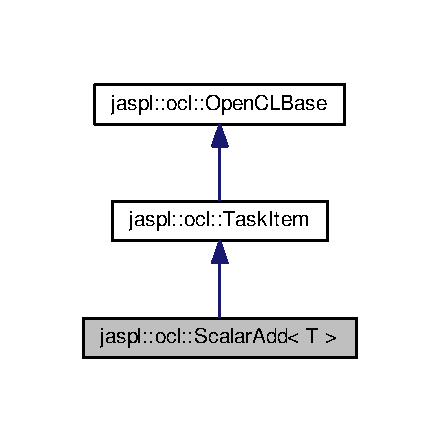
\includegraphics[width=211pt]{classjaspl_1_1ocl_1_1_scalar_add__inherit__graph}
\end{center}
\end{figure}


Collaboration diagram for jaspl\+:\+:ocl\+:\+:Scalar\+Add$<$ T $>$\+:\nopagebreak
\begin{figure}[H]
\begin{center}
\leavevmode
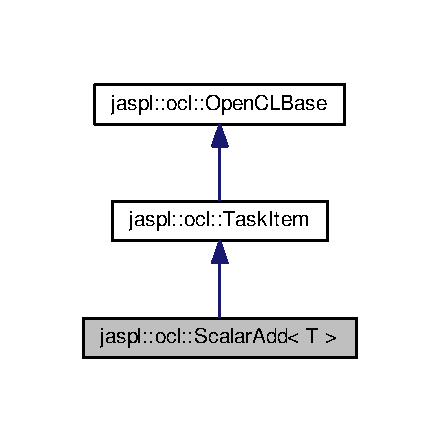
\includegraphics[width=211pt]{classjaspl_1_1ocl_1_1_scalar_add__coll__graph}
\end{center}
\end{figure}
\subsection*{Public Member Functions}
\begin{DoxyCompactItemize}
\item 
{\bfseries Scalar\+Add} (typename T\+::value\+\_\+type scalar\+\_\+value)\hypertarget{classjaspl_1_1ocl_1_1_scalar_add_a74c7684b1023fb5505afa57b65bbee2f}{}\label{classjaspl_1_1ocl_1_1_scalar_add_a74c7684b1023fb5505afa57b65bbee2f}

\end{DoxyCompactItemize}
\subsection*{Protected Member Functions}
\begin{DoxyCompactItemize}
\item 
void {\bfseries Trigger} ()\hypertarget{classjaspl_1_1ocl_1_1_scalar_add_a06f80054324b32d2a396f44e4220b061}{}\label{classjaspl_1_1ocl_1_1_scalar_add_a06f80054324b32d2a396f44e4220b061}

\item 
void {\bfseries Set\+Signal} (cl\+::\+Buffer \&signal\+\_\+buff, uint sig\+\_\+size)\hypertarget{classjaspl_1_1ocl_1_1_scalar_add_a5bb316f923cc37d6dff1144c1832decd}{}\label{classjaspl_1_1ocl_1_1_scalar_add_a5bb316f923cc37d6dff1144c1832decd}

\item 
cl\+::\+Buffer \& {\bfseries Processed\+Signal} ()\hypertarget{classjaspl_1_1ocl_1_1_scalar_add_a11727ab5b2e2c8bf8bdb8c9b8301caa0}{}\label{classjaspl_1_1ocl_1_1_scalar_add_a11727ab5b2e2c8bf8bdb8c9b8301caa0}

\item 
size\+\_\+t {\bfseries Processed\+Signal\+Bytes} ()\hypertarget{classjaspl_1_1ocl_1_1_scalar_add_aab31c814169b8419da653a79a150e3d2}{}\label{classjaspl_1_1ocl_1_1_scalar_add_aab31c814169b8419da653a79a150e3d2}

\item 
size\+\_\+t {\bfseries Processed\+Signal\+Size} ()\hypertarget{classjaspl_1_1ocl_1_1_scalar_add_a1af2d6e8f8ccf876f80afa76b9d47205}{}\label{classjaspl_1_1ocl_1_1_scalar_add_a1af2d6e8f8ccf876f80afa76b9d47205}

\item 
bool {\bfseries Needs\+To\+Reknew} ()\hypertarget{classjaspl_1_1ocl_1_1_scalar_add_abef2089f87e9d04f2d8ef4d448c7eb9b}{}\label{classjaspl_1_1ocl_1_1_scalar_add_abef2089f87e9d04f2d8ef4d448c7eb9b}

\end{DoxyCompactItemize}
\subsection*{Protected Attributes}
\begin{DoxyCompactItemize}
\item 
cl\+\_\+int {\bfseries err}\hypertarget{classjaspl_1_1ocl_1_1_scalar_add_ae5ba7922c0c238d804bc5b0e239c7d09}{}\label{classjaspl_1_1ocl_1_1_scalar_add_ae5ba7922c0c238d804bc5b0e239c7d09}

\end{DoxyCompactItemize}
\subsection*{Additional Inherited Members}


\subsection{Detailed Description}
\subsubsection*{template$<$class T$>$\\*
class jaspl\+::ocl\+::\+Scalar\+Add$<$ T $>$}



Definition at line 20 of file scalaradd.\+h.


\hypertarget{classjaspl_1_1ocl_1_1_scalar_multiply}{}\section{jaspl\+:\+:ocl\+:\+:Scalar\+Multiply$<$ T $>$ Class Template Reference}
\label{classjaspl_1_1ocl_1_1_scalar_multiply}\index{jaspl\+::ocl\+::\+Scalar\+Multiply$<$ T $>$@{jaspl\+::ocl\+::\+Scalar\+Multiply$<$ T $>$}}


Inheritance diagram for jaspl\+:\+:ocl\+:\+:Scalar\+Multiply$<$ T $>$\+:\nopagebreak
\begin{figure}[H]
\begin{center}
\leavevmode
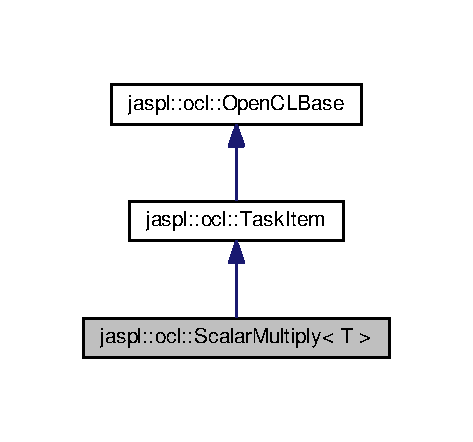
\includegraphics[width=227pt]{classjaspl_1_1ocl_1_1_scalar_multiply__inherit__graph}
\end{center}
\end{figure}


Collaboration diagram for jaspl\+:\+:ocl\+:\+:Scalar\+Multiply$<$ T $>$\+:\nopagebreak
\begin{figure}[H]
\begin{center}
\leavevmode
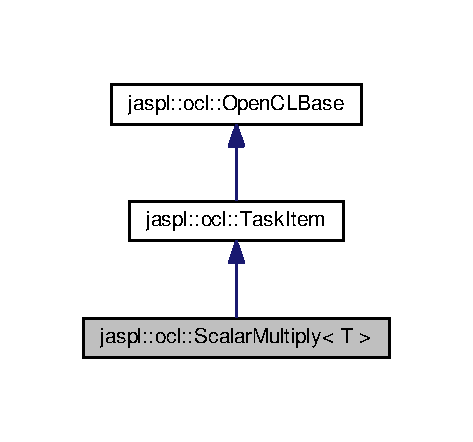
\includegraphics[width=227pt]{classjaspl_1_1ocl_1_1_scalar_multiply__coll__graph}
\end{center}
\end{figure}
\subsection*{Public Member Functions}
\begin{DoxyCompactItemize}
\item 
{\bfseries Scalar\+Multiply} (typename T\+::value\+\_\+type scalar\+\_\+value)\hypertarget{classjaspl_1_1ocl_1_1_scalar_multiply_a099a4868b984eea4d24c12c09933ee61}{}\label{classjaspl_1_1ocl_1_1_scalar_multiply_a099a4868b984eea4d24c12c09933ee61}

\end{DoxyCompactItemize}
\subsection*{Protected Member Functions}
\begin{DoxyCompactItemize}
\item 
void {\bfseries Trigger} ()\hypertarget{classjaspl_1_1ocl_1_1_scalar_multiply_a3797b44ad387b0bcd17413d11638d1c2}{}\label{classjaspl_1_1ocl_1_1_scalar_multiply_a3797b44ad387b0bcd17413d11638d1c2}

\item 
void {\bfseries Set\+Signal} (cl\+::\+Buffer \&signal\+\_\+buff, uint sig\+\_\+size)\hypertarget{classjaspl_1_1ocl_1_1_scalar_multiply_a21b27b0ec45a7327e6ddc25ea5f4d99a}{}\label{classjaspl_1_1ocl_1_1_scalar_multiply_a21b27b0ec45a7327e6ddc25ea5f4d99a}

\item 
cl\+::\+Buffer \& {\bfseries Processed\+Signal} ()\hypertarget{classjaspl_1_1ocl_1_1_scalar_multiply_acf198b3228d0b03e2c1ea12d67e387ff}{}\label{classjaspl_1_1ocl_1_1_scalar_multiply_acf198b3228d0b03e2c1ea12d67e387ff}

\item 
size\+\_\+t {\bfseries Processed\+Signal\+Bytes} ()\hypertarget{classjaspl_1_1ocl_1_1_scalar_multiply_a172e6495393f3d9b3618e471c103c95e}{}\label{classjaspl_1_1ocl_1_1_scalar_multiply_a172e6495393f3d9b3618e471c103c95e}

\item 
size\+\_\+t {\bfseries Processed\+Signal\+Size} ()\hypertarget{classjaspl_1_1ocl_1_1_scalar_multiply_ab76f39422e316fa67499cf07e8db7b4a}{}\label{classjaspl_1_1ocl_1_1_scalar_multiply_ab76f39422e316fa67499cf07e8db7b4a}

\item 
bool {\bfseries Needs\+To\+Reknew} ()\hypertarget{classjaspl_1_1ocl_1_1_scalar_multiply_a245ff6645743ee6e35d9977f68c3f70d}{}\label{classjaspl_1_1ocl_1_1_scalar_multiply_a245ff6645743ee6e35d9977f68c3f70d}

\end{DoxyCompactItemize}
\subsection*{Protected Attributes}
\begin{DoxyCompactItemize}
\item 
cl\+\_\+int {\bfseries err}\hypertarget{classjaspl_1_1ocl_1_1_scalar_multiply_a8e0f71ad2f0de06645b1f14e6ce9ec62}{}\label{classjaspl_1_1ocl_1_1_scalar_multiply_a8e0f71ad2f0de06645b1f14e6ce9ec62}

\end{DoxyCompactItemize}
\subsection*{Additional Inherited Members}


\subsection{Detailed Description}
\subsubsection*{template$<$class T$>$\\*
class jaspl\+::ocl\+::\+Scalar\+Multiply$<$ T $>$}



Definition at line 20 of file scalarmultiply.\+h.


\hypertarget{classjaspl_1_1ocl_1_1_task_item}{}\section{jaspl\+:\+:ocl\+:\+:Task\+Item Class Reference}
\label{classjaspl_1_1ocl_1_1_task_item}\index{jaspl\+::ocl\+::\+Task\+Item@{jaspl\+::ocl\+::\+Task\+Item}}


Inheritance diagram for jaspl\+:\+:ocl\+:\+:Task\+Item\+:\nopagebreak
\begin{figure}[H]
\begin{center}
\leavevmode
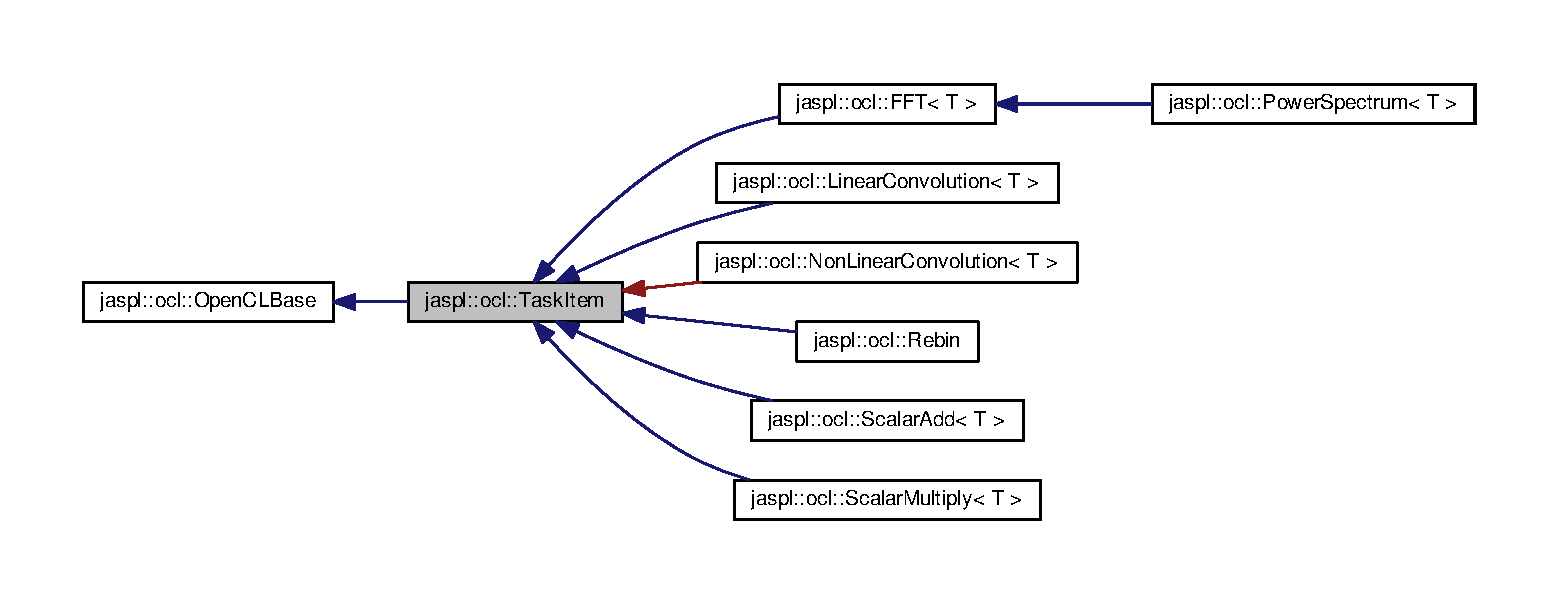
\includegraphics[width=350pt]{classjaspl_1_1ocl_1_1_task_item__inherit__graph}
\end{center}
\end{figure}


Collaboration diagram for jaspl\+:\+:ocl\+:\+:Task\+Item\+:\nopagebreak
\begin{figure}[H]
\begin{center}
\leavevmode
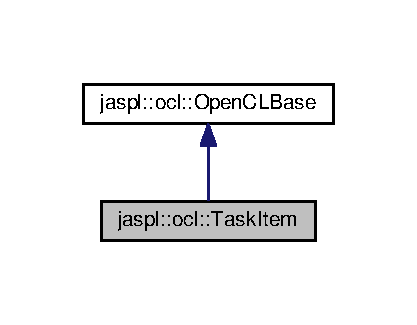
\includegraphics[width=200pt]{classjaspl_1_1ocl_1_1_task_item__coll__graph}
\end{center}
\end{figure}
\subsection*{Protected Member Functions}
\begin{DoxyCompactItemize}
\item 
{\footnotesize template$<$typename F $>$ }\\std\+::string {\bfseries Fake\+Kernel\+Templating} (std\+::string kernel\+\_\+source)\hypertarget{classjaspl_1_1ocl_1_1_task_item_aebceb791e8b1dbe70af39047d8fdae21}{}\label{classjaspl_1_1ocl_1_1_task_item_aebceb791e8b1dbe70af39047d8fdae21}

\item 
{\footnotesize template$<$typename F $>$ }\\void {\bfseries Load\+C\+L\+Kernel} (std\+::string kernel\+\_\+name)\hypertarget{classjaspl_1_1ocl_1_1_task_item_a800ffc9212ce8c25771e21b22ae867ce}{}\label{classjaspl_1_1ocl_1_1_task_item_a800ffc9212ce8c25771e21b22ae867ce}

\item 
virtual void {\bfseries Trigger} ()\hypertarget{classjaspl_1_1ocl_1_1_task_item_a186aa96ac98ce8bb8c63818e8b33e3fa}{}\label{classjaspl_1_1ocl_1_1_task_item_a186aa96ac98ce8bb8c63818e8b33e3fa}

\item 
virtual void {\bfseries Set\+Signal} (cl\+::\+Buffer \&signal\+\_\+buff, uint sig\+\_\+size)\hypertarget{classjaspl_1_1ocl_1_1_task_item_a906407a36a6dfb930b37eabaa612cea3}{}\label{classjaspl_1_1ocl_1_1_task_item_a906407a36a6dfb930b37eabaa612cea3}

\item 
virtual cl\+::\+Buffer \& {\bfseries Processed\+Signal} ()\hypertarget{classjaspl_1_1ocl_1_1_task_item_af607becf93865c5d3d8f3df6ef87f867}{}\label{classjaspl_1_1ocl_1_1_task_item_af607becf93865c5d3d8f3df6ef87f867}

\item 
virtual size\+\_\+t {\bfseries Processed\+Signal\+Bytes} ()\hypertarget{classjaspl_1_1ocl_1_1_task_item_ac82006308e53c6e42144d253bde9b535}{}\label{classjaspl_1_1ocl_1_1_task_item_ac82006308e53c6e42144d253bde9b535}

\item 
virtual size\+\_\+t {\bfseries Processed\+Signal\+Size} ()\hypertarget{classjaspl_1_1ocl_1_1_task_item_aface585662048bfa00cda3292e9d9273}{}\label{classjaspl_1_1ocl_1_1_task_item_aface585662048bfa00cda3292e9d9273}

\item 
virtual bool {\bfseries Needs\+To\+Reknew} ()\hypertarget{classjaspl_1_1ocl_1_1_task_item_a20e681f2c7b9930f99fc73ece96cb67c}{}\label{classjaspl_1_1ocl_1_1_task_item_a20e681f2c7b9930f99fc73ece96cb67c}

\item 
void {\bfseries Check\+Kernel\+Path} (std\+::string kernel\+\_\+source\+\_\+path)\hypertarget{classjaspl_1_1ocl_1_1_task_item_af048f07b953902e9ac048fb32dc86535}{}\label{classjaspl_1_1ocl_1_1_task_item_af048f07b953902e9ac048fb32dc86535}

\item 
std\+::string {\bfseries Get\+Open\+C\+L\+Source} (std\+::string kernel\+\_\+path)\hypertarget{classjaspl_1_1ocl_1_1_task_item_a015a0fc3c5fe671b6f9d529a77cb4132}{}\label{classjaspl_1_1ocl_1_1_task_item_a015a0fc3c5fe671b6f9d529a77cb4132}

\end{DoxyCompactItemize}
\subsection*{Protected Attributes}
\begin{DoxyCompactItemize}
\item 
std\+::string {\bfseries kernel\+\_\+path}\hypertarget{classjaspl_1_1ocl_1_1_task_item_aa08a1b3eaff97acd4083d81de0d78de9}{}\label{classjaspl_1_1ocl_1_1_task_item_aa08a1b3eaff97acd4083d81de0d78de9}

\item 
cl\+::\+Program\+::\+Sources {\bfseries sources}\hypertarget{classjaspl_1_1ocl_1_1_task_item_acf5a7b33791d535255f524dd7bdafa2d}{}\label{classjaspl_1_1ocl_1_1_task_item_acf5a7b33791d535255f524dd7bdafa2d}

\item 
std\+::string {\bfseries kernel\+\_\+source}\hypertarget{classjaspl_1_1ocl_1_1_task_item_a90439204dd331c6a4f488e3c6016ddfa}{}\label{classjaspl_1_1ocl_1_1_task_item_a90439204dd331c6a4f488e3c6016ddfa}

\item 
cl\+::\+Program {\bfseries program}\hypertarget{classjaspl_1_1ocl_1_1_task_item_afd9f6878a4a075d6fbc9cb2a74f3ac2e}{}\label{classjaspl_1_1ocl_1_1_task_item_afd9f6878a4a075d6fbc9cb2a74f3ac2e}

\item 
cl\+::\+Kernel {\bfseries kernel}\hypertarget{classjaspl_1_1ocl_1_1_task_item_ab628ae818420624811dee92ce68615fd}{}\label{classjaspl_1_1ocl_1_1_task_item_ab628ae818420624811dee92ce68615fd}

\item 
size\+\_\+t {\bfseries signal\+\_\+size}\hypertarget{classjaspl_1_1ocl_1_1_task_item_a8a21af3a15a0010ae139cc6b0555c380}{}\label{classjaspl_1_1ocl_1_1_task_item_a8a21af3a15a0010ae139cc6b0555c380}

\end{DoxyCompactItemize}
\subsection*{Friends}
\begin{DoxyCompactItemize}
\item 
class {\bfseries Task\+Queue\+Base}\hypertarget{classjaspl_1_1ocl_1_1_task_item_a7cef05d602ede8ae7e967835f6965bc7}{}\label{classjaspl_1_1ocl_1_1_task_item_a7cef05d602ede8ae7e967835f6965bc7}

\end{DoxyCompactItemize}
\subsection*{Additional Inherited Members}


\subsection{Detailed Description}


Definition at line 26 of file taskitem.\+h.


\hypertarget{classjaspl_1_1ocl_1_1_task_queue}{}\section{jaspl\+:\+:ocl\+:\+:Task\+Queue$<$ T $>$ Class Template Reference}
\label{classjaspl_1_1ocl_1_1_task_queue}\index{jaspl\+::ocl\+::\+Task\+Queue$<$ T $>$@{jaspl\+::ocl\+::\+Task\+Queue$<$ T $>$}}


Inheritance diagram for jaspl\+:\+:ocl\+:\+:Task\+Queue$<$ T $>$\+:\nopagebreak
\begin{figure}[H]
\begin{center}
\leavevmode
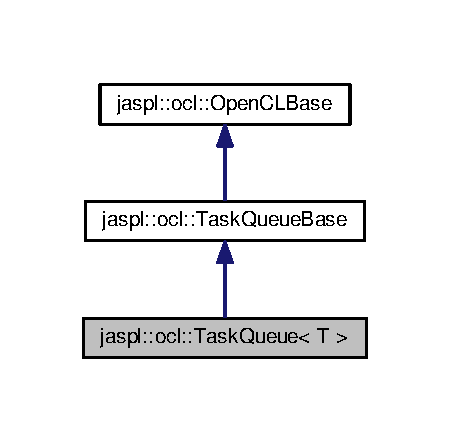
\includegraphics[width=216pt]{classjaspl_1_1ocl_1_1_task_queue__inherit__graph}
\end{center}
\end{figure}


Collaboration diagram for jaspl\+:\+:ocl\+:\+:Task\+Queue$<$ T $>$\+:\nopagebreak
\begin{figure}[H]
\begin{center}
\leavevmode
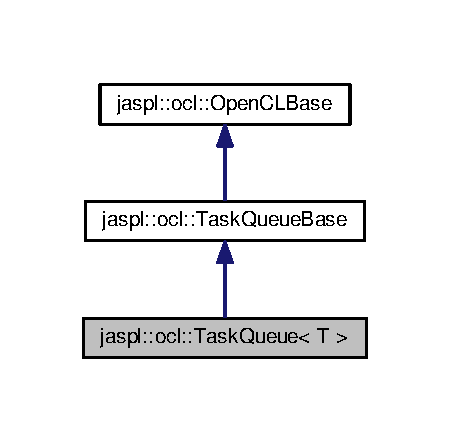
\includegraphics[width=216pt]{classjaspl_1_1ocl_1_1_task_queue__coll__graph}
\end{center}
\end{figure}
\subsection*{Public Member Functions}
\begin{DoxyCompactItemize}
\item 
{\bfseries Task\+Queue} (uint platform\+\_\+number, uint device\+\_\+number)\hypertarget{classjaspl_1_1ocl_1_1_task_queue_a622e6d731766740b8fde66c1e5dcc05d}{}\label{classjaspl_1_1ocl_1_1_task_queue_a622e6d731766740b8fde66c1e5dcc05d}

\item 
void {\bfseries Load} (T signal)\hypertarget{classjaspl_1_1ocl_1_1_task_queue_a66c6ece3e07f7eff2036bf0392606a59}{}\label{classjaspl_1_1ocl_1_1_task_queue_a66c6ece3e07f7eff2036bf0392606a59}

\item 
T {\bfseries Recall} ()\hypertarget{classjaspl_1_1ocl_1_1_task_queue_aada14bbe200a4e949cb647a20c46f22a}{}\label{classjaspl_1_1ocl_1_1_task_queue_aada14bbe200a4e949cb647a20c46f22a}

\end{DoxyCompactItemize}
\subsection*{Additional Inherited Members}


\subsection{Detailed Description}
\subsubsection*{template$<$typename T$>$\\*
class jaspl\+::ocl\+::\+Task\+Queue$<$ T $>$}



Definition at line 27 of file taskqueue.\+h.


\hypertarget{classjaspl_1_1ocl_1_1_task_queue_3_01_t_01_5_01_4}{}\section{jaspl\+:\+:ocl\+:\+:Task\+Queue$<$ T $\ast$ $>$ Class Template Reference}
\label{classjaspl_1_1ocl_1_1_task_queue_3_01_t_01_5_01_4}\index{jaspl\+::ocl\+::\+Task\+Queue$<$ T $\ast$ $>$@{jaspl\+::ocl\+::\+Task\+Queue$<$ T $\ast$ $>$}}


Inheritance diagram for jaspl\+:\+:ocl\+:\+:Task\+Queue$<$ T $\ast$ $>$\+:\nopagebreak
\begin{figure}[H]
\begin{center}
\leavevmode
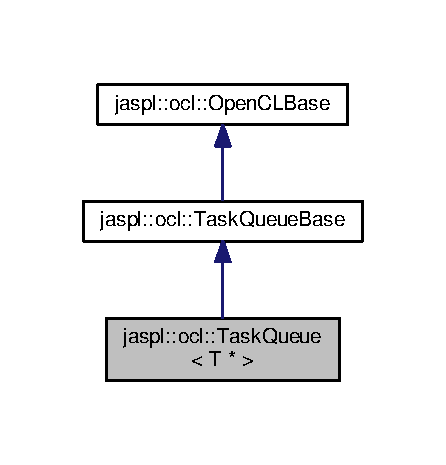
\includegraphics[width=214pt]{classjaspl_1_1ocl_1_1_task_queue_3_01_t_01_5_01_4__inherit__graph}
\end{center}
\end{figure}


Collaboration diagram for jaspl\+:\+:ocl\+:\+:Task\+Queue$<$ T $\ast$ $>$\+:\nopagebreak
\begin{figure}[H]
\begin{center}
\leavevmode
\includegraphics[width=214pt]{classjaspl_1_1ocl_1_1_task_queue_3_01_t_01_5_01_4__coll__graph}
\end{center}
\end{figure}
\subsection*{Public Member Functions}
\begin{DoxyCompactItemize}
\item 
{\bfseries Task\+Queue} (uint platform\+\_\+number, uint device\+\_\+number)\hypertarget{classjaspl_1_1ocl_1_1_task_queue_3_01_t_01_5_01_4_a79fad9fbd8502d2ad4fbc3bc72beb025}{}\label{classjaspl_1_1ocl_1_1_task_queue_3_01_t_01_5_01_4_a79fad9fbd8502d2ad4fbc3bc72beb025}

\item 
void {\bfseries Load} (T $\ast$signal\+\_\+ptr)\hypertarget{classjaspl_1_1ocl_1_1_task_queue_3_01_t_01_5_01_4_a551e195b02111e01482ef4a2783f5f1c}{}\label{classjaspl_1_1ocl_1_1_task_queue_3_01_t_01_5_01_4_a551e195b02111e01482ef4a2783f5f1c}

\item 
T $\ast$ {\bfseries Recall} ()\hypertarget{classjaspl_1_1ocl_1_1_task_queue_3_01_t_01_5_01_4_ab70f0e28df3b5b5217804a86d8f63994}{}\label{classjaspl_1_1ocl_1_1_task_queue_3_01_t_01_5_01_4_ab70f0e28df3b5b5217804a86d8f63994}

\end{DoxyCompactItemize}
\subsection*{Additional Inherited Members}


\subsection{Detailed Description}
\subsubsection*{template$<$class T$>$\\*
class jaspl\+::ocl\+::\+Task\+Queue$<$ T $\ast$ $>$}



Definition at line 39 of file taskqueue.\+h.


\hypertarget{classjaspl_1_1ocl_1_1_task_queue_base}{}\section{jaspl\+:\+:ocl\+:\+:Task\+Queue\+Base Class Reference}
\label{classjaspl_1_1ocl_1_1_task_queue_base}\index{jaspl\+::ocl\+::\+Task\+Queue\+Base@{jaspl\+::ocl\+::\+Task\+Queue\+Base}}


The fundamental structure underlying all Open\+CL Functions.  




{\ttfamily \#include $<$taskqueuebase.\+h$>$}



Inheritance diagram for jaspl\+:\+:ocl\+:\+:Task\+Queue\+Base\+:\nopagebreak
\begin{figure}[H]
\begin{center}
\leavevmode
\includegraphics[width=346pt]{classjaspl_1_1ocl_1_1_task_queue_base__inherit__graph}
\end{center}
\end{figure}


Collaboration diagram for jaspl\+:\+:ocl\+:\+:Task\+Queue\+Base\+:\nopagebreak
\begin{figure}[H]
\begin{center}
\leavevmode
\includegraphics[width=214pt]{classjaspl_1_1ocl_1_1_task_queue_base__coll__graph}
\end{center}
\end{figure}
\subsection*{Public Member Functions}
\begin{DoxyCompactItemize}
\item 
\hyperlink{classjaspl_1_1ocl_1_1_task_queue_base_a6568c5c6bd8b3d2e2ad3c13eef6fb31b}{Task\+Queue\+Base} (uint platform\+\_\+number=0, uint device\+\_\+number=0)
\begin{DoxyCompactList}\small\item\em Build a new \hyperlink{classjaspl_1_1ocl_1_1_task_queue_base}{Task\+Queue\+Base} and implicitly initialize Open\+CL Context, Platform etc. \end{DoxyCompactList}\item 
void \hyperlink{classjaspl_1_1ocl_1_1_task_queue_base_af9671abc7d62d895bb6abdd9c68bb31c}{Execute} ()
\begin{DoxyCompactList}\small\item\em Run all Task\+Items that are currently loaded. \end{DoxyCompactList}\item 
void \hyperlink{classjaspl_1_1ocl_1_1_task_queue_base_aa71fb29536edbed03a771e40b81ea741}{Add\+Task\+Item} (\hyperlink{classjaspl_1_1ocl_1_1_task_item}{Task\+Item} \&item)
\begin{DoxyCompactList}\small\item\em Add a new \hyperlink{classjaspl_1_1ocl_1_1_task_item}{Task\+Item} into the \hyperlink{classjaspl_1_1ocl_1_1_task_queue}{Task\+Queue}. \end{DoxyCompactList}\item 
bool \hyperlink{classjaspl_1_1ocl_1_1_task_queue_base_a6415d52d4baca7807b251a6534f16b69}{Remove\+Task\+Item} (\hyperlink{classjaspl_1_1ocl_1_1_task_item}{Task\+Item} \&item)
\begin{DoxyCompactList}\small\item\em Remove a \hyperlink{classjaspl_1_1ocl_1_1_task_item}{Task\+Item} from the queue (if it exists) \end{DoxyCompactList}\item 
void \hyperlink{classjaspl_1_1ocl_1_1_task_queue_base_ac548bc47ba629093eb10c3566cb55d22}{Print\+Contents} ()\hypertarget{classjaspl_1_1ocl_1_1_task_queue_base_ac548bc47ba629093eb10c3566cb55d22}{}\label{classjaspl_1_1ocl_1_1_task_queue_base_ac548bc47ba629093eb10c3566cb55d22}

\begin{DoxyCompactList}\small\item\em Print all of the current elements in the queue in the order in which they will be executed. \end{DoxyCompactList}\item 
void {\bfseries Reknew\+Signal} (cl\+::\+Buffer \&processed\+\_\+buff, size\+\_\+t processed\+\_\+bytes, size\+\_\+t processed\+\_\+size)\hypertarget{classjaspl_1_1ocl_1_1_task_queue_base_a106853a7c3e48b1446013f6769e67a8a}{}\label{classjaspl_1_1ocl_1_1_task_queue_base_a106853a7c3e48b1446013f6769e67a8a}

\end{DoxyCompactItemize}
\subsection*{Protected Attributes}
\begin{DoxyCompactItemize}
\item 
std\+::list$<$ \hyperlink{classjaspl_1_1ocl_1_1_task_item}{Task\+Item} $\ast$ $>$ {\bfseries task\+\_\+queue}\hypertarget{classjaspl_1_1ocl_1_1_task_queue_base_a62a834cd1aa09f8387685a40bbe373c6}{}\label{classjaspl_1_1ocl_1_1_task_queue_base_a62a834cd1aa09f8387685a40bbe373c6}

\item 
cl\+::\+Buffer {\bfseries signal\+\_\+input}\hypertarget{classjaspl_1_1ocl_1_1_task_queue_base_ac9d244ae1978be6bb3fc806faf99f220}{}\label{classjaspl_1_1ocl_1_1_task_queue_base_ac9d244ae1978be6bb3fc806faf99f220}

\item 
cl\+::\+Buffer {\bfseries output}\hypertarget{classjaspl_1_1ocl_1_1_task_queue_base_aefa39df1b87a263a89b91ce5de343495}{}\label{classjaspl_1_1ocl_1_1_task_queue_base_aefa39df1b87a263a89b91ce5de343495}

\item 
size\+\_\+t {\bfseries signal\+\_\+size}\hypertarget{classjaspl_1_1ocl_1_1_task_queue_base_adbcead862a33ae1a246570a7e24cf786}{}\label{classjaspl_1_1ocl_1_1_task_queue_base_adbcead862a33ae1a246570a7e24cf786}

\item 
size\+\_\+t {\bfseries signal\+\_\+bytes}\hypertarget{classjaspl_1_1ocl_1_1_task_queue_base_a1e5ba37a36ce10e34822ddf5686d2971}{}\label{classjaspl_1_1ocl_1_1_task_queue_base_a1e5ba37a36ce10e34822ddf5686d2971}

\item 
bool {\bfseries on\+\_\+device} = false\hypertarget{classjaspl_1_1ocl_1_1_task_queue_base_a30d1e5405a0eb3732756a1bb6fd97c8d}{}\label{classjaspl_1_1ocl_1_1_task_queue_base_a30d1e5405a0eb3732756a1bb6fd97c8d}

\end{DoxyCompactItemize}
\subsection*{Friends}
\begin{DoxyCompactItemize}
\item 
class {\bfseries Task\+Item}\hypertarget{classjaspl_1_1ocl_1_1_task_queue_base_aec7aa930b50aea7c2192347a80371a14}{}\label{classjaspl_1_1ocl_1_1_task_queue_base_aec7aa930b50aea7c2192347a80371a14}

\end{DoxyCompactItemize}
\subsection*{Additional Inherited Members}


\subsection{Detailed Description}
The fundamental structure underlying all Open\+CL Functions. 

Definition at line 30 of file taskqueuebase.\+h.



\subsection{Constructor \& Destructor Documentation}
\index{jaspl\+::ocl\+::\+Task\+Queue\+Base@{jaspl\+::ocl\+::\+Task\+Queue\+Base}!Task\+Queue\+Base@{Task\+Queue\+Base}}
\index{Task\+Queue\+Base@{Task\+Queue\+Base}!jaspl\+::ocl\+::\+Task\+Queue\+Base@{jaspl\+::ocl\+::\+Task\+Queue\+Base}}
\subsubsection[{\texorpdfstring{Task\+Queue\+Base(uint platform\+\_\+number=0, uint device\+\_\+number=0)}{TaskQueueBase(uint platform_number=0, uint device_number=0)}}]{\setlength{\rightskip}{0pt plus 5cm}jaspl\+::ocl\+::\+Task\+Queue\+Base\+::\+Task\+Queue\+Base (
\begin{DoxyParamCaption}
\item[{uint}]{platform\+\_\+number = {\ttfamily 0}, }
\item[{uint}]{device\+\_\+number = {\ttfamily 0}}
\end{DoxyParamCaption}
)}\hypertarget{classjaspl_1_1ocl_1_1_task_queue_base_a6568c5c6bd8b3d2e2ad3c13eef6fb31b}{}\label{classjaspl_1_1ocl_1_1_task_queue_base_a6568c5c6bd8b3d2e2ad3c13eef6fb31b}


Build a new \hyperlink{classjaspl_1_1ocl_1_1_task_queue_base}{Task\+Queue\+Base} and implicitly initialize Open\+CL Context, Platform etc. 


\begin{DoxyParams}{Parameters}
{\em device\+\_\+number} & Number of the Open\+CL device to use as described by cl\+::\+Platform\+::get\+Devices(\+C\+L\+\_\+\+D\+E\+V\+I\+C\+E\+\_\+\+T\+Y\+P\+E\+\_\+\+A\+L\+L)\\
\hline
\end{DoxyParams}
Note that this will be the device that every \hyperlink{classjaspl_1_1ocl_1_1_task_item}{Task\+Item} will be executed on. 

Definition at line 18 of file taskqueuebase.\+cpp.



\subsection{Member Function Documentation}
\index{jaspl\+::ocl\+::\+Task\+Queue\+Base@{jaspl\+::ocl\+::\+Task\+Queue\+Base}!Add\+Task\+Item@{Add\+Task\+Item}}
\index{Add\+Task\+Item@{Add\+Task\+Item}!jaspl\+::ocl\+::\+Task\+Queue\+Base@{jaspl\+::ocl\+::\+Task\+Queue\+Base}}
\subsubsection[{\texorpdfstring{Add\+Task\+Item(\+Task\+Item \&item)}{AddTaskItem(TaskItem &item)}}]{\setlength{\rightskip}{0pt plus 5cm}void jaspl\+::ocl\+::\+Task\+Queue\+Base\+::\+Add\+Task\+Item (
\begin{DoxyParamCaption}
\item[{{\bf Task\+Item} \&}]{item}
\end{DoxyParamCaption}
)}\hypertarget{classjaspl_1_1ocl_1_1_task_queue_base_aa71fb29536edbed03a771e40b81ea741}{}\label{classjaspl_1_1ocl_1_1_task_queue_base_aa71fb29536edbed03a771e40b81ea741}


Add a new \hyperlink{classjaspl_1_1ocl_1_1_task_item}{Task\+Item} into the \hyperlink{classjaspl_1_1ocl_1_1_task_queue}{Task\+Queue}. 

Items added to the queue need not be unique, repeated Task\+Items are allowed.


\begin{DoxyParams}{Parameters}
{\em item} & The \hyperlink{classjaspl_1_1ocl_1_1_task_item}{Task\+Item} to be inserted into the queue. \\
\hline
\end{DoxyParams}


Definition at line 42 of file taskqueuebase.\+cpp.

\index{jaspl\+::ocl\+::\+Task\+Queue\+Base@{jaspl\+::ocl\+::\+Task\+Queue\+Base}!Execute@{Execute}}
\index{Execute@{Execute}!jaspl\+::ocl\+::\+Task\+Queue\+Base@{jaspl\+::ocl\+::\+Task\+Queue\+Base}}
\subsubsection[{\texorpdfstring{Execute()}{Execute()}}]{\setlength{\rightskip}{0pt plus 5cm}void jaspl\+::ocl\+::\+Task\+Queue\+Base\+::\+Execute (
\begin{DoxyParamCaption}
{}
\end{DoxyParamCaption}
)}\hypertarget{classjaspl_1_1ocl_1_1_task_queue_base_af9671abc7d62d895bb6abdd9c68bb31c}{}\label{classjaspl_1_1ocl_1_1_task_queue_base_af9671abc7d62d895bb6abdd9c68bb31c}


Run all Task\+Items that are currently loaded. 

Items are executed in the order in which they were added with \hyperlink{classjaspl_1_1ocl_1_1_task_queue_base_aa71fb29536edbed03a771e40b81ea741}{Add\+Task\+Item()}. 

Definition at line 22 of file taskqueuebase.\+cpp.

\index{jaspl\+::ocl\+::\+Task\+Queue\+Base@{jaspl\+::ocl\+::\+Task\+Queue\+Base}!Remove\+Task\+Item@{Remove\+Task\+Item}}
\index{Remove\+Task\+Item@{Remove\+Task\+Item}!jaspl\+::ocl\+::\+Task\+Queue\+Base@{jaspl\+::ocl\+::\+Task\+Queue\+Base}}
\subsubsection[{\texorpdfstring{Remove\+Task\+Item(\+Task\+Item \&item)}{RemoveTaskItem(TaskItem &item)}}]{\setlength{\rightskip}{0pt plus 5cm}bool jaspl\+::ocl\+::\+Task\+Queue\+Base\+::\+Remove\+Task\+Item (
\begin{DoxyParamCaption}
\item[{{\bf Task\+Item} \&}]{item}
\end{DoxyParamCaption}
)}\hypertarget{classjaspl_1_1ocl_1_1_task_queue_base_a6415d52d4baca7807b251a6534f16b69}{}\label{classjaspl_1_1ocl_1_1_task_queue_base_a6415d52d4baca7807b251a6534f16b69}


Remove a \hyperlink{classjaspl_1_1ocl_1_1_task_item}{Task\+Item} from the queue (if it exists) 


\begin{DoxyParams}{Parameters}
{\em item} & The \hyperlink{classjaspl_1_1ocl_1_1_task_item}{Task\+Item} to be removed.\\
\hline
\end{DoxyParams}
If item is not currently in the queue this function does nothing. \begin{DoxyReturn}{Returns}
true if item was removed, false otherwise. 
\end{DoxyReturn}


Definition at line 46 of file taskqueuebase.\+cpp.


\hypertarget{structgnuplotio_1_1_text_sender}{}\section{gnuplotio\+:\+:Text\+Sender$<$ T, Enable $>$ Struct Template Reference}
\label{structgnuplotio_1_1_text_sender}\index{gnuplotio\+::\+Text\+Sender$<$ T, Enable $>$@{gnuplotio\+::\+Text\+Sender$<$ T, Enable $>$}}
\subsection*{Static Public Member Functions}
\begin{DoxyCompactItemize}
\item 
static void {\bfseries send} (std\+::ostream \&stream, const T \&v)\hypertarget{structgnuplotio_1_1_text_sender_a03b58292dc75a4137d30ad7fffd762c6}{}\label{structgnuplotio_1_1_text_sender_a03b58292dc75a4137d30ad7fffd762c6}

\end{DoxyCompactItemize}


\subsection{Detailed Description}
\subsubsection*{template$<$typename T, typename Enable = void$>$\\*
struct gnuplotio\+::\+Text\+Sender$<$ T, Enable $>$}



Definition at line 433 of file gnuplot-\/iostream.\+h.


\hypertarget{structgnuplotio_1_1_text_sender_3_01char_01_4}{}\section{gnuplotio\+:\+:Text\+Sender$<$ char $>$ Struct Template Reference}
\label{structgnuplotio_1_1_text_sender_3_01char_01_4}\index{gnuplotio\+::\+Text\+Sender$<$ char $>$@{gnuplotio\+::\+Text\+Sender$<$ char $>$}}
Inheritance diagram for gnuplotio\+:\+:Text\+Sender$<$ char $>$\+:\begin{figure}[H]
\begin{center}
\leavevmode
\includegraphics[height=2.000000cm]{structgnuplotio_1_1_text_sender_3_01char_01_4}
\end{center}
\end{figure}
\subsection*{Additional Inherited Members}


\subsection{Detailed Description}
\subsubsection*{template$<$$>$\\*
struct gnuplotio\+::\+Text\+Sender$<$ char $>$}



Definition at line 499 of file gnuplot-\/iostream.\+h.


\hypertarget{structgnuplotio_1_1_text_sender_3_01double_01_4}{}\section{gnuplotio\+:\+:Text\+Sender$<$ double $>$ Struct Template Reference}
\label{structgnuplotio_1_1_text_sender_3_01double_01_4}\index{gnuplotio\+::\+Text\+Sender$<$ double $>$@{gnuplotio\+::\+Text\+Sender$<$ double $>$}}


Inheritance diagram for gnuplotio\+:\+:Text\+Sender$<$ double $>$\+:
\nopagebreak
\begin{figure}[H]
\begin{center}
\leavevmode
\includegraphics[width=214pt]{structgnuplotio_1_1_text_sender_3_01double_01_4__inherit__graph}
\end{center}
\end{figure}


Collaboration diagram for gnuplotio\+:\+:Text\+Sender$<$ double $>$\+:
\nopagebreak
\begin{figure}[H]
\begin{center}
\leavevmode
\includegraphics[width=214pt]{structgnuplotio_1_1_text_sender_3_01double_01_4__coll__graph}
\end{center}
\end{figure}
\subsection*{Additional Inherited Members}


\subsection{Detailed Description}
\subsubsection*{template$<$$>$\\*
struct gnuplotio\+::\+Text\+Sender$<$ double $>$}



Definition at line 511 of file gnuplot-\/iostream.\+h.


\hypertarget{structgnuplotio_1_1_text_sender_3_01float_01_4}{}\section{gnuplotio\+:\+:Text\+Sender$<$ float $>$ Struct Template Reference}
\label{structgnuplotio_1_1_text_sender_3_01float_01_4}\index{gnuplotio\+::\+Text\+Sender$<$ float $>$@{gnuplotio\+::\+Text\+Sender$<$ float $>$}}


Inheritance diagram for gnuplotio\+:\+:Text\+Sender$<$ float $>$\+:\nopagebreak
\begin{figure}[H]
\begin{center}
\leavevmode
\includegraphics[width=214pt]{structgnuplotio_1_1_text_sender_3_01float_01_4__inherit__graph}
\end{center}
\end{figure}


Collaboration diagram for gnuplotio\+:\+:Text\+Sender$<$ float $>$\+:\nopagebreak
\begin{figure}[H]
\begin{center}
\leavevmode
\includegraphics[width=214pt]{structgnuplotio_1_1_text_sender_3_01float_01_4__coll__graph}
\end{center}
\end{figure}
\subsection*{Additional Inherited Members}


\subsection{Detailed Description}
\subsubsection*{template$<$$>$\\*
struct gnuplotio\+::\+Text\+Sender$<$ float $>$}



Definition at line 510 of file gnuplot-\/iostream.\+h.


\hypertarget{structgnuplotio_1_1_text_sender_3_01long_01double_01_4}{}\section{gnuplotio\+:\+:Text\+Sender$<$ long double $>$ Struct Template Reference}
\label{structgnuplotio_1_1_text_sender_3_01long_01double_01_4}\index{gnuplotio\+::\+Text\+Sender$<$ long double $>$@{gnuplotio\+::\+Text\+Sender$<$ long double $>$}}


Inheritance diagram for gnuplotio\+:\+:Text\+Sender$<$ long double $>$\+:
\nopagebreak
\begin{figure}[H]
\begin{center}
\leavevmode
\includegraphics[width=214pt]{structgnuplotio_1_1_text_sender_3_01long_01double_01_4__inherit__graph}
\end{center}
\end{figure}


Collaboration diagram for gnuplotio\+:\+:Text\+Sender$<$ long double $>$\+:
\nopagebreak
\begin{figure}[H]
\begin{center}
\leavevmode
\includegraphics[width=214pt]{structgnuplotio_1_1_text_sender_3_01long_01double_01_4__coll__graph}
\end{center}
\end{figure}
\subsection*{Additional Inherited Members}


\subsection{Detailed Description}
\subsubsection*{template$<$$>$\\*
struct gnuplotio\+::\+Text\+Sender$<$ long double $>$}



Definition at line 512 of file gnuplot-\/iostream.\+h.


\hypertarget{structgnuplotio_1_1_text_sender_3_01signed_01char_01_4}{}\section{gnuplotio\+:\+:Text\+Sender$<$ signed char $>$ Struct Template Reference}
\label{structgnuplotio_1_1_text_sender_3_01signed_01char_01_4}\index{gnuplotio\+::\+Text\+Sender$<$ signed char $>$@{gnuplotio\+::\+Text\+Sender$<$ signed char $>$}}
Inheritance diagram for gnuplotio\+:\+:Text\+Sender$<$ signed char $>$\+:\begin{figure}[H]
\begin{center}
\leavevmode
\includegraphics[height=2.000000cm]{structgnuplotio_1_1_text_sender_3_01signed_01char_01_4}
\end{center}
\end{figure}
\subsection*{Additional Inherited Members}


\subsection{Detailed Description}
\subsubsection*{template$<$$>$\\*
struct gnuplotio\+::\+Text\+Sender$<$ signed char $>$}



Definition at line 500 of file gnuplot-\/iostream.\+h.


\hypertarget{structgnuplotio_1_1_text_sender_3_01std_1_1complex_3_01_t_01_4_01_4}{}\section{gnuplotio\+:\+:Text\+Sender$<$ std\+:\+:complex$<$ T $>$ $>$ Struct Template Reference}
\label{structgnuplotio_1_1_text_sender_3_01std_1_1complex_3_01_t_01_4_01_4}\index{gnuplotio\+::\+Text\+Sender$<$ std\+::complex$<$ T $>$ $>$@{gnuplotio\+::\+Text\+Sender$<$ std\+::complex$<$ T $>$ $>$}}
\subsection*{Static Public Member Functions}
\begin{DoxyCompactItemize}
\item 
static void {\bfseries send} (std\+::ostream \&stream, const std\+::complex$<$ T $>$ \&v)\hypertarget{structgnuplotio_1_1_text_sender_3_01std_1_1complex_3_01_t_01_4_01_4_ad524aa3e121d0ebd66346d77f1fd5a1c}{}\label{structgnuplotio_1_1_text_sender_3_01std_1_1complex_3_01_t_01_4_01_4_ad524aa3e121d0ebd66346d77f1fd5a1c}

\end{DoxyCompactItemize}


\subsection{Detailed Description}
\subsubsection*{template$<$typename T$>$\\*
struct gnuplotio\+::\+Text\+Sender$<$ std\+::complex$<$ T $>$ $>$}



Definition at line 548 of file gnuplot-\/iostream.\+h.


\hypertarget{structgnuplotio_1_1_text_sender_3_01std_1_1pair_3_01_t_00_01_u_01_4_01_4}{}\section{gnuplotio\+:\+:Text\+Sender$<$ std\+:\+:pair$<$ T, U $>$ $>$ Struct Template Reference}
\label{structgnuplotio_1_1_text_sender_3_01std_1_1pair_3_01_t_00_01_u_01_4_01_4}\index{gnuplotio\+::\+Text\+Sender$<$ std\+::pair$<$ T, U $>$ $>$@{gnuplotio\+::\+Text\+Sender$<$ std\+::pair$<$ T, U $>$ $>$}}
\subsection*{Static Public Member Functions}
\begin{DoxyCompactItemize}
\item 
static void {\bfseries send} (std\+::ostream \&stream, const std\+::pair$<$ T, U $>$ \&v)\hypertarget{structgnuplotio_1_1_text_sender_3_01std_1_1pair_3_01_t_00_01_u_01_4_01_4_ae1f3a6ffd8a60bb73d787578327154d1}{}\label{structgnuplotio_1_1_text_sender_3_01std_1_1pair_3_01_t_00_01_u_01_4_01_4_ae1f3a6ffd8a60bb73d787578327154d1}

\end{DoxyCompactItemize}


\subsection{Detailed Description}
\subsubsection*{template$<$typename T, typename U$>$\\*
struct gnuplotio\+::\+Text\+Sender$<$ std\+::pair$<$ T, U $>$ $>$}



Definition at line 519 of file gnuplot-\/iostream.\+h.


\hypertarget{structgnuplotio_1_1_text_sender_3_01_t_00_01typename_01boost_1_1enable__if_3_01boost_1_1mpl_1_1ad1ac3a3da167856c52be6ae54ba2c114}{}\section{gnuplotio\+:\+:Text\+Sender$<$ T, typename boost\+:\+:enable\+\_\+if$<$ boost\+:\+:mpl\+:\+:and\+\_\+$<$ is\+\_\+boost\+\_\+tuple$<$ T $>$, boost\+:\+:mpl\+:\+:not\+\_\+$<$ is\+\_\+boost\+\_\+tuple\+\_\+nulltype$<$ typename T\+:\+:tail\+\_\+type $>$ $>$ $>$ $>$\+:\+:type $>$ Struct Template Reference}
\label{structgnuplotio_1_1_text_sender_3_01_t_00_01typename_01boost_1_1enable__if_3_01boost_1_1mpl_1_1ad1ac3a3da167856c52be6ae54ba2c114}\index{gnuplotio\+::\+Text\+Sender$<$ T, typename boost\+::enable\+\_\+if$<$ boost\+::mpl\+::and\+\_\+$<$ is\+\_\+boost\+\_\+tuple$<$ T $>$, boost\+::mpl\+::not\+\_\+$<$ is\+\_\+boost\+\_\+tuple\+\_\+nulltype$<$ typename T\+::tail\+\_\+type $>$ $>$ $>$ $>$\+::type $>$@{gnuplotio\+::\+Text\+Sender$<$ T, typename boost\+::enable\+\_\+if$<$ boost\+::mpl\+::and\+\_\+$<$ is\+\_\+boost\+\_\+tuple$<$ T $>$, boost\+::mpl\+::not\+\_\+$<$ is\+\_\+boost\+\_\+tuple\+\_\+nulltype$<$ typename T\+::tail\+\_\+type $>$ $>$ $>$ $>$\+::type $>$}}
\subsection*{Static Public Member Functions}
\begin{DoxyCompactItemize}
\item 
static void {\bfseries send} (std\+::ostream \&stream, const T \&v)\hypertarget{structgnuplotio_1_1_text_sender_3_01_t_00_01typename_01boost_1_1enable__if_3_01boost_1_1mpl_1_1ad1ac3a3da167856c52be6ae54ba2c114_a57bf894398f70f08cd4bac18ee5cbf68}{}\label{structgnuplotio_1_1_text_sender_3_01_t_00_01typename_01boost_1_1enable__if_3_01boost_1_1mpl_1_1ad1ac3a3da167856c52be6ae54ba2c114_a57bf894398f70f08cd4bac18ee5cbf68}

\end{DoxyCompactItemize}


\subsection{Detailed Description}
\subsubsection*{template$<$typename T$>$\\*
struct gnuplotio\+::\+Text\+Sender$<$ T, typename boost\+::enable\+\_\+if$<$ boost\+::mpl\+::and\+\_\+$<$ is\+\_\+boost\+\_\+tuple$<$ T $>$, boost\+::mpl\+::not\+\_\+$<$ is\+\_\+boost\+\_\+tuple\+\_\+nulltype$<$ typename T\+::tail\+\_\+type $>$ $>$ $>$ $>$\+::type $>$}



Definition at line 577 of file gnuplot-\/iostream.\+h.


\hypertarget{structgnuplotio_1_1_text_sender_3_01_t_00_01typename_01boost_1_1enable__if_3_01boost_1_1mpl_1_1ab6d6864cc1b3ed233c9f15134694f953}{}\section{gnuplotio\+:\+:Text\+Sender$<$ T, typename boost\+:\+:enable\+\_\+if$<$ boost\+:\+:mpl\+:\+:and\+\_\+$<$ is\+\_\+boost\+\_\+tuple$<$ T $>$, is\+\_\+boost\+\_\+tuple\+\_\+nulltype$<$ typename T\+:\+:tail\+\_\+type $>$ $>$ $>$\+:\+:type $>$ Struct Template Reference}
\label{structgnuplotio_1_1_text_sender_3_01_t_00_01typename_01boost_1_1enable__if_3_01boost_1_1mpl_1_1ab6d6864cc1b3ed233c9f15134694f953}\index{gnuplotio\+::\+Text\+Sender$<$ T, typename boost\+::enable\+\_\+if$<$ boost\+::mpl\+::and\+\_\+$<$ is\+\_\+boost\+\_\+tuple$<$ T $>$, is\+\_\+boost\+\_\+tuple\+\_\+nulltype$<$ typename T\+::tail\+\_\+type $>$ $>$ $>$\+::type $>$@{gnuplotio\+::\+Text\+Sender$<$ T, typename boost\+::enable\+\_\+if$<$ boost\+::mpl\+::and\+\_\+$<$ is\+\_\+boost\+\_\+tuple$<$ T $>$, is\+\_\+boost\+\_\+tuple\+\_\+nulltype$<$ typename T\+::tail\+\_\+type $>$ $>$ $>$\+::type $>$}}
\subsection*{Static Public Member Functions}
\begin{DoxyCompactItemize}
\item 
static void {\bfseries send} (std\+::ostream \&stream, const T \&v)\hypertarget{structgnuplotio_1_1_text_sender_3_01_t_00_01typename_01boost_1_1enable__if_3_01boost_1_1mpl_1_1ab6d6864cc1b3ed233c9f15134694f953_a76a476180ea04c950c1cfdb71c556525}{}\label{structgnuplotio_1_1_text_sender_3_01_t_00_01typename_01boost_1_1enable__if_3_01boost_1_1mpl_1_1ab6d6864cc1b3ed233c9f15134694f953_a76a476180ea04c950c1cfdb71c556525}

\end{DoxyCompactItemize}


\subsection{Detailed Description}
\subsubsection*{template$<$typename T$>$\\*
struct gnuplotio\+::\+Text\+Sender$<$ T, typename boost\+::enable\+\_\+if$<$ boost\+::mpl\+::and\+\_\+$<$ is\+\_\+boost\+\_\+tuple$<$ T $>$, is\+\_\+boost\+\_\+tuple\+\_\+nulltype$<$ typename T\+::tail\+\_\+type $>$ $>$ $>$\+::type $>$}



Definition at line 593 of file gnuplot-\/iostream.\+h.


\hypertarget{structgnuplotio_1_1_text_sender_3_01unsigned_01char_01_4}{}\section{gnuplotio\+:\+:Text\+Sender$<$ unsigned char $>$ Struct Template Reference}
\label{structgnuplotio_1_1_text_sender_3_01unsigned_01char_01_4}\index{gnuplotio\+::\+Text\+Sender$<$ unsigned char $>$@{gnuplotio\+::\+Text\+Sender$<$ unsigned char $>$}}
Inheritance diagram for gnuplotio\+:\+:Text\+Sender$<$ unsigned char $>$\+:\begin{figure}[H]
\begin{center}
\leavevmode
\includegraphics[height=2.000000cm]{structgnuplotio_1_1_text_sender_3_01unsigned_01char_01_4}
\end{center}
\end{figure}
\subsection*{Additional Inherited Members}


\subsection{Detailed Description}
\subsubsection*{template$<$$>$\\*
struct gnuplotio\+::\+Text\+Sender$<$ unsigned char $>$}



Definition at line 501 of file gnuplot-\/iostream.\+h.


\hypertarget{structgnuplotio_1_1_mode_auto_decoder_3_01_t_00_01typename_01boost_1_1enable__if__c_3_01_07_arra33ab7f3325313485a7f29355d9a819fc}{}\section{gnuplotio\+:\+:type$<$ T $>$ Struct Template Reference}
\label{structgnuplotio_1_1_mode_auto_decoder_3_01_t_00_01typename_01boost_1_1enable__if__c_3_01_07_arra33ab7f3325313485a7f29355d9a819fc}\index{gnuplotio\+::type$<$ T $>$@{gnuplotio\+::type$<$ T $>$}}
\subsection*{Public Types}
\begin{DoxyCompactItemize}
\item 
typedef \hyperlink{structgnuplotio_1_1_mode2_d}{Mode2D} {\bfseries mode}\hypertarget{structgnuplotio_1_1_mode_auto_decoder_3_01_t_00_01typename_01boost_1_1enable__if__c_3_01_07_arra33ab7f3325313485a7f29355d9a819fc_a1574a7286cee13eedaeca8f40e7d0527}{}\label{structgnuplotio_1_1_mode_auto_decoder_3_01_t_00_01typename_01boost_1_1enable__if__c_3_01_07_arra33ab7f3325313485a7f29355d9a819fc_a1574a7286cee13eedaeca8f40e7d0527}

\end{DoxyCompactItemize}


\subsection{Detailed Description}
\subsubsection*{template$<$typename T$>$\\*
struct gnuplotio\+::type$<$ T $>$}



Definition at line 1236 of file gnuplot-\/iostream.\+h.


\hypertarget{structgnuplotio_1_1_mode_auto_decoder_3_01_t_00_01typename_01boost_1_1enable__if__c_3_01_07_arraea646779afc1e35efaeffcebe81e18a0}{}\section{gnuplotio\+:\+:type$<$ T $>$ Struct Template Reference}
\label{structgnuplotio_1_1_mode_auto_decoder_3_01_t_00_01typename_01boost_1_1enable__if__c_3_01_07_arraea646779afc1e35efaeffcebe81e18a0}\index{gnuplotio\+::type$<$ T $>$@{gnuplotio\+::type$<$ T $>$}}
\subsection*{Public Types}
\begin{DoxyCompactItemize}
\item 
typedef \hyperlink{structgnuplotio_1_1_mode1_d}{Mode1D} {\bfseries mode}\hypertarget{structgnuplotio_1_1_mode_auto_decoder_3_01_t_00_01typename_01boost_1_1enable__if__c_3_01_07_arraea646779afc1e35efaeffcebe81e18a0_a17dc2e2ec9d21833a8bd6f1a67e32e48}{}\label{structgnuplotio_1_1_mode_auto_decoder_3_01_t_00_01typename_01boost_1_1enable__if__c_3_01_07_arraea646779afc1e35efaeffcebe81e18a0_a17dc2e2ec9d21833a8bd6f1a67e32e48}

\end{DoxyCompactItemize}


\subsection{Detailed Description}
\subsubsection*{template$<$typename T$>$\\*
struct gnuplotio\+::type$<$ T $>$}



Definition at line 1227 of file gnuplot-\/iostream.\+h.


\hypertarget{structgnuplotio_1_1_mode_auto_decoder_3_01_t_00_01typename_01boost_1_1enable__if__c_3_01_07_arra8faa7fb46cef74a29a23f22c000e4a99}{}\section{gnuplotio\+:\+:type$<$ T $>$ Struct Template Reference}
\label{structgnuplotio_1_1_mode_auto_decoder_3_01_t_00_01typename_01boost_1_1enable__if__c_3_01_07_arra8faa7fb46cef74a29a23f22c000e4a99}\index{gnuplotio\+::type$<$ T $>$@{gnuplotio\+::type$<$ T $>$}}
\subsection*{Public Types}
\begin{DoxyCompactItemize}
\item 
typedef \hyperlink{structgnuplotio_1_1_mode1_d_unwrap}{Mode1\+D\+Unwrap} {\bfseries mode}\hypertarget{structgnuplotio_1_1_mode_auto_decoder_3_01_t_00_01typename_01boost_1_1enable__if__c_3_01_07_arra8faa7fb46cef74a29a23f22c000e4a99_a9c16f714b67e1c4b38e5c7ff956e8acc}{}\label{structgnuplotio_1_1_mode_auto_decoder_3_01_t_00_01typename_01boost_1_1enable__if__c_3_01_07_arra8faa7fb46cef74a29a23f22c000e4a99_a9c16f714b67e1c4b38e5c7ff956e8acc}

\end{DoxyCompactItemize}


\subsection{Detailed Description}
\subsubsection*{template$<$typename T$>$\\*
struct gnuplotio\+::type$<$ T $>$}



Definition at line 1246 of file gnuplot-\/iostream.\+h.


\hypertarget{classgnuplotio_1_1_vec_of_range}{}\section{gnuplotio\+:\+:Vec\+Of\+Range$<$ RT $>$ Class Template Reference}
\label{classgnuplotio_1_1_vec_of_range}\index{gnuplotio\+::\+Vec\+Of\+Range$<$ R\+T $>$@{gnuplotio\+::\+Vec\+Of\+Range$<$ R\+T $>$}}
\subsection*{Public Types}
\begin{DoxyCompactItemize}
\item 
typedef std\+::vector$<$ typename R\+T\+::value\+\_\+type $>$ {\bfseries value\+\_\+type}\hypertarget{classgnuplotio_1_1_vec_of_range_aed503f2f8d8ed71b303f2db26872bafd}{}\label{classgnuplotio_1_1_vec_of_range_aed503f2f8d8ed71b303f2db26872bafd}

\item 
typedef \hyperlink{classgnuplotio_1_1_vec_of_range}{Vec\+Of\+Range}$<$ typename R\+T\+::subiter\+\_\+type $>$ {\bfseries subiter\+\_\+type}\hypertarget{classgnuplotio_1_1_vec_of_range_a4cfae20b9797febceffafec3415b52db}{}\label{classgnuplotio_1_1_vec_of_range_a4cfae20b9797febceffafec3415b52db}

\end{DoxyCompactItemize}
\subsection*{Public Member Functions}
\begin{DoxyCompactItemize}
\item 
{\bfseries Vec\+Of\+Range} (const std\+::vector$<$ RT $>$ \&\+\_\+rvec)\hypertarget{classgnuplotio_1_1_vec_of_range_a81e04f9ab4b8641d69df61f695e97e34}{}\label{classgnuplotio_1_1_vec_of_range_a81e04f9ab4b8641d69df61f695e97e34}

\item 
bool {\bfseries is\+\_\+end} () const \hypertarget{classgnuplotio_1_1_vec_of_range_a2beef61aa5b150db9af86b1de2edcb22}{}\label{classgnuplotio_1_1_vec_of_range_a2beef61aa5b150db9af86b1de2edcb22}

\item 
void {\bfseries inc} ()\hypertarget{classgnuplotio_1_1_vec_of_range_a2e5371ab6c88994e3fc6f12324783e1c}{}\label{classgnuplotio_1_1_vec_of_range_a2e5371ab6c88994e3fc6f12324783e1c}

\item 
value\+\_\+type {\bfseries deref} () const \hypertarget{classgnuplotio_1_1_vec_of_range_aa33d4275110fb0d5d76f56199381740f}{}\label{classgnuplotio_1_1_vec_of_range_aa33d4275110fb0d5d76f56199381740f}

\item 
\hyperlink{classgnuplotio_1_1_vec_of_range}{subiter\+\_\+type} {\bfseries deref\+\_\+subiter} () const \hypertarget{classgnuplotio_1_1_vec_of_range_a2f2ff571b1ef737f60bb0094e1dc221e}{}\label{classgnuplotio_1_1_vec_of_range_a2f2ff571b1ef737f60bb0094e1dc221e}

\end{DoxyCompactItemize}
\subsection*{Static Public Attributes}
\begin{DoxyCompactItemize}
\item 
static const bool {\bfseries is\+\_\+container} = R\+T\+::is\+\_\+container\hypertarget{classgnuplotio_1_1_vec_of_range_a8725d4907d46575dddb7152f1f1d1f66}{}\label{classgnuplotio_1_1_vec_of_range_a8725d4907d46575dddb7152f1f1d1f66}

\item 
static const bool {\bfseries allow\+\_\+auto\+\_\+unwrap} = false\hypertarget{classgnuplotio_1_1_vec_of_range_a19d87e61a7854f9e22d3dd8a94f79500}{}\label{classgnuplotio_1_1_vec_of_range_a19d87e61a7854f9e22d3dd8a94f79500}

\end{DoxyCompactItemize}
\subsection*{Friends}
\begin{DoxyCompactItemize}
\item 
{\footnotesize template$<$typename T , typename Print\+Mode $>$ }\\void {\bfseries deref\+\_\+and\+\_\+print} (std\+::ostream \&, const \hyperlink{classgnuplotio_1_1_vec_of_range}{Vec\+Of\+Range}$<$ T $>$ \&, Print\+Mode)\hypertarget{classgnuplotio_1_1_vec_of_range_adafbfb0122b8e499d1af9c246f4ac288}{}\label{classgnuplotio_1_1_vec_of_range_adafbfb0122b8e499d1af9c246f4ac288}

\end{DoxyCompactItemize}


\subsection{Detailed Description}
\subsubsection*{template$<$typename RT$>$\\*
class gnuplotio\+::\+Vec\+Of\+Range$<$ R\+T $>$}



Definition at line 1096 of file gnuplot-\/iostream.\+h.


%--- End generated contents ---

% Index
\backmatter
\newpage
\phantomsection
\clearemptydoublepage
\addcontentsline{toc}{chapter}{Index}
\printindex

\end{document}
